%!TEX program=xelatex
%!TEX program=bibtex
%!TEX program=xelatex
%!TEX program=xelatex
% !Mode:: "TeX:UTF-8"
\documentclass[master,openany,twoside,a4paper,AutoFakeBold]{sudathesis}
\usepackage{tikz-dependency}
\usepackage{graphicx}
\usepackage{tikz}
\usepackage{tikz-qtree}
\usepackage{caption}
\usepackage{bbm}
\usepackage{letltxmacro}
\usepackage{mathtools}
\usepackage{pgfplots}
\usepackage{dashrule}
\usepackage[hang,flushmargin]{footmisc} % no indentation for footnotes
%\usepackage[SlantFont,BoldFont,CJKchecksingle,CJKnumber]{xeCJK}
%\setmainfont[BoldFont=SimHei ,ItalicFont=KaiTi_GB2312]{SimKai}
%\newcommand\fontnamekai{KaiTi_GB2312}

\usepackage{graphics}
\usepackage{pdfpages}

\newfontfamily\tgtermes{TeX Gyre Termes}
\makeatletter
  \begingroup
    \tgtermes
    \DeclareFontShape{\f@encoding}{\rmdefault}{m}{sc}{%
      <-> ssub * \f@family/m/sc}{}
    \DeclareFontShape{\f@encoding}{\rmdefault}{bx}{sc}{%
      <-> ssub * \f@family/bx/sc}{}
  \endgroup
\makeatother
\newcommand*\tcircle[1]{%
  \raisebox{.5pt}{\textcircled{\raisebox{-.9pt} {#1}}}
}

\begin{document}

% 用户信息
\include{content/com_info}
\includepdf[page=-]{content/mangshen.pdf}

% 中英封面、提名页、授权书
% \maketitle

% 正文前页码是大写罗马字母
\pagenumbering{Roman}
% 前言页眉页脚样式 % 摘要
\pagestyle{cnfrontmatter}
% !Mode:: "TeX:UTF-8"

% 中英文摘要
\begin{cabstract}
	句法分析任务是句子理解的重要中间过程之一.
	其中,概率估计一直是句法分析领域的一个核心问题.
	然而,无论是神经网络方法还是深度学习时代以前的方法,采用基于全局概率模型的句法分析工作都非常少,主要的原因在于树形条件随机场(TreeCRF)推断的高复杂度.
	在本文中,我们提出将TreeCRF应用到依存句法和成分句法这两个主要的句法分析任务.
	为了解决TreeCRF的低效问题,关键的想法是批次化树结构的推断算法,并且用基于自动求导的反向传播代替Outside算法.
	目前句法模型被不断简化,采用局部损失目标是当前句法分析方法的一个趋势,我们则进一步在一阶TreeCRF的基础上采用了高阶拓展.
	高阶TreeCRF进一步增加了算法复杂度,为此,我们还提出利用基于平均场变分推断的近似推断算法代替精确推断的TreeCRF方法,从而增加了解析效率.

	具体而言,本文的研究内容主要包含三个方面:
	\begin{enumerate}

		\item 基于TreeCRF的高阶依存句法分析方法

		      本文提出将TreeCRF方法应用到神经依存句法分析器当中,并进一步提出了一个二阶TreeCRF的扩展.
		      导致TreeCRF低效的主要瓶颈在于Inside-Outside算法,尤其是Outside算法的计算.
		      为了解决这个问题,一方面,我们提出对Inside算法进行批次化,从而利用GPU的并行计算能力来加速,将算法复杂度从$O(n^3)$降低到了$O(n^2)$.
		      另一方面,我们还提出将复杂的Outside算法用高效的反向传播代替,显著提升了效率,使得一阶和二阶模型的速度分别达到了500和400句每秒.
		      我们在13个语言的27个数据集上进行了详细实验,结果表明了TreeCRF和高阶建模的有效性.

		\item 基于TreeCRF的高阶成分句法分析方法

		      本文提出将高阶TreeCRF应用到成分句法分析中.
		      为了解决效率问题,我们应用了和依存模型中一致的批次化技术和反向传播来加速.
		      此外,我们提出一个简单的两阶段解析方法,和前人的一阶段解析相比结果相当,但是更加高效.
		      我们还参考了依存句法的模型架构和参数设置,提出用双仿射打分机制替换传统打分方法,发现在双向LSTM编码器中引入的诸如Dropout的策略改进可以极大提升解析的性能.
		      在中英文三个基准数据集上的实验结果表明,我们提出的模型结果显著超越了现有方法,并且一阶和二阶模型的速度分别达到了1,092和598句每秒.
		      我们的模型在使用BERT之后达到了现有最好的结果.

		\item 基于变分推断的高效句法分析方法

		      为了解决精确推断的TreeCRF方法高复杂度的问题,本文提出在依存句法和成分句法分析中引入基于平均场变分推断的近似方法.
		      相比于高阶TreeCRF方法,变分推断将算法在GPU上的复杂度从$O(n^2)$降低到了$O(n)$,大大提升了模型效率.
		      在中英文共五个数据集上的实验结果表明,我们的二阶变分推断方法在性能上显著超越了一阶模型,达到了和二阶TreeCRF模型可比较的水平,与此同时在依存句法和成分句法上的解析速度分别达到了1,126句每秒和905句每秒,大大超越了精确推断的二阶TreeCRF.
		      此外,使用BERT之后,我们的变分推断方法的结果达到或接近了现有的最佳结果.

	\end{enumerate}

	综上,我们在依存和成分句法这两种句法分析任务上提出应用TreeCRF以及一个二阶TreeCRF拓展,显著提升了句法分析器的性能.
	我们采用批次化以及反向传播等加速技术,解决了TreeCRF的效率问题.
	本文同样还探究了变分法等近似方法对解析效率的影响.
	我们发现变分法在保持高阶模型的性能的同时,大大加快了解析速度.

	\vskip 21bp
		{\heiti\zihao{-4} 关键词:}
	句法分析,
	依存句法分析,
	成分句法分析,
	树形条件随机场,
	变分推断

	\begin{flushright}
		作~~~~~~~~者:***

		指导老师:***

	\end{flushright}
\end{cabstract}




\pagestyle{enfrontmatter}
% !Mode:: "TeX:UTF-8"

\begin{eabstract}
	Syntactic parsing is one of the most important intermediate processes in sentence comprehension,
	and probability estimation has always been a core problem in the parsing field.
	However, in either deep learning (DL) era or pre-DL era, there exist very few works based on global probabilistic modeling, mainly due to the high complexity of tree-structure CRF (TreeCRF) inference.
	This thesis proposes to apply TreeCRF to both dependency parsing and constituency parsing.
	The key idea to solve the inefficiency issue is to batchify the inference algorithm for tree structures, and meanwhile avoid the complex Outside algorithm via back-propagation.
	Currently, parsing models are greatly simplified, and it's a trend to adopt local loss for syntactic parsing.
	In contrast, we propose a high-order extension to first-order models.
	While high-order modeling further increases the algorithm complexity, we also try to apply mean field variational inference (MFVI) as an alternative to exact inference of TreeCRF method, which greatly improves the parsing efficiency.
	
	Specifically, the main research content of this thesis includes three parts:
	
	\begin{enumerate}
		
		\item TreeCRF-based high-order dependency parsing.
		      
		      This thesis proposes to apply TreeCRF-based method to neural dependency parsing, and further presents a second-order extension.
		      The main bottleneck leading to the inefficiency of TreeCRF lies in the Inside-Outside algorithm, especially the calculation of the Outside pass.
		      To overcome this, we propose to batchify the Inside algorithm, and reduce the time complexity from $O(n^3)$ to $O(n^2)$ by utilizing the power of GPU parallel computation.
		      In addition, we replace the complex Outside algorithm with back-propagation equipped with auto-differentiation, which significantly improves the efficiency and speeds up the model to 400 sentences/s.
		      We conduct extensive experiments on 27 datasets in 13 languages, and the results reveal the effectiveness of TreeCRF and high-order modeling.
		      
		\item TreeCRF-based high-order constituency parsing.
		      
		      This thesis proposes to apply high-order TreeCRF to constituency parsing.
		      To solve the efficiency issue, we apply batchification techniques and back-propagation consistent with the dependency model to accelerate.
		      Moreover, we propose a simple two-stage parsing approach, which has comparable results with previous one-stage methods, but is more efficient.
		      We also refer to the model architecture and parameter settings of dependency models, and propose to replace the traditional scoring method with a biaffine scoring mechanism.
		      We find that the parsing performance can be largely improved via better encoder settings like Dropout configuration, leading to similar results with current state-of-the-art Transformer encoder.
		      Experimental results on three Chinese and English benchmark datasets show that our proposed models significantly surpass existing methods.
		      In terms of parsing speed, our first-order and second-order models can parse over 1,092/598 sentences/s.
		      After using BERT, our models achieve new state-of-the-art performance on all datasets.
		      
		\item Efficient syntactic parsing based on variational inference.
		      
		      In order to deal with the high complexity of the TreeCRF method for exact inference, this thesis proposes to introduce an approximate method based on mean field variational inference for dependency and constituency parsing.
		      Compared with high-order TreeCRF, variational inference reduces the time complexity on GPU from $O(n^2)$ to $O(n)$, improving the model efficiency greatly.
		      Experimental results on five Chinese and English datasets show that our second-order variational inference method significantly outperforms the first-order model, and achieves comparable results with second-order TreeCRF models.
		      Meanwhile, our models can parse over 1,126 and 905 sentences/s on dependency parsing and constituency parsing respectively, greatly surpassing the exact inference of second-order TreeCRF methods .
		      Moreover, after using BERT, our variational inference method achieves or approaches the performance of current state-of-the-art models.
		      
	\end{enumerate}
	
	In summary, this thesis proposes to apply TreeCRF and further presents a second-order extension for both neural dependency and constituency parsing, achieving the current state-of-the-art performance.
	To tackle the inefficiency issue, we apply batchification techniques and back-propagation to reduce the algorithm complexity.
	This thesis also studies the impact of approximate methods like variational inference on parsing efficiency.
	We find it greatly improves the parsing speed while has a similar performance to exact high-order modeling.
	
	\vskip 21bp
	{\bf\zihao{-4} Key words: }
	Syntactic Parsing,
	Dependency Parsing,
	Constituency Parsing,
	TreeCRF,
	Variational Inference
\end{eabstract}

\begin{flushright}
	Written by Yu Zhang
	
	Supervised by Zhenghua Li
\end{flushright}


% 目录不设置页眉和页码
\makeatletter
\let \asas \ps@plain
\let \ps@plain \ps@empty
\makeatother
\pagestyle{empty}

% 生成目录
\tableofcontents
\setcounter{secnumdepth}{4}

\makeatletter
\let \ps@plain \asas
\let\asas\relax
\makeatother
\clearpage  %目录3页以上,使用cleardoublepage

% 正文页码样式
\mainmatter
% 正文页眉页脚样式
\pagestyle{mainmatter}
% 正文页码是阿拉伯数字
\pagenumbering{arabic}

% % 正文


\chapter{绪论}
\label{cha:intro}

\section{研究背景和意义}

自然语言处理(Natural Language Processing, NLP)是目前人工智能方兴未艾的领域之一.
一个完整的自然语言处理句子分析流程主要分为三个部分:1)词法分析;2)句法分析;3)语义分析.
其中词法分析包含了词性标注(Part-of-Speech Tagging)、命名实体识别(Named Entity Recognition, NER)以及消歧(Disambiguation)等子任务,中文中由于词语之间没有天然边界,还需要额外进行中文分词.
句法分析的目的是以句法树的形式刻画句子结构,主要包含了依存句法(Dependency Parsing)和成分句法(Constituency Parsing)分析这两种范式.
语义分析则是为了理解句子的内含语义,包含语义角色标注(Semantic Role Labeling, SRL)、语义依存分析(Semantic Dependency Parsing, SDP)和抽象语义表示(Abstract Meaning Representation, AMR)等子任务.

上述的三个流程通常以管道的方式进行,而句法分析作为连接词法和语义分析的中间步骤,具备十分重要的研究价值.
目前存在着多种句法分析文法,例如组合范畴文法(Combinatorial Categorical Grammars, CCGs),成分文法(Constituency Grammars or Context Free Grammars, CFGs),以及依存文法(Dependency Grammars).
其中依存文法对应的依存句法分析,和成分文法对应的成分句法分析是目前最常见的句法分析范式,也是本文主要的研究对象.

\begin{figure}[tb]
  \begin{center}
    \begin{dependency}%[arc edge, arc angle=80, text only label, label style={above}] %, hide label]
      %\begin{dependency} %[arc edge, arc angle=80] %, text only label, label style={above}] %, hide label]
      \begin{deptext}[column sep=.16cm] %[row sep=0.4cm, column sep=.22cm] %column sep=.2cm,
        \$$_0$ \& I$_1$ \& saw$_2$ \& Sarah$_3$ \& with$_4$ \&a$_5$ \& telescope$_6$ \\
        %\textsl{Gap:} \& $0.9$ \& $0.5$ \& $0.7$ \&[.4cm] $0.1$ \& $0.9$ \& $0.8$ \\
      \end{deptext}
      \depedge[edge style={black}]{3}{2}{nsubj}
      \depedge[edge style={black}]{3}{4}{dobj}
      \depedge[edge style={black}]{5}{7}{pobj}
      \depedge[edge style={black}]{7}{6}{det}
      \depedge[edge style={draw={rgb,255:red,76; green,114; blue,176}, thick}, label style={draw={rgb,255:red,76; green,114; blue,176}, text={rgb,255:red,76; green,114; blue,176}, semithick}]{1}{3}{root}
      \depedge[edge style={draw={rgb,255:red,76; green,114; blue,176}, thick}, label style={draw={rgb,255:red,76; green,114; blue,176}, text={rgb,255:red,76; green,114; blue,176}, semithick}]{3}{5}{prep}
    \end{dependency}
    \caption{
      一个完整依存树的例子.
      对于局部标注的场景,仅有一部分的弧被标注,例如图中两个粗蓝弧.
    }
    \label{fig:dep-tree-example} %
  \end{center}
\end{figure} %
依存句法分析的目的是识别句子中词语的修饰关系.
如图\ref{fig:dep-tree-example}所示,给定一个句子$\boldsymbol{x}=w_0,w_1,\cdots,w_n$,一棵依存树被定义为$\boldsymbol{t}=\{(i\rightarrow j,l)\mid 0\le i \le n,0 < j \le n,l \in \mathcal{L}\}$,其中$(i\rightarrow j,l)$是一条从头(head)$w_i$到修饰词(modifier)$w_j$的弧,弧的标签为$l \in \mathcal{L}$.
有标签树$\boldsymbol{t}$可以进一步被分解为$(\boldsymbol{y},\boldsymbol{l})$,即一棵无标签树$\boldsymbol{y}$和树上所有标签组成的序列$\boldsymbol{l}$.
得益于基准数据集宾州书库(Penn Treebank, PTB)的发布,以及深度学习技术的发展,目前依存句法分析技术得到了广泛研究.
其中计算自然语言学习会议(Conference on Computational Natural Language Learning, CoNLL)连续多年针对依存句法任务发布了评测任务,尤其是近年来依托通用依存(Universal Dependencies, UD)\citep{nivre-etal-2017-universal}项目发布的多语言评测比赛,大大推动了依存句法分析技术的进步.
由于结构简单、形式直观的特点,依存句法分析一直被广泛的应用在多个其他任务中,例如机器翻译\citep{zhang-etal-2019-syntax}、关系抽取\citep{song-etal-2019-leveraging}、意见挖掘\citep{zhang-etal-2020-syntax}等等.

\begin{figure}[tb!]
	\centering
	\begin{subfigure}[b]{0.45\textwidth}
		\centering
		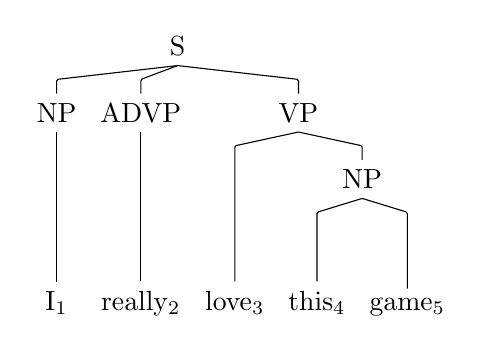
\begin{tikzpicture} [
				level distance=24pt,
				every tree node/.style={align=center,anchor=base},
				frontier/.style={distance from root=92pt},
				edge from parent/.style={draw,edge from parent path={(\tikzparentnode.south) {[rounded corners=0.5pt]-- ($(\tikzchildnode |- \tikzparentnode.south) + (0, -5pt)$) -- (\tikzchildnode)}}}
			]
			\Tree
			[.S
				[.NP I$_1$ ]
				[.ADVP really$_2$ ]
				[.VP love$_3$ [.NP this$_4$ game$_5$ ] ]
			];
		\end{tikzpicture}
		\caption{原始句法树}
		\label{fig:con-original-tree}
	\end{subfigure}
	\hfill
	\begin{subfigure}[b]{0.45\textwidth}
		\centering
		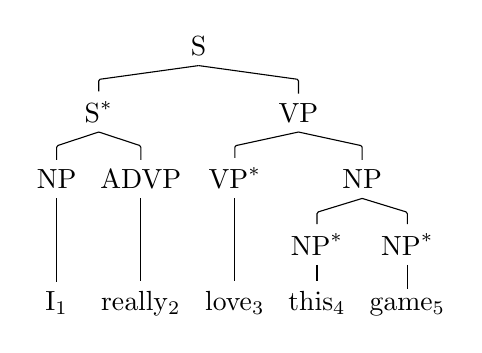
\begin{tikzpicture} [
				level distance=24pt,
				every tree node/.style={align=center,anchor=base},
				frontier/.style={distance from root=92pt},
				edge from parent/.style={draw,edge from parent path={(\tikzparentnode.south) {[rounded corners=0.5pt]-- ($(\tikzchildnode |- \tikzparentnode.south) + (0, -5pt)$) -- (\tikzchildnode)}}}
			]
			\Tree
			[.S
				[.$\textrm{S}^\ast$ [.NP I$_1$ ] [.ADVP really$_2$ ] ]
				[.VP
					[.$\textrm{VP}^\ast$ love$_3$ ]
					[.NP [.$\textrm{NP}^\ast$ this$_4$ ] [.$\textrm{NP}^\ast$ game$_5$ ] ]
				]
			];
		\end{tikzpicture}
		\caption{遵循乔姆斯基范式的左二叉化句法树}
		\label{fig:con-binaried-tree}
	\end{subfigure}
	\caption{
		成分句法树的例子.
		其中词性在这里被忽略
	}
	\label{fig:con-tree-full-figure}
\end{figure}

成分句法则旨在构建一个层次化的树结构.
如图\ref{fig:con-tree-full-figure},其中每个叶子结点是输入句子的每个词,而非终端结点作为区块(Constituents),如$\texttt{VP}_{3,5}$.
正式地,给定一个由$n$个词组成的句子$\boldsymbol{x}=w_1,\dots,w_{n}$,如图~\ref{fig:con-tree-original}所示,一棵成分句法树可以表示为$\boldsymbol{t}=\{((i, j),l)\mid 1\le i \le n,i \le j \le n,l \in \mathcal{L}\}$,其中$((i,j),l) \in \boldsymbol{t}$是一个包含$w_{i}...w_{j}$的区块,对应的句法标签为$l \in \mathcal{L}$.
本文中,为了方便模型处理,我们还将原始的树转换为了二叉树形式,如图~\ref{fig:con-binaried-tree}所示.
成分句法分析相比于依存句法而言,研究历史更加悠久,尽管目前没有依存句法技术那么流行,但是以其分析技术为基础衍生出了一系列在其他任务上的解析方法,例如UCCA语义分析\citep{jiang-etal-2019-hlt}、嵌套命名实体识别\citep{fu-etal-2021-nested}等等

不同于传统句法分析方法十分依赖于离散特征的人工设计,由于深度神经网络的强大上下文编码能力,句法分析器的方法愈来愈有简单化的趋势.
其中依存句法分析器Biaffine Parser\citep{dozat-etal-2017-biaffine}正是符合这样的潮流:利用诸如双向LSTM或Transformer\citep{vaswani-2017-attention}等强大编码器得到上下文表示,然后采取一个简单的头选择训练损失函数训练每个词找到正确的头.
类似的,\citet{gaddy-etal-2018-whats}采用的成分句法分析器采用了一个二分类训练目标,判断每个位置是否能够组成一个区块.
由于其准确率高,速度快的特点,基于局部训练目标的分析器是目前最为流行的句法分析器.

然而,已有的句法分析器Biaffine Parser也存在一些固有的缺陷.
由于训练时没有显式的树结构约束,在解码时分析器仍然需要通过解码算法(例如Eisner算法、MST算法或CKY算法)来得到一棵合法的树,这就造成了训练和预测的不匹配.
由于分析器训练目标较强的独立性假设,尽管能够得到合法的树输出,但是我们没法得到相应的树概率,而在数据建模的时代,概率分布估计一直是一个核心问题\citep{le-zuidema-2014-inside}.

因此,在本文章节~\ref{cha:dep-crf}和章节~\ref{cha:con-crf},分别在依存句法分析任务和成分句法分析任务上,我们考虑将以前流行的结构化学习目标引入到现有的神经网络模型中,我们尝试引入树形条件随机场(TreeCRF)在训练时最大化树的概率.
考虑到在前人的工作中,引入高阶特征一直对于句法分析性能的提升\citet{mcdonald-pereira-2006-online,chen-manning-2014-fast}很关键,因此我们还尝试在两种句法分析范式中尝试了采用兄弟等二阶子树特征.
在我们之前,已经有研究者尝试在神经网络模型中增加高阶建模和结构化学习\citep{zhang-etal-2019-empirical,falenska-kuhn-2019-non}.
然而,引入更多的高阶特征后结构化学习算法受限于高复杂度问题,限制了该类算法的广泛应用.
我们主要从两个方面尝试缓解这类算法的高复杂度问题.
第一,得益于GPU的并行计算能力,我们为结构化学习的精确推断算法,诸如(二阶)Inside算法等设计了精巧的批次化方法,使得推断过程能够在GPU上能够利用到并行计算大大加速.
第二,有益于集成了自动求导机制的深度学习库的出现,我们无需和前人一样需要在CPU上进行完整的Inside-Outside过程得到梯度,而是由结合自动求导的反向传播机制自动完成.

在机器学习社区中,研究者在针对推断算法高复杂度或者不可精确推断的问题时,通常的做法是尝试采用近似算法来进行近似推断.
因此在章节~\ref{cha:vi}中,我们还尝试了利用机器学习中的一个近似推断算法,平均场变分推断(Mean Field Variational Inference, \textsc{Mfvi}),近似得到后验概率,我们在依存句法和成分句法分析两种范式中分别设计了两种不同的因子图以及变分推断迭代算法,显著提升了句法分析方法的解析速度.

\section{数据集和评价指标}

\begin{table}[tb!]
    \centering
    \caption{依存句法分析数据集的数据统计,包含句子数和标签数.}
    \begin{tabular}{lrrr|c}
        \toprule
                & \#Train & \#Dev & \#Test & \#labels \\[1pt]
        \midrule
        % \\[-8pt]
        PTB     & 39,832  & 1,700 & 2,416  & 45       \\
        CoNLL09 & 22,071  & 1,762 & 2,556  & 41       \\
        NLPCC19 & 29,991  & 4,098 & 8,295  & 22       \\
        \bottomrule
    \end{tabular}
    \label{table:dep-statistics}
\end{table}

\noindent\textbf{数据.}
对于依存句法分析,我们在13个语言的27个数据集上进行了实验和分析,包含两个广泛使用的数据集:英语的斯坦福依存规范\citep{chen-manning-2014-fast}的宾州树库(Penn Treebank, PTB)和中文的CoNLL09数据\citep{hajic-etal-2009-conll}.
我们还采用了公开于NLPCC19跨领域句法分析任务的中文数据集\citep{peng-etal-2019-overview},其中一共包含了四个源领域和三个目标领域.
方便起见,我们直接合并了四个领域的Train/Dev/Test数据到更大的数据集.
这些数据的一个特征是大部分句子都是利用基于主动学习的局部标注得到的.
表~\ref{table:dep-statistics}列出了相关数据的统计信息.
最后,遵循\citep{ji-etal-2019-graph}和\citep{zhang-etal-2019-empirical},我们在Universal Dependencies (UD) v2.2和v2.3上进行了实验.
我们采用了\citet{zeman-etal-2018-conll}使用的300维多语言预训练词向量,并采用CharLSTM表示作为输入.
对于UD2.2,为了和\citet{ji-etal-2019-graph}公平比较,我们和CoNLL18任务一样\citep{zeman-etal-2018-conll},使用了毛文本,并且直接使用了他们的句子分割和符号化的结果.
对于UD2.3,为了与\citet{zhang-etal-2019-empirical}比较,我们报告的结果使用了正确词性.

对于成分句法分析,我们主要在三个中文和英文的数据集上进行实验.
前两个数据集,即PTB和CTB5.1,是句法分析社区中比较常用的两个数据集.
我们遵循了传统的Train/Dev/Test数据分割.
考虑到CTB5.1的Dev/Test都只有大约350句,为了得到更加稳定一致的结果,我们还在更大的CTB7数据上进行了实验,相关的数据分割设置参考了官方手册建议.
表~\ref{table:con-statistics}列出了相关数据的统计信息.
可以看到CNF转换引入了很多新的区块标签,其中大部分(大约75\%)都源于连续单链的折叠过程.

\begin{table}[tb!]
    \centering
    \caption{数据统计,包含句子数和标签树.
        对于``\#labels'',我们列出了原始树和CNF树对应的标签数.}
    \begin{tabular}{lrrr|ccc}
        \toprule
               & \multirow{2}{*}{\#Train} & \multirow{2}{*}{\#Dev} & \multirow{2}{*}{\#Test} & \multicolumn{2}{c}{\#labels}       \\
               &                          &                        &                         & original                     & CNF \\[1pt]
        \midrule
        % \\[-8pt]
        PTB    & 39,832                   & 1,700                  & 2,416                   & 26                           & 138 \\
        CTB5.1 & 18,104                   & 352                    & 348                     & 26                           & 162 \\
        CTB7   & 46,572                   & 2,079                  & 2,796                   & 28                           & 265 \\
        \bottomrule
    \end{tabular}
    \label{table:con-statistics}
\end{table}

\noindent\textbf{评价指标.}
对于依存句法分析,我们使用无标签/有标签附着分值(Unlabeled/Labeled Attachment Score, UAS/LAS)作为主要的评价指标.
评价时,PTB中的词性会被忽略掉.
对于局部标注的NLPCC19数据,我们采用了官方的评价脚本,直接忽略了没有正确头标注的词.
我们采用了Dan Bikel的随机解析评价比较器来进行显著性检验.

对于成分句法分析,正如前面提到的,在解析之后,我们将最佳的CNF树转化为了\textit{n}-ary树再进行评价.
这里有必要提及一些有用的细节.
由于解码算法没有相应的约束,预测的最佳CNF树可能包含很多不合法的产生式.
以图~\ref{fig:con-binaried-tree}为例,模型可能输出$\texttt{VP}_{3,5} \rightarrow \texttt{PP}^{\ast}_{3,3} ~ \texttt{NP}_{4,5}$,其中 $\texttt{VP}$和$\texttt{PP}^{\ast}$是不兼容的.
在\textit{n}-ary后处理过程中,我们直接忽略了``$\mathtt{\ast}$''符号之前具体的字符串$\texttt{PP}$.
有鉴于此,如果解码的时候增加一定的约束,结果有可能进一步提高,这里我们留待作为后续的工作.
我们使用了标准的区块级别的准确率、召回率和$\mathrm{F}_1$值($\mathrm{P}$/$\mathrm{R}$/$\mathrm{F}_1$)作为评价指标,并使用\texttt{EVALB}工具\footnote{\url{https://nlp.cs.nyu.edu/evalb}}来评价.
特别地,一个例如$\texttt{VP}_{3,5}$的预测区块如果出现在了正确树中,那就被认为是正确的.\footnote{
    由于一些研究者可能会实现他们自己的评价脚本,为了比较的公平,需要澄清一些细节:
    1)一些诸如\texttt{\{-NONE-\}}的空区块在预处理的时候被移除了.
    2)评价的时候作为根结点的区块(英语里是\texttt{\{TOP,S1\}},中文里是空字符串) 被忽略了.
    3)包含一些例如\texttt{\{:,``,'',.,?,!\}}这些标点的区块也被忽略了. 请注意中文标点会作为正常的字符被评价.
    4)一些在同一集合中的标签,例如\texttt{\{ADVP,PRT\}},被认为是等价的.}

\section{相关工作}
\label{sec:relworks}

\subsection{依存句法分析}

批次化技术已经在线性链条件随机场(linear-chain CRF)中广泛应用,但是在树形结构中这个要复杂得多.
\citet{eisner-2016-inside}在成分句法分析上提出了一个关于Outside算法和反向传播机制等价性的理论证明,并同样讨论了其他类似于依存文法的范式.
我们在章节~\ref{cha:dep-crf}的工作中借鉴了他们的理论性工作.
作为一个经验型分析,我们相信我们的尝试能够让树形条件随机场在现实系统中应用起来.

和\citet{gaddy-etal-2018-whats}在成分句法上的工作类似,\citet{falenska-kuhn-2019-non}提出了一个在依存句法上的很好的分析性工作.
通过将\citet{kiperwasser-goldberg-2016-simple}的一阶基于图的方法扩展到二阶,他们尝试探究有多少结构化上下文被双向LSTM编码器捕捉.
他们拼接3层LSTM的在$i,k,j$位置的输出向量来给邻接兄弟子树打分,并采用了Max Margin训练损失和二阶Eisner解码算法\citep{mcdonald-pereira-2006-online}.
基于他们相对负面的结果和分析,他们认为高阶建模是多余的,因为双向LSTM已经可以有效的隐式捕捉足够的结构化上下文.
他们同样在RNNs和句法的关系上进行了详细的调研.
在我们的工作中,我们使用了一个更强的基线模型,并且发现了相比于他们的工作更显著的UAS/LAS提升.
特别地,我们提出了深入的分析,显示显式建模高阶信息可以帮助句法模型,因此与双向LSTM编码器是互补的.


\citet{ji-etal-2019-graph}引入了高阶结构信息,并用在Biaffine Parser\citep{dozat-etal-2017-biaffine}上用图神经网络来隐式建模.
他们在MLP层和Biaffine层之间增加了三层的图注意力网络(graph attention network,GAT)\citep{velickovic-etal-2018-graph}作为组块.
第一层GAT使用MLP层的输出$\mathbf{r}_i^{h}$和$\mathbf{r}_i^{m}$作为输入,通过集聚邻居节点产生新的表示$\mathbf{r}_i^{h1}$和$\mathbf{r}_i^{m1}$.
类似的,第二层GAT在$\mathbf{r}_i^{h1}$和$\mathbf{r}_i^{m1}$上操作,产生$\mathbf{r}_i^{h2}$和$\mathbf{r}_i^{m2}$.
通过这种方式,一个节点渐渐的收集到多跳的高阶信息作为单条弧打分的全局证据.
训练时他们遵循了原始的头选择训练损失.
与此相对的,我们的工作采用的全局的TreeCRF损失并显式地将高阶分值引入到了Biaffine Parser.

\citet{zhang-etal-2019-empirical}探索了在一阶Biaffine Parser上结构化学习的作用.
他们在多语言数据上比较了局部头选择损失、全局Max Margin损失和TreeCRF损失的性能.
他们表明全局的TreeCRF损失总体上要稍微好于Max Margin损失,并且对大多数语言而言,结构化学习带来了虽然不多但是显著的LAS提升.
他们同样表明结构化学习,特别是TreeCRF,极大的提升了句子级匹配的准确率,这与我们的观察相仿.
此外,他们通过Cython programming显式在CPU上计算了Inside算法和Outside算法.
与此对应的,这里我们在Biaffine Parser上提出一个高效的二阶TreeCRF扩展,并且进行了更加深入的分析,证明了结构化学习和高阶建模的效果.

\subsection{成分句法分析}

由于效率低下,以前很少有关于条件随机场的成分句法分析的工作.
\citet{finkel-etal-2008-efficient}提出了第一个基于非神经网络的引入丰富特征的条件随机场成分句法分析器.
\citet{durrett-klein-2015-neural}拓展了\citet{finkel-etal-2008-efficient}的工作,使用一个带非线性激活的前馈神经网络来打分产生式.
这两个工作都在CPU上显式进行了Inside-Outside计算,并且有严重的效率问题.

我们的成分句法分析器基于高性能的基于双向LSTM编码器\citep{stern-etal-2017-minimal}的现代神经网络分析器,在基于图的模型上利用了minus feature\citep{cross-huang-2016-span}进行区块的打分.
最近有很多工作都参考了\citet{stern-etal-2017-minimal}.
\citet{gaddy-etal-2018-whats}尝试分析什么样的,以及有多少上下文被双向LSTM隐式编码.
\citet{kitaev-klein-2018-constituency}将2层双向LSTM替换为自注意力层,并通过分离上下文和位置注意力,发现了可观的提升.
与此对应的,我们的工作表明通过合理的设置双向LSTM,例如Dropout策略,\citet{stern-etal-2017-minimal}的分析器可以超过\citet{kitaev-klein-2018-constituency}的结果.
请注意\citet{kitaev-klein-2018-constituency}的工作中使用了很大的词向量.

对于序列标注任务而言,批次化很直接,并且已经被很好的解决,比如NCRF++的实现\footnote{\url{https://github.com/jiesutd/NCRFpp}}.
但是,还很少有工作关注树形结构.
在依存句法的工作里,我们首次提出批次化树形结构的Inside和Viterbi(Eisner)计算,以便于在依存句法分析中利用GPU加速\citep{zhang-etal-2020-efficient}.
现在,我们在成分句法分析中做了类似的扩展,采用了不同的Inside和Viterbi(CKY)算法.

Torch-Struct\footnote{\url{https://github.com/harvardnlp/pytorch-struct}}\citep{rush-2020-torch}是我们的方法之外一个同期独立完成的工作,同样为成分句法分析实现了批次化的CKY算法.
然而,Torch-Struct旨在实现通用目的的结构化预测算法的基本实现.
与此相反,我们着力于复杂的解析器模型,并力求达到成分句法分析在准确率和效率上的最佳性能.

与此同时,近期有许多工作没有显式考虑结构化约束或者CKY解码,极大简化了成分句法分析任务.
\citet{gomez-rodriguez-vilares-2018-constituent}通过对每个词设计复杂的标签编码树信息,尝试采用序列标注方法解决成分句法分析任务.
\citet{vilares-etal-2019-better}通过一系列的增强技术,例如多任务学习和策略提督,进一步增强的序列标注方法.
\citet{shen-etal-2018-straight}提出对于正确树中的每个邻居词对预测一个数值距离,并应用自底向上的贪婪解码找到一棵最优的树.
然而,所有上面的工作仍然在解析性能上极大的落后于主流的方法.

\subsection{高阶句法分析方法}

\subsection{近似推断方法}
尽管引入高阶特征,能够帮助模型准确率的提升\citep{mcdonald-pereira-2006-online,carreras-2007-experiments,koo-collins-2010-efficient,ma-zhao-2012-fourth},
然而这种高阶特征通常导致难以设计一个精确推断的算法来得到目标结构的概率,进而最大化概率来优化模型,甚至对于非投影依存句法分析而言,高阶模型推断算法是NP-hard问题\citep{mcdonald-pereira-2006-online}.
因此我们不得不考虑近似方法.
由于结构化学习问题中不可精确推断问题的广泛存在,因此一直以来近似推断算法在NLP社区都有很多都应用.

\citet{martins-etal-2009-concise}将依存句法分析问题近似为整数线性规划(Integer Linear Programming, ILP)问题.
与传统算法相比,他们利用了大量的局部和全局丰富特征,例如兄弟、祖父特征和价键特征,作为线性约束,用ILP来求解,保证输出是一棵合法的依存树.
\citet{koo-etal-2010-dual}将非投影依存句法分析形式化为对偶分解(Dual Decomposition, DD)问题,即将一个难以求解的问题分解为若干个可求解的子问题,例如可以将输出树的问题分解到单条弧、连续兄弟、双头等子结构上\citep{martins-etal-2011-dual}.

另一个和我们的在本文采用的平均场变分推断高度相关的方法是循环置信传播(Loopy Belief Propagation, LBP).
循环置信传播定义了一个包含多种局部和全局特征的由变量和因子构成的因子图,接着算法迭代式地让因子(变量)收集邻居变量(因子)的信息,最终收敛后得到后验概率.
\cite{smith-eisner-2008-dependency,gormley-etal-2015-approximation}在依存句法分析上引入了循环置信传播.
除了上面提到的兄弟(\textsc{Sib})、祖父(\textsc{Grand})因子,他们还引入了丰富的全局因子,例如\textsc{Exactly1}约束每个词有且仅有一个头,\textsc{Tree}要求所有词必须组成一棵树等等.
\citet{naradowsky-etal-2012-grammarless}将循环置信传播引入到了成分句法分析,也采用了类似的高阶因子(如\textsc{Tree})在成分句法上的变体.
与精确算法相比,循环置信传播可以用可接受的复杂度引入大量全局因子,并为模型带来了可观的性能收益.

还有一些工作同时使用了上述的近似算法.
\citet{auli-lopez-2011-comparison}在组合范畴文法中同时采用了循环置信传播\citep{smith-eisner-2008-dependency}以及对偶分解\citep{koo-etal-2010-dual},取得了最佳性能,并对两种方法做了经验性比较.
\citet{martins-etal-2010-turbo}提出了在非投影依存句法分析中同时利用了循环置信传播\citep{smith-eisner-2008-dependency}以及整数线性规划\citep{martins-etal-2009-concise}方法,表明两种方法采用了一致的因子图,并在局部近似的目标函数的理念上是相一致的.

近期在神经网络模型上,涌现出了大量的关于近似推断在结构化预测任务等上的应用\citep{li-etal-2020-high,wang-etal-2020-ain}.
\citet{wang-etal-2019-second}首次在基于图的语义依存分析上提出了二阶模型,并采用LBP和MFVI作为近似算法,观察到了两种推断算法相似的性能提升.
\citet{wang-tu-2020-second}首次在依存句法分析中引入了MFVI,他们采用了兄弟、组合和共同父亲这三种二阶特征.
我们的依存模型中采用的基于头选择的MFVI参考了\citet{wang-tu-2020-second},为了和精确推断算法公平比较,本文中我们只保留了兄弟特征.
上述工作引入了近似推断算法之后都达到了和精确推断可比较的结果,同时速度上大大提升,这和我们的发现是一致的.

\section{章节和内容安排}

本文共分为五个章节,各章节具体安排如下:

第一章 绪论. 本章介绍本文中每个工作的任务背景和意义,并阐述一下与工作相关的有关文献的进展和内容,以及与我们方法的对比.

第二章 基于树形条件随机场的高阶依存句法分析.
本章在当前最佳的依存句法分析器的基础上,提出了一个二阶树形条件随机场的拓展,进一步提升了句法分析的性能.
为了解决效率问题,我们还提出了批次化技术在GPU上对训练和解码算法进行加速.

第三章 基于树形条件随机场的快速精准成分句法分析.
本章将树形条件随机场的应用到了神经成分句法分析器当中.
我们应用了批次化技术解决了树形条件随机场效率低下的问题.
我们提出了一个简单的两阶段解析方法,来进一步提升分析器的效率.
我们还为解析器引入了新的打分架构,以及有效的Dropout策略,使得解析器达到了新的最佳水平,并且解析速度很快.

第四章 基于变分推断的高效句法分析方法.
本章在前面章节提出的高阶句法分析器的基础上,提出利用平均场变分推断方法来近似推断后验概率.
在引入高阶算法的同时,变分推断避免了精确推断算法的高复杂度问题,并达到了和精确推断方法接近或相当的结果.

第五章 总结与展望. 本章总结本文的主要内容,并展望后续可能的研究方向.
\chapter{基于树形条件随机场的高效依存句法分析}
本章首先分析了第\ref{sec:super_tc}章提出的树库转化方法和树库融合方法的不足之处,然后针对这两方面进行改进.
一方面,为了深度、高效地编码源端句法树,我们改进基于SP-TreeLSTM方法,并提出基于Full-TreeLSTM的树库转化方法,提升了转化模型的速度和性能;
另一方面,为了缓解转化后树库中存在的噪音问题,我们尝试了两种简单有效的树库融合方法,即语料加权方法以及合并后微调方法,更加合理地使用了转化后树库,进一步提升了目标端句法模型的性能.
%最后,相较于之前树库转化方法的级联模型,我们提出一种更为简洁的耦合性更强的基于多任务学习的依存句法-树库转化的联合模型.
%除了利用上一章的转化数据$CODT^{\texttt{PCTB7}}$
最后,为了得到更可靠的实验结果和结论,我们额外构建了一份双树对齐数据$CODT^{\texttt{PCTB7}}$,本章所有的方法均在两份转化语料上进行实验.

\section{引言}
\input{figures/dep-example.tex}
依存句法分析任务是NLP领域的一个基础性任务,由于其简洁性,以及可以方便的在多语言上获得句法和语义信息的特性,目前在这一任务上已经有了大量的研究. 如图\ref{fig:dep-tree-example}所示,给定一个句子$\boldsymbol{x}=w_0w_1\cdots w_n$,一棵依存树被定义为$\boldsymbol{y}=\{(i,j,l),0\le i \le n,1 \le j \le n,l \in \mathcal{L}\}$,其中$(i,j,l)$是一条从头(head)$w_i$到修饰词(modifier)$w_j$的弧,弧的标签为$l \in \mathcal{L}$. 目前在依存句法分析任务上有两个主流方法,分别是基于转移(transition-based)的方法,和基于图(graph-based)的方法,这里我们的方法主要关注于基于图的解析方式.

在深度学习时代之前,基于图的解析依赖于很多手工特征的设计,比如词性、前缀、后缀等等.
与神经网络方法相比,以前的方法有两个显著的不同.
首先,对于非神经网络方法而言,结构化学习(结构化学习)是不可或缺的,即训练时需要显式地建模树结构的约束.
通常此类方法采用的是max-margin训练算法,首先用当前模型训练一棵分值最高的树,然后更新模型参数,以保证正确的树的分值要高于预测树.

第二个显著的区别在于高阶特征的使用. 高阶特征为模型带来了显著的提升.
基础的一阶模型将句法树的分值分解为若干条独立的弧的分值\cite{mcdonald-etal-2005-online}. 后续的工作进一步引入了二阶依存弧对对分值,比如邻接兄弟\cite{mcdonald-pereira-2006-online}和祖父-父亲-孩子这样的弧对\cite{carreras-2007-experiments,koo-collins-2010-efficient},这些高阶扩展都带来了模型性能的显著提升\footnote{三阶和四阶模型的提升不大,这可能是由于特征稀疏的问题导致的\cite{koo-collins-2010-efficient,ma-zhao-2012-fourth}.}. 但是这些高阶模型需要引入更复杂的解码算法,导致了模型更加低效.


相比之下,基于图的神经网络依存句法分析器的发展呈现出相反的趋势.
\cite{pei-etal-2015-effective}提出利用前馈神经网络来自动学习\cite{chen-manning-2014-fast}的若干特征组合,并计算子树得分.
他们的工作表明引入二阶邻接兄弟子树的分值显著提高了性能。
随后,\cite{wang-chang-2016-graph}和\cite{kiperwasser-goldberg-2016-simple}都建议使用BiLSTM作为编码器和,以及在一阶模型中利用minus-feature来对单条弧打分.
这三个代表性方法都采用了全局的max-margin方法.
\cite{Timothy-d17-biaffine}提出了一种强大而高效的Biaffine Parser,并在各种数据集和语言上获得了最先进的精度.
Biaffine Parser也是一阶的,通过对每个词进行局部头选择(head selection)的方式\cite{zhang-etal-2017-dependency-parsing},采用了更简单、更有效的非结构化训练方法.

基于这些对比,我们尝试在基于图的解析器的基础上,将前深度学习时代的一些方法与神经网络模型做一下连接.
这里要解决的\textbf{第一个问题}是:
\emph{以前的一些技术,比如结构化学习和高阶建模,能够进一步提升当前最佳的解析器Biaffine Parser的性能吗\footnote{
        尽管最近的一些工作汇报了相比Biaffin Parser更高的性能,但是都引入了一些外部资源,比如大规模语言模型的上下文词表示. 在相同网络和相同实验设置的场景下,这些工作的结果都是相近的.
    },如果可以,他们在哪些方面是有用的?}

对于结构化学习而言,相比max-margin方法,我们采用更复杂且更不常用的TreeCRF.
主要原因有两方面.
首先,概率分布估计一直是当前数据驱动的NLP方法的一个核心的问题\cite{le-zuidema-2014-inside}.
如果将解析器的输出应用到更高层的任务,一棵句法树的概率$p(\boldsymbol{y}\mid\boldsymbol{x})$比没有上下边界的分值$s (\boldsymbol{x},\boldsymbol{y})$一般而言要更加有用.
其次,边缘概率是一种理论上比较可靠的方法来评估模型输出子树的置信度,可以用于最小贝叶斯风险(MBR)解码\cite{smith-smith-2007-probabilistic},并且已经被证明了对于词级别基于局部标注句法树的主动学习(active learning)\cite{li-etal-2016-active}很有用.

尽管很有用,但是TreeCRF不如max-margin那么留下,其中一个原因是由于inside-outside算法的高复杂度,尤其是outside算法.
据我们所知,所有现存的模型都是在CPU上运算inside-outside算法.
而由于CPU/GPU巨大的效率差异,这一低效的问题在深度学习时代变得更加严重.
这就引发了\textbf{第二个问题}:
\emph{我们是否能够批次化inside-outside算法,并且直接在GPU上进行计算?}
如果这样的话,我们就能够利用诸如PyTorch这样的高效深度学习张量库来进行计算,并且将高效的TreeCRF应用到更多的场景\cite{cai-etal-2017-crf,le-zuidema-2014-inside}.

总体而言,针对上面的两个问题,我们做了下面的几个贡献:
\begin{itemize}%[leftmargin=10pt,topsep=3pt,itemsep=1pt,partopsep=1pt]
    \item 我们第一次提出了将二阶TreeCRF应用到神经依存句法分析中.
          我们还提出了一个高效的Triaffine结构来对于二阶子树打分.
    \item 我们提出通过GPU上大规模的并行张量计算来批次化inside算法,来进行更高效的TreeCRF损失函数的计算.
          我们表明复杂的outside算法对于梯度和边缘概率的计算而言已不再必须,相应的可以用高效的反向传播代替.
    \item 我们在13个语言的27个树库上进行了实验.
          结果和分析都表明,深度学习时代的,结构化学习和高阶建模在许多方面对当前最好的Biaffine Parser仍然是有用的.
\end{itemize}

\section{基线模型}
\label{section:basic_model}


We re-implement the state-of-the-art biaffine parser \cite{Timothy-d17-biaffine} with
% We follow their work in all important details such as dropouts and initialization.
two modifications, i.e., using CharLSTM word representation vectors instead of POS tag embeddings, and
the first-order Eisner algorithm \cite{eisner-2000-iwptbook}
for projective decoding instead of the non-projective MST algorithm.

\paragraph{Scoring architecture.}
%(Figure~\ref{fig:biaffine-parser-architecture})}
Figure~\ref{fig:framework} shows the scoring architecture, consisting of four components.

% The basic architecture of our model is mainly based on that of .
% In this section, we describe the components of the basic parsing model in a top-down fashion.

% We then introduce the scoring functions which are capable of capturing the relations of head-modifier pairs or even higher order.

%We first have a review of the word encoding part.

% 先别删这句话:最后的数学符号要过一遍,统一一下,严谨!粗体、斜体、大小写等

\subparagraph{Input vectors.}
The $i$th input vector % for the $i$th word
is composed of two parts:
the word embedding and the CharLSTM word representation vector of $w_i$.
\begin{equation}
    \label{equation:input}
    \mathbf{e}_i=\mathrm{emb}({w_i}) \oplus \mathrm{CharLSTM}(w_i)
\end{equation}
where $\mathrm{CharLSTM}(w_i)$ is obtained by feeding $w_i$ into a BiLSTM and
then concatenating the two last hidden vectors \cite{lample-etal-2016-neural}.
We find that replacing POS tag embeddings with  $\mathrm{CharLSTM}(w_i)$ leads to consistent improvement,
and also simplifies the multilingual experiments by avoiding POS tag generation (especially n-fold jackknifing on training data).
%Compared with POS tag embeddings, we find that
%where $\mathbf{e}_i$ is the concatenation of the word embedding $\mathbf{e}_i^{w}$ and character-level embedding $\mathbf{e}_i^{c}$.
%$\mathbf{e}_i^{c}$ is acquired by concatenating the last hidden states produced by the BiLSTM performing on the word characters \cite{lample-etal-2016-neural}.

%Since subsequent researchers have show the effectiveness of character-level embeddings \cite{dozat-etal-2017-stanfords,kitaev-klein-2018-constituency},
%we make a few modifications for the input that replacing the Part-of-Speech (POS) Tag embeddings with \textsc{CharLSTM} word representations.
%Given a sentence $\boldsymbol{x}=w_0,w_1, \ldots, w_n$, where $w_0$ denotes the root node, each word $w_i$ is mapped into a dense vector $\mathbf{e}_i$
% \footnote{
% We adopt the convention of \citet{Timothy-d17-biaffine} that uses lowercase italics for scalars, lowercase bold for vectors, uppercase italics for matrices, and uppercase bold for tensors.
% },

\subparagraph{BiLSTM encoder.} To encode the sentential contexts,
the parser applies three BiLSTM layers %are applied
over %the input vector sequence
$\mathbf{e}_0 \dots \mathbf{e}_n$. The output vector of the top-layer BiLSTM for the $i$th word
is denoted as $\mathbf{h}_i$.
%The $i$th
%Then we use the corresponding hidden output for parsing, denoted as $\mathbf{r}_i$.
%We use  to denote .

\subparagraph{MLP feature extraction.} Two shared MLPs are applied to $\mathbf{h}_i$, obtaining
two lower-dimensional vectors that detain only syntax-related features:
\begin{equation}
    \label{mlp-arc}
    %\mathbf{r}_i^{h}; \mathbf{r}_i^{m} =\mathrm{MLP}_{h/m} (\mathbf{h}_i);\mathrm{MLP}_{m} (\mathbf{h}_i)
    \mathbf{r}_i^{h}; \mathbf{r}_i^{m} =\mathrm{MLP}^{h/m} \left( \mathbf{h}_i \right)
\end{equation}
where $\mathbf{r}_i^{h}$ and $\mathbf{r}_i^{m}$ are the representation vector of $w_i$ as a head word and a modifier word respectively.


\subparagraph{Biaffine scorer.}
%Biaffine计算效率很高。
%Recent works regard graph-based dependency parsing as a head selection task \cite{zhang-etal-2017-dependency-parsing,Timothy-d17-biaffine}.
%For each word pair ($w_i$, $w_j$), they assign it a score to measure how possible the word $w_j$ modifies $w_i$,
%and select the one with the highest score one as the resulting head-dependent pair.
%As a representative job,
\citet{Timothy-d17-biaffine} for the first time propose to compute the score of a dependency $i \rightarrow j$ via biaffine attention:
%  design a very subtle biaffine operation.
\begin{equation} \label{equation:biaffine}
    %score(i, j) =  \big[{{\mathbf r_i^{D}} \oplus {\mathbf{1}}} \big]^\textup T   W^b  \mathbf r_j^{H}
    s(i,j) =  \left[
        \begin{array}{c}
            \mathbf{r}_{j}^{m} \\
            1
        \end{array}
        \right]^\mathrm{T}
    \mathbf{W}^\textit{biaffine}  \mathbf{r}_{i}^{h}
\end{equation}
where $\mathbf{W}^\textit{biaffine} \in \mathbb{R}^{d \times d}$.
The computation is %straightforward to batchify on GPUs and thus
extremely efficient on GPUs.
%Specifically, they first apply MLP layers on $\mathbf{r}_i$ to obtain the representations of each word as a head ($\mathbf{h}_i^{arc}$) and as a dependent ($\mathbf{d}_i^{arc}$):
%As discussed in \citet{Timothy-d17-biaffine}, the MLP layers on the one hand reduces the dimensionality of $\mathbf{r}_i$,
%and more importantly on the other hand strips away syntax-unrelated information and thus avoids the risk of over-fitting.


\begin{figure}[tb]
    \centering
    \includegraphics{figures/framework.pdf}
    \caption{Scoring architecture with second-order extension.
        %可否把7个MLP都画出来,然后label部分的biaffine画成层叠的,表示有多个。
        %不,就画5个,我会在正文中专门讲label的处理;
        %然后biaffine和triaffine输出加上$\mathrm{s}(i,j,l)$, $\mathrm{s}(i,j)$, $\mathrm{s}(i,k,j)$等
    }
    \label{fig:framework}
    % \vspace{-5pt}
\end{figure}

\paragraph{Local token-wise training loss.}
The biaffine parser adopts a simple non-structural training loss,
trying to independently maximize the local probability of the correct head word for each word.
%For a gold-standard dependency $i \rightarrow j$
For a gold-standard head-modifier pair ($w_i$, $w_j$)
in a training instance,
%For $w_j$ and its gold-standard head $w_i$,
the cross-entropy loss is
\begin{equation} \label{equation:biaffine-loss}
    \mathit{L}(i,j) = -\log{\frac{e^{s(i,j)}}{\sum_{0 \le k \le n} e^{s(k,j)}}}
    % & -\log{
    % \frac{e^{\texttt{score}(i \xleftarrow{l} j)}}
    % {\sum_{l' \in \mathcal{L}} e^{\texttt{score}(i \xleftarrow{l'} j)}}
    % }
\end{equation}
%where $\mathcal{L}$ is the label set.
In other words, the model is trained based on simple head selection,
without considering the tree structure at all, and
losses of all words in a mini-batch are accumulated.

\paragraph{Decoding.} Having scores of all dependencies,
we adopt the first-order Eisner algorithm with time complexity of $O(n^3)$
to find the optimal tree.
\begin{equation}
    \label{equation:map-decoding}
    {\boldsymbol{y}}^* = \arg\max_{\boldsymbol{y}} \left[ s(\boldsymbol{x},\boldsymbol{y}) \equiv
        %& s(\boldsymbol{x},\boldsymbol{y}) =
        \sum_{i \rightarrow j \in \boldsymbol{y}}{s(i,j)} \right]
\end{equation}
% 这段话考虑移到其他地方。
% Since this work focuses on projective dependency parsing,
% we adopt the pseudo-projective approach \cite{nivre-nilsson-2005-pseudo} for handling non-projective datasets. % with non-projective trees.
% The idea is to transform non-projective trees in projective ones using more complex labels for post-processing recovery.

\paragraph{Handling dependency labels.}
The biaffine parser treats skeletal tree searching and labeling as two independent (training phase) and cascaded (parsing phase) tasks.
This work follows the same strategy for simplicity. Please refer to \citet{Timothy-d17-biaffine} for details.

% Then a biaffine layer is used to compute scores of all dependencies.
% For pair ($i$, $j$), the score function $\mathrm{s}(i, j)$ is defined as
% \begin{equation}
% \mathrm{s}(i, j)=\mathbf{h}_i^{T}W\mathbf{d}_j+\mathbf{u}^T\mathbf{h}_i
% \end{equation}
% where $W \in \mathbb{R}^{d \times d}$ and $\mathbf{u}$ are weight parameters. For simplicity, we omit some superscripts in the formula.

% For dependency labels, extra MLP and Biaffine layers are used to compute the scores $\mathrm{s}(i, j, l)$, where $l$ is the label on the edge ($w_i$, $w_j$)
% We omit the details for brevity.

% During training, for the gold head-dependent pair ($w_i$, $w_j$) , we use the cross-entropy loss to maximize the probability of $w_i$ being the head against all
% words, i.e.,
% $\frac{\exp \mathrm{s}(i, j)}{\sum_{0 \le j^{\prime} \le n} \exp \mathrm{s}(i, j^{\prime})}$.

% \paragraph{Decoding.}
% To ensure well-formedness, we follow two strategies of prior works.
% For treebanks like PTB that contains very few non-projective arcs, we apply the Eisner algorithm to form a valid tree.
% For treebanks that contain a lot of non-projective arcs, we first convert them to pseudo-projective and then apply the Eisner algorithm.
% We have also tried the mst algorithm used in \citet{Timothy-d17-biaffine}. Results show that it is slightly inferior to pseudo-projective ones.
% We leave detailed discussions in Section \ref{section:experiments-analysis}.


% \begin{figure}[tb]
% \subfigure[single dependency] {
%   \begin{minipage}[b]{0.22\textwidth}
%   \centering
%   \includegraphics{figures/scoring-part/a.pdf}
%   \label{fig:scoring-part-a}
%   \end{minipage}
% }
% \subfigure[adjacent sibling] {
%   \begin{minipage}[b]{0.22\textwidth}
%   \centering
%   \includegraphics{figures/scoring-part/b.pdf}
%   \label{fig:scoring-part-b}
%   \end{minipage}
% }
% \caption{The two types of scoring subtrees.}
% \label{fig:scoring-part}

\section{Second-order TreeCRF}
\label{2o-tree-crf}

%\citet{Timothy-d17-biaffine} only take into account the first-order part, i.e., the head-dependent relation in their parsing system.
%Recently, several fruitful investigations have been made on integrating higher-order structured features \cite{mcdonald-pereira-2006-online,carreras-2007-experiments,koo-collins-2010-efficient,ma-zhao-2012-fourth}.
%Considering that their architectures might not be competitive with the current state-of-the-art work, in this paper, we extend the biaffine parser by utilizing high-order parts.

This work substantially extends the biaffine parser in two closely related aspects:
using probabilistic TreeCRF for structural training and explicitly incorporating high-order subtree scores.
%using probabilistic TreeCRF for structural training, and incorporating second-order modeling.
%First, under the second-order modeling,
Specifically, we further incorporate adjacent-sibling subtree scores into the basic first-order model:\footnote{
    This work can be further extended to incorporate
    grand-parent-modifier subtree scores
    %can be realized based on the techniques presented in this work
    %by extending
    based on the viterbi algorithm of $O(n^4)$ time complexity proposed by \citet{koo-collins-2010-efficient}, which
    %, requiring
    we leave for future work.
}
%the score of a tree
\begin{equation}\label{eq:score-definition-2o}
    s(\boldsymbol{x}, \boldsymbol{y}) = \sum_{i\rightarrow j \in \boldsymbol{y}}s(i,j) + \sum_{
        %\begin{array}{c}
        i\rightarrow \{k,j\} \in \boldsymbol{y} %\
        %  i\rightarrow k \in \boldsymbol{y}
        %\end{array}
    } s(i,k,j)
\end{equation}
where $k$ and $j$ are two adjacent modifiers of $i$ and satisfy either $i < k < j$ or $j < k < i$.
%s(\boldsymbol{x}, \boldsymbol{y}) = \sum_{i\rightarrow j \in \boldsymbol{y}}

As a probabilistic model, TreeCRF computes the conditional probability of a tree as
\begin{equation}\label{equation:prob-labeled}
    \begin{split}
        & p(\boldsymbol{y}\mid\boldsymbol{x})  = \frac{e^{s(\boldsymbol{x},\boldsymbol{y})}}{Z(\boldsymbol{x}) \equiv \sum_{\boldsymbol{y'} \in \mathcal{Y}(\boldsymbol{x})} {e^{s(\boldsymbol{x},\boldsymbol{y'})}}}
    \end{split}
\end{equation}
where $\mathcal{Y}(\boldsymbol{x})$ is the set of all legal (projective) trees for $\boldsymbol{x}$, and
$Z(\boldsymbol{x})$ is commonly referred to as the normalization (or partition) term.

During training, TreeCRF employs the following structural training loss to
maximize the conditional probability of the gold-standard tree $\boldsymbol{y}$ given $\boldsymbol{x}$.
\begin{equation}\label{equation:training-loss-treecrf}
    \begin{split}
        \mathit{L}(\boldsymbol{x},\boldsymbol{y}) &= -\log p(\boldsymbol{y}\mid\boldsymbol{x})  \\
        &= - s(\boldsymbol{x}, \boldsymbol{y}) + \log Z(\boldsymbol{x})
    \end{split}
\end{equation}

\begin{figure}[tb]
    \centering
    \begin{subfigure}[b]{\textwidth}
        \begin{minipage}{\textwidth}
            \centering
            \includegraphics{figures/eisner-2o/a.pdf}
            \label{fig:eisner-2o-a}
        \end{minipage}
    \end{subfigure}
    \begin{subfigure}[b]{\textwidth}
        \begin{minipage}{\textwidth}
            \centering
            \includegraphics{figures/eisner-2o/b.pdf}
            \label{fig:eisner-2o-b}
        \end{minipage}
    \end{subfigure}
    \begin{subfigure}[b]{\textwidth}
        \begin{minipage}{\textwidth}
            \centering
            \includegraphics{figures/eisner-2o/c.pdf}
            \label{fig:eisner-2o-c}
        \end{minipage}
    \end{subfigure}
    \caption{基于自底向上动态规划的二阶Inside算法图示.}
    \label{fig:eisner-2o}
    % \vspace{-5pt}
\end{figure}

\subsection{Scoring Second-order Subtrees}
To avoid major modification to the original scoring architecture,
we take a straightforward extension to obtain scores of adjacent-sibling subtrees.
First, we employ three extra MLPs to perform similar feature extraction.
\begin{equation}
    \label{mlp-sib}
    \mathbf{r}_i^{h'}; \mathbf{r}_i^{s}; \mathbf{r}_i^{m'} =\mathrm{MLP}^{h'/s/m'} \left( \mathbf{h}_i \right)
\end{equation}
where $\mathbf{r}_i^{h'}; \mathbf{r}_i^{s}; \mathbf{r}_i^{m'}$ are the representation vectors of $w_i$ as
head, sibling, and modifier respectively.\footnote{
    %We find re-using head and modifier representations from the basic first-order component leads to inferior performance,
    %indicating it is better to
    Another way is to use one extra MLP for sibling representation, and re-use head and modifier representation from the basic first-order components, which however leads to inferior performance
    in our preliminary experiments.
    % indicating that it is better
    % possibly due to the confusion.
    %, possibly due to  ??
    % 效率问题,那个太大了。
}

% Note that in \citet{wang-etal-2019-second}'s paper, they use the product of three rank-2 matrices to simulate the rank-3 $\mathbf{W}$ in order to reduce the  computation cost.
% We discard this trade-off because Equation~\ref{equation:triaffine} is more accurate and our implementation is efficient enough to do the computation
% \footnote{We implement the triaffine by the very efficient $\mathrm{einsum}$ operation.}.
% Detailed discussions are available at Section \ref{section:experiments-analysis}.


Then, we
propose a natural extension to the biaffine equation, and employ triaffine for score computation over three vectors.\footnote{
    We have also tried the approximate method of \citet{wang-etal-2019-second}, which uses three
    biaffine operations to simulate the interactions of three input vectors, but observed inferior performance.
    We omit the results due to the space limitation.
}
%, analogous to the biaffine equation.
\begin{equation} \label{equation:triaffine}
    %score(i, j) =  \big[{{\mathbf r_i^{D}} \oplus {\mathbf{1}}} \big]^\textup T   W^b  \mathbf r_j^{H}
    s(i,k,j) =
    \left[
        \begin{array}{c}
            \mathbf{r}_{k}^{s} \\
            1
        \end{array}
        \right]^\mathrm{T}
    {\mathbf{r}_{i}^{h'}}^\mathrm{T}
    \mathbf{W}^\textit{triaffine}
    \left[
        \begin{array}{c}
            \mathbf{r}_{j}^{m'} \\
            1
        \end{array}
        \right]
\end{equation}
where $\mathbf{W}^\textit{triaffine} \in \mathbb{R}^{d' \times d' \times d'}$ is a three-way tensor.
%We find that
The triaffine computation can be quite efficiently performed with the $\mathrm{einsum}$ function on PyTorch.
% 下面这些话不知道是否要讲。
%Due to GPU memory limitation for most our machines, we set $d'=100$ (versus $d=500$ in $\mathbf{W}^\textit{biaffine}$) and
%However, experiments with $d'=300$ on computers with larger GPUs shows little performance boost.

%Specifically, we incorporate relations of siblings.
% We use the second-order score function $\mathrm{s}(i, k, j)$ to draw the relation of a word triple ($w_i$, $w_k$, $w_j$),
% where $w_k$ and $w_j$ are adjacent, same-side dependents and modify the common head $w_i$ \cite{mcdonald-pereira-2006-online}. Figure~\ref{fig:scoring-part} shows the relations.
% To better distinguish their roles, similar to Equation~\ref{mlp-arc}, we apply extra MLP layers to extract the representations:


% \begin{equation}
% \mathbf{h}_i^{sib}; \mathbf{d}_i^{sib}; \mathbf{s}_i^{sib} =\mathrm{MLP}^{sib} \left(\mathbf{r}_i \right)
% \end{equation}
% $\mathbf{h}_i^{sib}$, $\mathbf{d}_i^{sib}$ and $\mathbf{s}_i^{sib}$ are  representations of the head, dependent and the second-order part, respectively.
% Then, inspired by \citet{wang-etal-2019-second}, we adopt the following triaffine score function:
% \begin{equation}
% \label{equation:triaffine}
% \mathrm{s}(i, k, j)=\mathbf{h}_i^{T}\mathbf{s}_k^{T}\mathbf{W}\mathbf{d}_j+\mathbf{h}_i^{T}U+ \mathbf{d}_j^{T}V+\mathbf{b}
% \end{equation}

% we regard each sibling as a special label and model the likelihood of such label given both the word $w_j$ and its head $w_i$.
% Detailed interpretation of the meaning of $\mathbf{W} \in \mathbb{R}^{d \times d \times d}$, $U$, $V$ and the bias term $\mathbf{b}$ is analogous to that of \citet{Timothy-d17-biaffine}.


%\subsection{TreeCRF Training Loss}

\subsection{Computing TreeCRF Loss Efficiently}

% One major shortcoming of \citet{Timothy-d17-biaffine} is that their training objective is confined to the head-selection.
% Though simple and effective enough, some global structured information might be lost during the training process.

The key to TreeCRF loss is how to efficiently compute $\log Z(\boldsymbol{x})$,
as shown in Equation~\ref{equation:training-loss-treecrf}.
This problem has been well solved long before the DL era
for non-neural dependency parsing.
Straightforwardly, we can directly extend the viterbi decoding algorithm by replacing max product with sum product, and naturally obtain $\log Z(\boldsymbol{x})$ in the same polynomial time complexity.
%However, previous works non-neural parsing
However, it is not enough to solely perform the inside algorithm for non-neural parsing, due to the inapplicability of the automatic differentiation mechanism. %which is an obvious advantage in the DL era as shown in this work
In order to obtain marginal probabilities and then feature weight gradients, we have to realize the more sophisticated outside algorithm, which is usually at least twice slower than the inside algorithm.
%All these factors lead to
This may be the major reason for the less popularity of TreeCRF (vs. max-margin training) before the DL era.

\begin{algorithm}[tb]
  \begin{algorithmic}[1]
    \newlength{\commentindent}
    \setlength{\commentindent}{.3\textwidth}
    \renewcommand{\algorithmiccomment}[1]{\unskip\hfill\makebox[\commentindent][l]{$\rhd$~#1}\par}
    \LetLtxMacro{\oldalgorithmic}{\algorithmic}
    \renewcommand{\algorithmic}[1][0]{
      \oldalgorithmic[#1]
      \renewcommand{\ALC@com}[1]{
        \ifnum\pdfstrcmp{##1}{default}=0\else\algorithmiccomment{##1}\fi}%
    }
    \STATE \textbf{define:} $I,S,C \in \mathbb{R}^{n \times n \times B}$ \COMMENT{$B$ is \#sents in a batch}
    \STATE \textbf{initialize:} $C_{i, i} = \log e^0 = 0, 0 \le i \le n$

    \FOR [span width]{$w = 1$ \TO $n$}
    \STATE \textbf{Batchify:} $0 \le i$; $j=i+w \le n$
    \STATE
    $I_{i, j} = \log\left(
      \begin{array}{l}
          e^{C_{i, i}  +  C_{j, i+1}} ~ + \\
          \sum\limits_{i < r < j} e^{I_{i, r} + S_{r, j}
              + s(i, r, j)}               \\
        \end{array}
      \right)$ + s(i, j)
    \STATE $S_{i, j} = \log \sum\limits_{i \le r < j} e^{C_{i, r}  +  C_{j, r+1}} $ \\
    \STATE $C_{i, j} = \log
      \sum\limits_{i < r \le j} e^{I_{i, r}  +  C_{r, j}}  $ \\
    \ENDFOR \COMMENT{refer to Figure~\ref{fig:eisner-2o}}
    \RETURN $C_{0, n} \equiv \log Z$
  \end{algorithmic}
  \caption{二阶Inside算法.}
  \label{alg:eisner-2o}
\end{algorithm}


As far as we know, all previous works on neural TreeCRF parsing
explicitly implement the inside-outside algorithm for gradient computation \cite{zhang-etal-2019-empirical, jiang-etal-2018-supervised}.
To improve efficiency, computation is transferred from GPUs to CPUs with Cython programming.

This work shows that the inside algorithm
can be effectively batchified to fully utilize the power of GPUs.
Figure~\ref{fig:eisner-2o} and Algorithm \ref{alg:eisner-2o} together illustrate the batchified version of the second-order inside algorithm, which is a direct extension of the second-order Eisner algorithm in \citet{mcdonald-pereira-2006-online} by replacing max product with sum product.
We omit the generations of incomplete, complete, and sibling spans in the opposite direction from $j$ to $i$ for brevity.

% shows the bottom-up operations
% used in both the inside algorithms, and Algorithm
% \ref{alg:eisner-2o}
% present the batchified inside algorithm.

% Specifically, we extend the second-order Eisner algorithm described in \citet{mcdonald-pereira-2006-online} into the inside algorithm.
% Figure~\ref{fig:eisner-2o} shows the bottom-up operations
% used in both the inside and decoding algorithms, and Algorithm
% \ref{alg:eisner-2o}
% present the batchified inside algorithm. To save space, we omit the generations of reverse structures from $j$ to $i$.

Basically, we first pack the scores of same-width spans at different positions
($i, j$) for all $B$ sentences in the data batch into large tensors.
Then we can do computation and aggregation simultaneously on GPUs via efficient large tensor operation.
% Meanwhile, elaborately masking is needed to skip illegal operations not allowed in Figure~\ref{fig:eisner-2o}.

Similarly, we also batchify the decoding algorithm. Due to space limitation, we omit the details.

It is noteworthy that the techniques described here are also applicable to other grammar formulations such as CKY-style constituency parsing \cite{finkel-etal-2008-efficient,drozdov-etal-2019-unsupervised-latent}.

%  since
% GPUs are very suitable for large tensor operation.
%  on GPUsThis leads to very efficient parallel computation on GPU
% when iterating over the width of spans, we .


% \citet{mcdonald-etal-2005-online,mcdonald-etal-2005-non} have conducted several researches in this regard.
% In this paper, we extend the biaffine biaffine by high-order structural learning based on the prior works.
% We first formula the dependency parsing as the search for the highest scoring tree from a directed graph.
% Given the sentence $\boldsymbol{x}$, the entire tree searching space $T(\boldsymbol{x})$, the score of a tree $\boldsymbol{y} \in T(\boldsymbol{x})$ is factorized into the combination of several independent subtrees.
% For first-order parsing, the subtrees are individual head-dependent pairs:
% \begin{equation}
% \label{equation:score-1o}
% \mathrm{s}(\boldsymbol{x}, \boldsymbol{y})=\sum_{(i, j) \in \boldsymbol{y}} \mathrm{s}(i, j)
% \end{equation}
% during training, we use the score to compute the probability of the tree, and take its log-linear form as the training objective
% \begin{equation}
% \label{equation:tree-prob}
% P(\boldsymbol{y}|\boldsymbol{x};\Theta)=\frac{\exp(\mathrm{s}(\boldsymbol{x}, \boldsymbol{y}))}{Z(\boldsymbol{x};\Theta)}
% \end{equation}
% where $\Theta$ is the parameters to be optimized, and
% \begin{equation}
% \label{equation:partition-fn}
% Z(\boldsymbol{x};\Theta)=\sum_{\boldsymbol{\hat{y}} \in T(\boldsymbol{x})} \exp(\mathrm{s}(\boldsymbol{x}, \boldsymbol{\hat{y}}))
% \end{equation}
% is the partition function, i.e., the summation over all possible trees in the set $T(\boldsymbol{x})$

% To maximize the probability $P(\boldsymbol{y}|\boldsymbol{x})$, we need to compute the partition function $Z(\boldsymbol{x})$.
% Though there exists exponential number of all possible trees in the searching space, the partition function can stilled be computed by the inside algorithm with the complexity of $O(n^3)$ \cite{mcdonald-pereira-2006-online},
% as illustrated in Algorithm \ref{alg:eisner-2o}. The inside is very similar to the viterbi algorithm, which only replace the $\max$ product with $\mathrm{sum}$.

% % Following prior works, researchers on the one hand continue to investigate the effectiveness of higher order global structured information \cite{mcdonald-pereira-2006-online, koo-collins-2010-efficient}.
% % On the other hand, they propose to introduce the probabilistic information to the neural network-based models \cite{ma-hovy-2017-neural,zhang-etal-2016-probabilistic}.
% % But empirical study shows that it leads to very modest improvement on the current mainstream graph-based parser \cite{zhang-etal-2019-empirical}.

% % In this paper, following \citet{zhang-etal-2019-empirical}, we make some positive exploration on the second order probabilistic parsing model.
% % by adding a \textsc{Crf} layer on top of the biaffine parser.

% % While second-order non-projective parsing is NP-hard,
% \citet{mcdonald-pereira-2006-online} have designed a second order projective parsing algorithm by incorporating siblings into the Inside algorithm \cite{eisner-2000-iwptbook}.
% In this section, we have a brief revisit.

% In the first order scenario, to facilitate an efficient and global search based on Dynamic Programming (DP) algorithm, a subtree can only correspond to an individual head-dependent pair.
% \citet{mcdonald-pereira-2006-online} intend to weaken this independence and utilize non-local features, i.e., the siblings.
% %  based on the Eisner algorithm.
% % The illustration of the DP structures behind the algorithm is shown in Figure.
% Concretely, by adding $w_k$ to the pair ($w_i$, $w_j$), forming a word triple ($w_i$, $w_k$, $w_j$), the score of tree $\boldsymbol{y}$ now becomes
% \begin{equation}
% \label{equation:score-2o}
% \mathrm{s}(\boldsymbol{x}, \boldsymbol{y})=\sum_{(i, j) \in \boldsymbol{y}} \mathrm{s}(i, j)+\sum_{(i, k, j) \in \boldsymbol{y}} \mathrm{s}(i, k, j)
% \end{equation}
% the formula relaxes the restriction of factorizing the trees into only edges and allows the interactions between adjacent siblings parts.

% In this paper, we implement a batchified version of the inside algorithm.
% Specifically, when iterating over the width of spans, we collect a batch of all the spans with the same width into a tensor and do the operation parallel.
% This leads to very efficient parallel computation on GPU.

%\subsection{Avoiding the Outside Algorithm}
\subsection{Outside via Back-propagation}

\citet{eisner-2016-inside} proposes a theoretical proof on the equivalence between
the back-propagation mechanism and the outside algorithm in the case of constituency (phrase-structure) parsing.
This work empirically verifies this equivalence for dependency parsing.
%Besides the overall parsing accuracy, In fact,
% We do find that gradient tensors are identical after running the two versions of code.

% TODO: as an empirical verification for the theoretical proposal of \citet{eisner-2016-inside} in the case of dependency parsing.
Moreover, we also find that marginal probabilities $p(i \rightarrow j\mid\boldsymbol{x})$ directly correspond to gradients after back-propagation with $\log Z(\boldsymbol{x})$ as the loss:
\begin{equation}
    \label{equation:partial-derivative}
    \begin{split}
        \frac{\partial \log Z}{\partial \mathrm{s}(i, j)} %& = \frac{\partial \log Z}{\partial Z} \cdot \frac{\partial Z}{\partial \mathrm{s}(i, j)}\\
        %  & =\frac{1}{Z} \cdot \sum_{\boldsymbol{\hat{y}}} \frac{\partial \exp \left(\mathrm{s}(\boldsymbol{x}, \boldsymbol{\hat{y}}) \right)}{\partial \mathrm{s}(i, j)}\\
        %  & =\frac{1}{Z} \cdot \sum_{\boldsymbol{\hat{y}}} \frac{\partial \exp \left( \sum_{(i^{\prime}, j^{\prime}) \in \boldsymbol{\hat{y}}} \mathrm{s}(i^{\prime}, j^{\prime}) \right)}{\partial \mathrm{s}(i, j)}\\
        %=\sum_{\boldsymbol{y}:(i,j) \in \mathbf{{y}}} \exp \left(\mathrm{s}(\boldsymbol{x}, \boldsymbol{\hat{y})} \right) \\
        % & =\frac{1}{Z} \cdot Z^{\prime} \\
        &= \sum_{\boldsymbol{y}:(i,j) \in \boldsymbol{{y}}} p(\boldsymbol{y}\mid\boldsymbol{x}) = p(i \rightarrow j\mid\boldsymbol{x})
        %\exp \left(\mathrm{s}(\boldsymbol{x}, \boldsymbol{\hat{y})} \right) \\
    \end{split}
\end{equation}
which can be easily proved. % (see Appendix).
For TreeCRF parsers, we perform MBR decoding \cite{smith-smith-2007-probabilistic} by replacing scores with marginal probabilities in the decoding algorithm,
leading to a slight but consistent accuracy increase.


% Moreover, previous works often seek to get the marginal probabilities \cite{koo-etal-2007-structured} by the classical inside-outside procedure, which is generally perceived as tricky in the project.
% Inspired by \citet{eisner-2016-inside}, we achieve this goal empirically by combining the individual inside and the back-propagation process
% \footnote{We do the back-propagation and compute the gradients very handily by the automatic differentiation mechanism in PyTorch.}.
% Concretely, given the partition function $Z(\boldsymbol{x})$, we take the gradient, i.e., the partial derivative of its log-linear form $\log Z$ with respect to the score $\mathrm{s}(i, j)$,
% as the marginal probability
% \begin{equation}
% \label{equation:grad-marg}
% P(i, j|\boldsymbol{x})=\frac{\partial \log Z}{\partial \mathrm{s}(i, j)}
% \end{equation}
% of word pair ($w_i$,$w_j$), and
% \begin{equation}
% \label{equation:partial-derivative}
% \begin{split}
% \frac{\partial \log Z}{\partial \mathrm{s}(i, j)} & =\frac{\partial \log Z}{\partial Z} \cdot \frac{\partial Z}{\partial \mathrm{s}(i, j)}\\
% & =\frac{1}{Z} \cdot \sum_{\boldsymbol{\hat{y}}} \frac{\partial \exp \left(\mathrm{s}(\boldsymbol{x}, \boldsymbol{\hat{y}}) \right)}{\partial \mathrm{s}(i, j)}\\
% & =\frac{1}{Z} \cdot \sum_{\boldsymbol{\hat{y}}} \frac{\partial \exp \left( \sum_{(i^{\prime}, j^{\prime}) \in \boldsymbol{\hat{y}}} \mathrm{s}(i^{\prime}, j^{\prime}) \right)}{\partial \mathrm{s}(i, j)}\\
% & =\frac{1}{Z} \cdot \sum_{\boldsymbol{\hat{y}}, (i,j) \in \boldsymbol{\hat{y}}} \exp \left(\mathrm{s}(\boldsymbol{x}, \boldsymbol{\hat{y})} \right) \\
% % & =\frac{1}{Z} \cdot Z^{\prime} \\
% \end{split}
% \end{equation}
% where the last item is just the definition of the marginal probability of $P(i, j|\boldsymbol{x})$. $P(i, j|\boldsymbol{x})$ is the summation of probabilities of all the trees in $T(\boldsymbol{x})$ containing the edge ($i$, $j$).


\subsection{Handling Partial Annotation}
\label{sub@section:partial-annotation}

As an attractive research direction, studies show that
it is more effective to construct or even collect partially labeled data \cite{nivre-etal-2014-squibs,hwa-99-partial-annotation,pereira-92-inside-outside},
where %with partial annotation.
%In other words,
a sentence may correspond to a partial tree $|{\boldsymbol{y}^p}| < n$ in the case of dependency parsing.
%instead of a full tree.
Partial annotation can be very powerful when combined with active learning, because
annotation cost can be greatly reduced if annotators only need to annotate sub-structures that are difficult for models. %neural parsing models can handle a majority of structures in a sentence very well
\citet{li-etal-2016-active} present a detailed survey on this topic.
Moreover, \citet{peng2019overview} recently released a partially labeled multi-domain Chinese dependency treebank based on this idea.

Then, the question is how to train models on partially labeled data.
\citet{li-etal-2016-active} propose to extend TreeCRF for this purpose and obtain promising results
in the case of non-neural dependency parsing.
This work applies their approach to the neural biaffine parser.
We are particularly concerned at the influence of structural learning and high-order modeling on the utilization of partially labeled training data.

For the basic biaffine parser based on first-order local training, it seems  the only choice is omitting losses of unannotated words.
In contrast, tree constraints allow annotated dependencies to influence the
probability distributions of unannotated words, and high-order modeling further helps by promoting inter-token interaction.
Therefore, both structural learning and high-order modeling are intuitively very beneficial.

Under partial annotation, we follow \citet{li-etal-2016-active} and define the training loss as:
\begin{equation}
    \label{equation:training-loss-treecrf-partial}
    \begin{split}
        \mathit{L}(\boldsymbol{x}, {\boldsymbol{y}^p}) &= -\log \sum\limits_{\boldsymbol{y} \in \mathcal{Y}(\boldsymbol{x}); \boldsymbol{y} \supseteq {\boldsymbol{y}^p}} p(\boldsymbol{y}\mid\boldsymbol{x})  \\
        &= - \log \frac{Z(\boldsymbol{x}, {\boldsymbol{y}^p}) \equiv \sum\limits_{\boldsymbol{y} \in \mathcal{Y}(\boldsymbol{x}); \boldsymbol{y} \supseteq \boldsymbol{y}^p} e^{s(\boldsymbol{x},\boldsymbol{y})}}{Z(\boldsymbol{x})}
    \end{split}
\end{equation}
where $Z(\boldsymbol{x}, {\boldsymbol{y}^p})$ only considers all legal trees that are compatible with the given partial tree and can also be efficiently computed like $Z(\boldsymbol{x})$.


%Intuitively, it is very helpful to since tree constraints  structural learning and high-order modeling should be more helpful since

%可以更好的利用partially labeled training data.
% As for partial annotation, we need a second inside procedure to compute $\log Z^{\prime}$, which is the summation of scores of all the possible trees containing the annotated edges. Then we take $log Z - \log Z^{\prime}$ as the training objective.

% The marginal probabilities are independently useful in many scenarios like active learning \cite{li-etal-2016-active}. As for the parsing task itself, we use it for the MBR Decoding \cite{smith-smith-2007-probabilistic},
% that is, we apply the Eisner algorithm on the marginal probabilities rather than the outputting scores, leading to modest but constituent improvement.
% Detailed proof is available at Appendix \ref{section:appendix}.

\section{实验结果及分析}
\subsection{数据}
我们使用$CODT^{\texttt{HIT}}$,$CODT^{\texttt{PCTB7}}$这两个转化数据展开对比实验. 其中$CODT^{\texttt{HIT}}$是第\ref{sec:super_tc}章的实验数据,我们直接使用其Train/Dev/Test集;此外,我们也在宾大树库(PCTB7)上建立了一个转化数据$CODT^{\texttt{PCTB7}}$,我们随机选择1K/2K句作为Dev/Test集,剩下的约8K句子作为Train集(和第\ref{sec:super_tc}章一样,由于使用了Tree-CRF损失函数,我们删除了Train/Dev/Test集中的非投影树).

表\ref{tb:two_conversion_data}的2、3两列分别统计了两份语料的句子数和标注的弧数. 同时,如4、5两列所示,为了直观地比较源端规范和目标端规范的相似程度,我们统计了源端树库与目标端树库的一致性,包括依存弧和依存关系的一致性. %依存弧一致性:源端树库和目标端树库中相同依存弧的个数占总弧数的百分比. 依存关系一致性:我们将每一个源端依存关系标签严格映射到目标端(SU)依存关系标签上(源端标签只对应一个目标端标签,目标端的标签可能对应多个源端的标签),然后选择一个使得一致性最大的对应关系,计算出此时依存关系的一致性.
可以看出,$CODT^{\texttt{HIT}}$语料依存弧一致性81.68\%,依存关系一致性73.73\%,一致性较高,即HIT规范和SU规范相似度高;$CODT^{\texttt{PCTB7}}$语料依存弧一致性66.37\%,依存关系一致性55.14\%,一致性较低,即PCTB7规范和SU规范相似度低. 同时,数据一致性也直观地反应了异构树库间存在着大量的共同句法信息,合理利用异构数据会一定程度提升目标端句法模型性能.
\begin{table*}[hb!]
    \addtolength{\tabcolsep}{+0.0mm}
    %\begin{center}
    \centering
    \caption{两份双树对齐数据统计. }
    \label{tb:two_conversion_data}
    \begin{tabular}{l cc cc}
        \toprule
        %   \hline
                                &        &            & \multicolumn{2}{c}{一致性}                              \\
        \cmidrule(lr){4-5}
        数据                    & 句子数 & 标注的弧数 & 弧一致性                   & 依存关系一致性             \\
        \midrule
        $CODT^{\texttt{HIT}}$   & 10,761 & 50,866     & \multirow{2}{1cm}{81.68\%} &
        \multirow{2}{1cm}{73.73\%}                                                                              \\
        HIT-Train               & 52,450 & 980,791    &                            &                            \\
        \midrule
        $CODT^{\texttt{PCTB7}}$ & 11,579 & 49,979     & \multirow{2}{1cm}{66.37\%} & \multirow{2}{1cm}{55.14\%} \\
        PCTB7-Train             & 43,114 & 961,654    &                            &                            \\
        \bottomrule
    \end{tabular}

    %\end{center}
\end{table*}

\subsection{参数设置及评价指标}
实验实现中,我们采用Pytorch深度学习框架来实现BiaffineParser、多任务学习和转化模型. 为了让Full-Tree方法与PatEmb和SP-Tree方法公平对比,我们沿用了上一章的参数设置. 对于BiaffineParser,多任务学习和转化模型,编码层均采用两层BiLSTM,且BiLSTM的输出维度为300. 对于BiaffineParser和多任务学习模型,MLP的输出维度为200/100;对于转化模型,源端依存关系嵌入向量的维度为50,TreeLSTM的输出维度为100,双向TreeLSTM的输出维度为200,MLP的输出维度为300/200.

训练时,为了充分利用GPU资源以及减少不必要的padding运算,我们采用了基于桶的批处理技术,即按句子长度对句子进行聚类(每一类即为一个桶),然后按照5,000个词一个batch对每个桶进行batch切分,迭代过程中既会打乱桶间顺序也会打乱桶内句子顺序. 每迭代一次都会在Dev集上评估一次模型,当Dev集上的性能达到最优之后50次迭代性能未增长,则停止训练.

对于多任务学习,我们设置2,500个词一个batch,按照batch轮流训练源端语料和目标端语料,直至目标端batch全部参与训练,一次迭代结束. 模型评估和训练结束条件和上述一样.

性能评价指标方面,我们同样采用UAS和LAS来评价句法模型、多任务学习模型和转化模型的性能.

\subsection{Dev集上树库转化的实验结果}

速度上,我们统计了三种方法编码1K句源端树所需的时间. 如表\ref{tb:speed}所示,PatEmb方法的编码时间要略短于Full-Tree方法(1 VS. 2),Full-Tree方法编码速度远比SP-Tree方法快(2 VS. 229). 可见相比于SP-Tree方法,Full-Tree方法在编码速度上更占优势.

%\begin{table}[hb!]
%	%\addtolength{\tabcolsep}{+0.0mm}
%	%\begin{center}
%	\caption{PatEmb、SP-Tree和Full-Tree方法的编码速度}
%	\label{tb:speed}
%	\centering
%	\begin{tabular}{cc}
%		\toprule
%		编码方法 & 编码1K个句子消耗的时间 (/s) \\
%		\midrule
%		PatEmb & 1 \\
%		SP-Tree &229 \\
%		Full-Tree &2 \\
%		\bottomrule
%	\end{tabular}
%	%\end{center}
%\end{table}

\begin{table}[hb!]
    %\addtolength{\tabcolsep}{+0.0mm}
    %\begin{center}
    \caption{PatEmb、SP-Tree和Full-Tree方法的编码速度}
    \label{tb:speed}
    \centering
    \begin{tabular}{cc}
        \toprule
        编码方法  & 1s能编码的句子数 \\
        \midrule
        PatEmb    & 1000             \\
        SP-Tree   & 4                \\
        Full-Tree & 500              \\
        \bottomrule
    \end{tabular}
    %\end{center}
\end{table}

\begin{table}[hb!]
    \addtolength{\tabcolsep}{+1.0mm}
    %\begin{center}
    \centering
    \caption{Dev集上Full-Tree LSTM输出的dropout对转化性能的影响}
    \label{tb:Dev-dropout-results}
    \begin{tabular}{c cc cc}
        \toprule
        %   \hline
        \multirow{2}{*}{dropout值} & \multicolumn{2}{c}{$CODT^{\texttt{HIT}}$} & \multicolumn{2}{c}{$CODT^{\texttt{PCTB7}}$}                                   \\
        \cmidrule(lr){2-3}
        \cmidrule(lr){4-5}
                                   & UAS                                       & LAS                                         & UAS            & LAS            \\
        \midrule
        0                          & 86.00                                     & 81.13                                       & 80.49          & 75.92          \\
        0.1                        & 86.18                                     & 81.50                                       & 80.95          & 76.75          \\
        0.2                        & 86.13                                     & 81.35                                       & 81.16          & 76.71          \\
        0.3                        & 86.20                                     & 81.46                                       & 81.50          & 77.05          \\
        0.4                        & 86.09                                     & 81.46                                       & 81.80          & 77.54          \\
        0.5                        & 86.32                                     & 81.66                                       & 81.69          & 77.54          \\
        0.6                        & 86.11                                     & 81.54                                       & 81.76          & 77.81          \\
        0.7                        & \textbf{86.42}                            & \textbf{81.69}                              & 81.92          & 77.68          \\
        0.8                        & 85.93                                     & 81.21                                       & \textbf{82.31} & \textbf{78.02} \\
        0.9                        & 85.78                                     & 81.18                                       & 81.64          & 77.31          \\
        \bottomrule
    \end{tabular}
    %\end{center}
\end{table}

Full-Tree转化性能方面,我们在Full-TreeLSTM层输出处引入了dropout机制,并对dropout大小进行调参. 如表\ref{tb:Dev-dropout-results}所示(dropout为0表示不进行dropout),
在Full-Tree  TreeLSTM输出处引入dropout机制对转化性能有较大的积极影响. 具体而言,
在$CODT^{\texttt{HIT}}$语料上,当dropout为0.7时,达到最优性能LAS=81.69\%,且比不用dropout要高0.56\%(81.69-81.13);在$CODT^{\texttt{PCTB7}}$语料上,当dropout为0.8时,达到最优性能LAS=78.02\%,且比不使用dropout要高2.1\%(78.02-75.92).

从表\ref{tb:two_conversion_data}统计的转化数据的一致性看,数据一致性越低,dropout机制对转化性能的提升越明显. 我们从两个角度分析了Full-Tree LSTM输出层的dropout影响较大的原因. 1)相比SP-Tree只使用源端树最短路径上的节点信息,Full-Tree方法利用了整棵句法树的信息,而dropout能有效去除多余的源端句法信息. 2)从双仿射运算机制上来看,dropout将源端句法表示向量的一些位置变成0,一定程度上抑制了源端句法信息对弧得分的贡献,当一致性较低时,减弱源端树信息的影响是合理的.

\subsection{Dev集上树库融合的实验结果}
我们采用直接合并方法、语料加权方法和合并后微调三种方法来使用转化后数据,表\ref{tb:Dev-comb-results}给出了三种方法在Dev集上性能的对比.
\begin{table*}[hb!]
    \addtolength{\tabcolsep}{+1.0mm}
    %\begin{center}
    \centering
    \caption{语料加权和合并后微调方法在Dev集上的性能影响}
    \label{tb:Dev-comb-results}
    \begin{tabular}{cc cc cc}
        \toprule
        %   \hline
        \multicolumn{2}{c}{\multirow{2}{3.3cm}{方法}}
                                     & \multicolumn{2}{c}{融合转化后的HIT} & \multicolumn{2}{c}{融合转化后的PCTB7}                                  \\
        \cmidrule(lr){3-4}
        \cmidrule(lr){5-6}
                                     &                                     & UAS                                   & LAS      & UAS      & LAS      \\
        \midrule
        \multicolumn{2}{c}{直接合并} & 81.50                               & 76.30                                 & 79.73    & 75.09               \\
        \midrule
        \multirow{6}{2cm}{语料加权}
                                     & $M=1$                               & 81.37                                 & 76.14    & 79.80    & 75.25    \\
                                     & $M=2$                               & 82.10                                 & \bf76    & 79.89    & \bf75.46 \\
                                     & $M=3$                               & 81.85                                 & 76.61    & \bf80.01 & 75.30    \\
                                     & $M=4$                               & 81.66                                 & 76.55    & 79.50    & 75.31    \\
        %   &$M=5$ &\bf82.14 &81.37	&76.84  &76.26 \\
        %   &$M=6$ &79.34 &79.84	&74.77  &75.23 \\
                                     & $M=5$                               & \bf82.14                              & 76.84    & 79.34    & 74.77    \\
                                     & $M=6$                               & 81.37                                 & 76.26    & 79.84    & 75.23    \\
        \midrule
        \multicolumn{2}{c}{合并后微调}
                                     & \bf82.24                            & \bf77.17                              & \bf80.56 & \bf76.11            \\
        \bottomrule
    \end{tabular}
    %\end{center}
\end{table*}

第2行给出了直接合并目标端树库和转化后源端树库训练的目标端模型的性能,作为树库融合模型的基线模型. 我们对语料加权方法的比例值M进行了调参,第3-8行给出了不同M下,训练的目标端句法模型的性能;最后一行是合并后微调方法对应的目标端句法模型的性能. 从LAS来看,当M为2,即一次迭代人工标注语料数量:转化后语料数量=1:2时,在两个语料上达到了最好性能,分别比直接合并的做法要高0.67\%(76–76.30)和0.37\%(75.46-75.09);更有效的方式是合并后微调的方法,在两份语料上,分别比直接合并方法高了0.87\%(77.17–76.30)和1.02\%(76.11-75.09).

可见,语料加权和合并后微调的方法都可以有效地利用包含噪音的转化后树库,进一步提升目标端句法模型性能. 同时我们也尝试了将两种方法结合到一起,即在最好的语料加权模型上进行只用人工数据微调的实验. 但是实验结果表明在语料加权的基础上再进行微调的操作并没有带来性能上的提升,我们认为最好的语料加权模型已经一定程度上减弱了噪音的影响且充分利用了人工标注数据,此时再利用人工标注数据微调,对模型的影响不大.

\subsection{Test集上树库转化和树库融合的实验结果}
表\ref{tb:Test-results}给出了三种转化方法在Test集上的性能对比. 在$CODT^{\texttt{HIT}}$数据上(表\ref{tb:two_conversion_data}所示,一致性高),Full-Tree方法较PatEmb和SP-Tree方法性能上几乎一样(82.04\% VS. 82.03\% VS. 82.09\%);在$CODT^{\texttt{PCTB7}}$的Test集上(表\ref{tb:two_conversion_data}所示,一致性低),Full-Tree方法比SP-Tree方法转化性能高0.5\%(78.45-77.95),值得注意的是Full-Tree方法在LAS上比PatEmb方法的转化性能高了11.34\%(78.45-67.11). 可见PatEmb方法非常依赖转化数据,无法稳定的利用源端树信息,具有很强的局限性;Full-Tree方法和SP-Tree方法一样可以深度编码源端树信息,稳定性强,且在一致性较低的数据上可以达到更好的转化性能. 综合速度考虑,Full-Tree方法是更优的树库转化方法.

\begin{table}[hb!]
    \addtolength{\tabcolsep}{+1.0mm}
    \centering
    \caption{Test集上PatEmb,SP-Tree,Full-Tree方法的转化性能}
    \label{tb:Test-results}
    %\begin{center}
    \begin{tabular}{c cc cc}
        \toprule
        %   \hline
        \multirow{2}{1.5cm}{转化模型} & \multicolumn{2}{c}{$CODT^{\texttt{HIT}}$} & \multicolumn{2}{c}{$CODT^{\texttt{PCTB7}}$}                       \\
        \cmidrule(lr){2-3}
        \cmidrule(lr){4-5}
                                      & UAS                                       & LAS                                         & UAS      & LAS      \\
        \midrule
        PatEmb                        & 86.66                                     & 82.03                                       & 74.71    & 67.11    \\
        SP-Tree                       & \bf86.69                                  & \bf82.09                                    & 81.94    & 77.95    \\
        Full-Tree                     & 86.28                                     & 82.04                                       & \bf82.45 & \bf78.45 \\
        \bottomrule
    \end{tabular}
    %\end{center}
\end{table}

最后,我们需要给出利用源端树库后对目标端句法模型的影响. 如表\ref{tb:Test-results-diff-parsers}所示,第2行“单树库句法模型”是只利用人工标注的目标端数据训练的句法模型,作为一个基线模型;第3行“多任务学习的句法模型”是采用多任务学习方法利用源端树库时训练的目标端句法模型;第4行“SP-Tree方法最终的句法模型”是采用第\ref{sec:super_tc}章的SP-Tree转化方法和直接合并的树库融合方法训练的目标端句法模型. 第5行“Full-Tree方法最终的句法模型”是采用基于Full-Tree树库转化方法将源端树库转化为目标端树库后,再通过合并后微调的方法,训练的目标端句法模型. 可以看出,添加额外的异构树库能有效的提升目标端句法模型性能. 在两个语料上,多任务学习方法分别提升了4.65\% (75.46-70.81),2.13\% (74.61-72.48),树库转化方法分别提升了6.46\% (77.27-70.81),4.29\% (76.77-72.48),可见异构树库包含的共同句法信息能有效提高目标端句法分析性能.

进一步,树库转化方法能更大幅度的提高目标端句法模型性能,在两个语料上,分别比多任务学习方法高了1.81\%(77.27-75.46)和2.16\%(76.77-74.61). 我们认为多任务学习仅仅通过编码层的共享参数来利用异构树库,无法充分利用异构数据. 而树库转化方法将转化后的异构树库直接作为额外的训练语料,能在训练和测试阶段直接帮助目标端句法树的构建,所以树库转化方法是一种更直接有效的异构树库利用方法.

最后,相较于SP-Tree转化方法和直接合并的树库融合方法训练的目标端句法模型,本章的改进方法(Full-Tree转化方法和合并后微调的树库融合方法),能进一步提升目标端句法模型性能,两份语料在LAS上分别提升了0.54\%(77.27-76.73),0.74\%(76.77-76.03). %这表明了提出的改进方法的有效性.

\begin{table}[hb!]
    \addtolength{\tabcolsep}{+1.0mm}
    %\begin{center}
    \centering
    \caption{不同句法模型在Test集上的性能}
    \label{tb:Test-results-diff-parsers}
    \begin{tabular}{c ccc ccc}
        \toprule
        %   \hline
        \multirow{2}{*}{目标端句法模型} & \multicolumn{2}{c}{$CODT^{\texttt{HIT}}$} & \multicolumn{2}{c}{$CODT^{\texttt{PCTB7}}$}                       \\
        \cmidrule(lr){2-3}
        \cmidrule(lr){4-5}
                                        & UAS                                       & LAS                                         & UAS      & LAS      \\
        \midrule
        单树库句法模型                  & 75.57                                     & 70.81                                       & 76.78    & 72.48    \\
        多任务学习的句法模型            & 80.08                                     & 75.46                                       & 78.80    & 74.61    \\
        SP-Tree方法最终的句法模型       & 81.33                                     & 76.73                                       & 80.09    & 76.03    \\
        Full-Tree方法最终的句法模型     & \bf81.86                                  & \bf77.27                                    & \bf80.90 & \bf76.77 \\
        \bottomrule
    \end{tabular}

    %\end{center}
\end{table}

\section{本章小结}
%本章首先分析了基于模式嵌入的树库转化方法无法充分利用源端树库,其性能受转化数据的一致性的影响很大,具有很强的局限性.
本章分别从树库转化和树库融合两个方面分析了第\ref{sec:super_tc}章中相应方法的缺点. 然后,针对SP-Tree转化方法的低效性和PatEmb转化方法的不稳定性,提出使用Full-Tree转化方法来高效、深度地编码源端树. 接着,本章提出使用语料加权以及合并后微调两种树库融合方法来合理利用含有噪音的转化后源端树库. 最后,在两份双树对齐语料上的实验表明了:
%本章首先指出了第\ref{sec:super_tc}章中树库转化方法和树库融合方法的不足之处.
%然后,针对树库转化任务和树库融合任务提出了一些改进方法,并在两份双树对齐语料上进行实验.
%实验结果表明了:
1)Full-TreeLSTM方法能高效稳定、深度编码源端树信息,并且优于SP-Tree和PatEmb方法;
2)语料加权以及合并后微调的方法可以有效的缓解转化后语料中包含的噪音问题,进一步提升了目标端句法模型性能.
%3)本章提出的改进方法——Full-Tree转化方法和合并后微调的树库融合方法优于第\ref{sec:super_tc}章的SP-Tree转化方法和直接合并的树库融合方法,有效地提升了最终目标端句法模型的性能.
此外,我们在实验中还发现了TreeLSTM输出层的dropout对Full-Tree方法影响较大,合理地设置dropout大小可以获得更高的转化性能.

基于本章研究内容,我们在NLPCC-2019会议(CCF-C类)上发表学术论文一篇.




\chapter{基于树形条件随机场的快速精准成分句法分析}
\label{cha:con-crf}

本章节提出了一个基于树状条件随机场的快速精准的神经成分句法分析器.
估计概率分布一直是自然语言处理领域的一个核心问题.
但是,在深度学习时代和前深度学习时代,不同于线性链条件随机场(linear chain CRF)在序列标注任务中的大量应用,由于Inside-Outside算法的高复杂度,还很少有工作将树形条件随机场应用到成分句法分析任务当中.
这里我们提出应用树状条件随机场到成分句法分析,核心的想法是批次化计算损失函数用到的Inside算法,使其能够支持在GPU上的大规模张量并行计算,与此同时结合基于高效自动求导机制的反向传播,避免了复杂的Outside算法的计算.
我们同样提出一个简单的两阶段解析方法,bracketing-then-labeling,来进一步提升分析器的效率.
为了提升解析的性能,受依存句法分析器的启发,我们引入了一个基于边界表示和仿射注意力的新打分架构,以及一个有效的Dropout策略.
在PTB、CTB5.1和CTB7上的实验表明我们的两阶段条件随机场分析器在使用和不使用BERT的两种设置上,达到了新的最佳性能,并且解析速度达到了1,000句每秒.

\section{引言}\label{sec:con-intro}

\begin{figure}[tb!]
	\centering
	\begin{subfigure}[b]{0.45\textwidth}
		\centering
		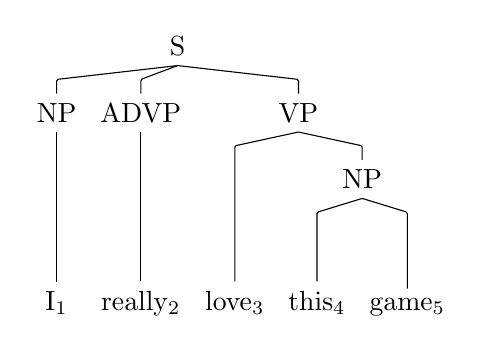
\begin{tikzpicture} [
				level distance=24pt,
				every tree node/.style={align=center,anchor=base},
				frontier/.style={distance from root=92pt},
				edge from parent/.style={draw,edge from parent path={(\tikzparentnode.south) {[rounded corners=0.5pt]-- ($(\tikzchildnode |- \tikzparentnode.south) + (0, -5pt)$) -- (\tikzchildnode)}}}
			]
			\Tree
			[.S
				[.NP I$_1$ ]
				[.ADVP really$_2$ ]
				[.VP love$_3$ [.NP this$_4$ game$_5$ ] ]
			];
		\end{tikzpicture}
		\caption{原始句法树}
		\label{fig:con-original-tree}
	\end{subfigure}
	\hfill
	\begin{subfigure}[b]{0.45\textwidth}
		\centering
		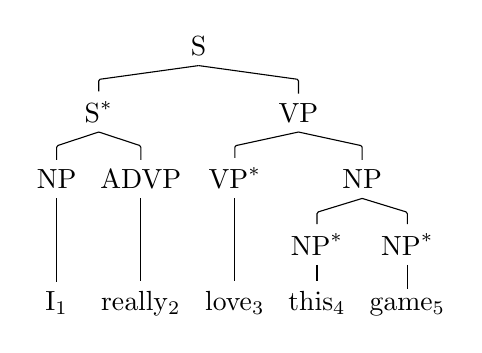
\begin{tikzpicture} [
				level distance=24pt,
				every tree node/.style={align=center,anchor=base},
				frontier/.style={distance from root=92pt},
				edge from parent/.style={draw,edge from parent path={(\tikzparentnode.south) {[rounded corners=0.5pt]-- ($(\tikzchildnode |- \tikzparentnode.south) + (0, -5pt)$) -- (\tikzchildnode)}}}
			]
			\Tree
			[.S
				[.$\textrm{S}^\ast$ [.NP I$_1$ ] [.ADVP really$_2$ ] ]
				[.VP
					[.$\textrm{VP}^\ast$ love$_3$ ]
					[.NP [.$\textrm{NP}^\ast$ this$_4$ ] [.$\textrm{NP}^\ast$ game$_5$ ] ]
				]
			];
		\end{tikzpicture}
		\caption{遵循乔姆斯基范式的左二叉化句法树}
		\label{fig:con-binaried-tree}
	\end{subfigure}
	\caption{
		成分句法树的例子.
		其中词性在这里被忽略
	}
	\label{fig:con-tree-full-figure}
\end{figure}

给定一个句子,成分句法分析旨在构建一个层次化的树结构. 如图\ref{fig:con-tree-full-figure},其中每个叶子结点是输入句子的每个词,而非终端结点作为区块(Constituents),如\texttt{$VP_{3,5}$}.

成分句法分析是自然语言处理领域一个基础但是富有挑战性的任务.
由于诸如宾州树库(Penn Treebank,PTB)、中文宾州树库(Penn Chinese Treebank,CTB)等大规模树库的标注,成分句法分析吸引了一大批研究者的关注.
同样的,句法分析输出的句法树也被证明对于大量的下游任务\cite{akoury-etal-2019-syntactically,wang-etal-2018-tree}都有用.

作为最有影响力的工作之一,\cite{collins-1997-three}概率上下文无关文法 (Probabilistic Context-Free Grammars,PCFGs)扩展到了词汇化文法(Lexicalized PCFGs).
由此开始,成分句法分析方法一直是这样的生成式模型(generative models)占据主导地位,并且其中广泛使用的Berkeley Parser采用了带隐式非终端结点标注的非词汇化概率上下文无关文法(Unlexicalized PCFGs)\cite{matsuzaki-etal-2005-probabilistic,petrov-klein-2007-improved}.
而在判别式方法(discriminative models),存在着两种主要方向.
第一种采取了以动态规划解码为基础的基于图的方法,训练时使用局部max-entropy估计\cite{kaplan-etal-2004-speed}或者全局max-margin方法\cite{taskar-etal-2004-max}.
第二类则通过基于贪婪解码或者集束搜索(beam search)产生shift-reduce这样的转移序列来构建一棵树,这种方法被称为基于转移的方法\cite{sagae-lavie-2005-classifier,zhu-etal-2013-fast}.

最近,得益于深度神经网络在上下文表示方面令人印象深刻的发展,成分句法分析取得了显著的进展.
其中,\cite{cross-huang-2016-span}的基于转移的分析器,以及\cite{stern-etal-2017-minimal}的基于图的分析器是两个具有代表性的工作.
作为判别式模型,两个分析器有很多的共同点,他们都使用了1)多层双向LSTM作为编码器;2)从双向LSTM的输出得到的minus features作为区块的表示;3)利用MLP层来为区块打分;4)max-margin的训练损失函数.
后续的大多数工作\cite{gaddy-etal-2018-whats,kitaev-klein-2018-constituency}的主要设置都和这两个分析器一样, 并且都相比传统的非神经网络模型达到了更好的准确率,这特别是得益于由在大规模无标记文本上训练的语言模型输出的上下文词表示的使用\cite{peters-etal-2018-deep,devlin-etal-2019-bert}.

然而尽管有这些显著的进展,现有的成分句法分析的研究仍然受两个相互关联的缺点困扰.
首先,解析速度(训练速度同理)很慢,并且很难满足现实系统的需要.
其次,显式的树/子树概率建模的缺失一定程度上影响来分析器输出的利用.
一方面,估计概率分布一直是自然语言处理领域的核心问题\cite{le-zuidema-2014-inside}.
另一方面,与没有上下姐的树的分值相比,树的概率可以作为一种软特征,更好的被更高层级的任务所利用\cite{jin-etal-2020-relation},且子树的边缘概率可以支持更加复杂的最小贝叶斯风险解码\cite{smith-smith-2007-probabilistic}.

事实上,\cite{finkel-etal-2008-efficient,durrett-klein-2015-neural}都通过建模树的条件概率$p(\boldsymbol{t}\mid\boldsymbol{x})$,提出了基于CRF\cite{lafferty-etal-2001-crf}的成分句法分析器.
但是,由于损失函数和梯度计算需要的Inside-Outside算法的高复杂度(尤其是Outside算法),这些模型都极端低效.
而在深度学习时代,由于以前所有的工作都直接在CPU上运行Inside-Outside算法,而让模型频繁在CPU和GPU切换所需要的时间代价是昂贵的,因此效率问题变得更加严重.

本章节通过极大拓展\cite{stern-etal-2017-minimal}的基于图的分析器,提出了一个CRF成分句法分析器.
主要的贡献在于我们为损失函数和梯度能够在GPU上能够直接计算,类似于章节\ref{cha:dep-crf},我们提出了Inside算法的批次化方法.
与此同时,我们发现Outside算法的可以通过自动的反向传播机制被高效的完成,这验证了\cite{eisner-2016-inside}出色的理论性能做,使得outside过程与Inside一样高效.
类似的,我们也批次化了CKY(Cocke–Kasami–Younger)算法,以支持高效的解码.

总体而言,我们做了如下的贡献.
\begin{itemize}
    \item 为了直接建模树和子树的概率,我们首次提出了一个快速精准的CRF成分句法分析器.
          通过批次化技术支持Inside算法和CKY算法在GPU上的直接计算,长期以来一直困扰句法分析社区的效率问题在这里被很好的解决了.

    \item 我们提出了一个两阶段的解析方法bracketing-then-labeling:先产生无标记树骨干树(bracketing)再标注标签(labeling)的解析方法,这不仅更加高效,并且达到了比一阶段解析方法稍好的性能.

    \item 我们提出了基于区块表示的一个新的打分架构,以及基于仿射注意力机制的打分方法,比minus-feature方法表现的更好.
          我们同样表明,通过更好的模型及参数设置,比如Dropout,解析的性能可以被极大提升.

    \item 在中英文的三个基准数据集上的实验表明,我们提出的两阶段解析方法在使用BERT和不使用BERT\cite{devlin-etal-2019-bert})的两种设置下,性能上达到了新的最佳水准.
          解析速度方面,我们的分析器可以达到1,000句每秒的解析速度.
\end{itemize}

\begin{figure}[tb]
    \centering
    \includegraphics [scale=1.2]{figures/con-framework.pdf}
    \caption{模型架构.}
    \label{fig:con-framework}
\end{figure}

\section{两阶段CRF解析}\label{sec:2stage-parsing}

正式地,给定一个由$n$个词组成的句子$\boldsymbol{x}=w_0,\dots,w_{n-1}$,如图~\ref{fig:con-tree-original}所示,一棵成分句法树可以表示为$\boldsymbol{t}$,其中$(i,j,l) \in \boldsymbol{t}$是一个包含$w_{i}...w_{j}$的区块,对应的句法标签为$l \in \mathcal{L}$.
一棵树同样可以被分解为两个部分,即,$\boldsymbol{t}=(\boldsymbol{y}, \boldsymbol{l})$,其中$\boldsymbol{y}$是一棵无标签树(又称为bracketed tree),而$\boldsymbol{l}$是树中所有区块的标签按一定顺序产生的标签序列.
区块$(3,5,\texttt{VP})$可以等价表示为$\texttt{VP}_{3,5}$.

为了能够适应Inside算法和CKY算法,我们用NLTK工具包\footnote{\url{https://www.nltk.org}}将原始的树转换为了遵循乔姆斯基范式(Chomsky Normal Form,CNF)的二叉树形式,如图~\ref{fig:con-binaried-tree}所示.
特别地,连续的单链产生式被压缩为了一个标签,比如$\texttt{X}_{i,j} \rightarrow \texttt{Y}_{i,j}$会被压缩为一个$\texttt{X+Y}_{i,j}$.
根据前置实验,我们在二叉化原始树的时候,采用了左二叉.
在用CKY解码获得一棵最佳的树之后,CNF树会被恢复为原来的\textit{n}-ary形式.

\subsection{模型定义}\label{sub@sec:model-definition}

在这份工作中,我们对成分句法分析采用了一个两阶段的解析框架bracketing-then-labeling.
这与传统的一阶段解析方法\cite{stern-etal-2017-minimal,gaddy-etal-2018-whats}相比,不仅简化了模型架构,同样也提升了效率.

\noindent\textbf{第一阶段:bracketing.}
给定句子$\boldsymbol{x}$,第一阶段的目标是找到一个最优的无标签树$\boldsymbol{y}$.
一棵树的分值被分解为所有包含的区块的分值.
\begin{equation} \label{eq:tree-score}
    \mathrm{s}(\boldsymbol{x},\boldsymbol{y}) = \sum\limits_{(i,j)\in \boldsymbol{y}}\mathrm{s}(i,j)
\end{equation}
对于CRF,条件概率为
\begin{equation}\label{eq:tree-prob}
    \begin{split}
        & p(\boldsymbol{y}\mid\boldsymbol{x})  = \frac{\exp({\mathrm{s}(\boldsymbol{x},\boldsymbol{y}))}}{Z(\boldsymbol{x}) \equiv \sum\limits_{\boldsymbol{y'} \in \mathcal{Y}(\boldsymbol{x})} {\exp({\mathrm{s}(\boldsymbol{x},\boldsymbol{y'}))}}}
    \end{split}
\end{equation}
其中$Z(\boldsymbol{x})$被称为partition term,$\mathcal{Y}(\boldsymbol{x})$是输入句子$\boldsymbol{x}$对应的所有合法句法树的集合.

给定所有的区块分值$\mathrm{s}(i,j)$,我们可以用CKY算法来找到一棵最优的无标签句法树$\hat{\boldsymbol{y}}$.
\begin{equation} \label{eq:tree-argmax}
    \hat{\boldsymbol{y}} = \arg\max_{\boldsymbol{y}} \mathrm{s}(\boldsymbol{x}, \boldsymbol{y}) = \arg\max_{\boldsymbol{y}} p(\boldsymbol{y} \mid \boldsymbol{x})
\end{equation}

\noindent\textbf{第二阶段:labeling.}
给定一个句子$\boldsymbol{x}$和一棵树$\boldsymbol{y}$,第二阶段独立地给每个区块$(i,j) \in \boldsymbol{y}$预测一个标签.
\begin{equation} \label{eq:label-argmax}
    \hat{l} = \arg\max_{l \in \mathcal{L}} \mathrm{s}(i,j,l)
\end{equation}
请注意训练时我们使用正确的无标签树来进行损失函数的计算.
对于一个长度为$n$的句子,所有的CNF树都包含同样$2n-1$多个的区块.
因此,这一阶段的时间复杂度为$O(n|\mathcal{L}|)$.

\noindent\textbf{时间复杂度分析.}
CKY的时间复杂度为$O(n^3)$.
因此,我们两阶段解析方法的总时间复杂度为$O(n^3+n|\mathcal{L}|)$.
相对应的,对于一阶段解析的CKY而言,算法需要为所有$n^2$个区块决定最优的标签,因此需要$O(n^3+n^2|\mathcal{L}|)$,其中$|\mathcal{L}|$通常来说都很大(比如对于表~\ref{table:con-statistics}中的英语来说为138).

\subsection{打分架构}

本章节引入了给区块和标签打分的模型架构,如图~\ref{fig:con-framework},大部分设置都遵循\cite{stern-etal-2017-minimal},除了两个重要的修改:1)针对分值计算的边界表示和仿射注意力;2)和\cite{Timothy-d17-biaffine}一样的更好的参数设置.

\noindent\textbf{模型输入.}
对于第$i$个词,其对应的输入向量$\mathbf{e}_i$是词向量和字级别表示的拼接:
\begin{equation} \label{eq:token-representation}
    \mathbf{e}_i = \mathbf{e}^{word}_i \oplus \mathrm{CharLSTM}(w_i)
\end{equation}
其中$\mathrm{CharLSTM}(w_i)$是将字序列输入到双向LSTM一样的输出向量\cite{lample-etal-2016-neural}.
以前的工作表明将词性表示用$\mathrm{CharLSTM}(w_i)$代替会带来稳定的提升\cite{kitaev-klein-2018-constituency}.
这同样简化了模型,因为不再需要额外预测词性.

\noindent\textbf{双向LSTM编码器.}
我们在输入向量上应用了三层双向LSTM以得到上下文表示.
我们分别用$\mathbf{f}_i$和$\mathbf{b}_i$来表示词$w_i$在顶层LSTM的前向和后向输出向量.

在这里,我们借用了大部分\cite{Timothy-d17-biaffine}的依存句法分析器的参数设置(参考章节\ref{sec:dep-exps}).
我们发现其中的Dropout设置对于解析性能特别关键,这和原始的实现\cite{stern-etal-2017-minimal}有两方面的不同.

首先,对于每个词$w_i$,$\mathbf{e}^{word}_i$和$\mathrm{CharLSTM}(w_i)$都作为一个整体被dropout,要么保持版本,要么称为$\mathbf{0}$向量.
如果其中一个向量被设置为了$\mathbf{0}$,则另一个会被乘以2倍作为补偿.
其次,相同LSTM层在不同的时间步(词)共享相同的dropout掩码\cite{yarin-etal-2016-dropout}.

\noindent\textbf{边界表示.}
对于每个词$w_i$,我们参考\cite{stern-etal-2017-minimal}的做法来组成上下文词向量\footnote{我们的前置实验表明$\mathbf{f}_i \oplus \mathbf{b}_{i+1}$相比于$\mathbf{f}_i \oplus \mathbf{b}_i$有稳定的提升. 可能的原因是$\mathbf{f}_i$和$\mathbf{b}_i$都使用$\mathbf{e}_i$作为输入,因此提供的信息冗余.}
\begin{equation}
    \mathbf{h}_i = \mathbf{f}_i \oplus \mathbf{b}_{i+1}
\end{equation}
$\mathbf{h}_i$的维度为800.

不同于直接应用一个单一的MLP层到$\mathbf{h}_i$上,我们发现一个词在一棵给定树的所有的区块中都必须作为其左边界或右边界.
因此,我们应用来两个MLP层来做这样的区分,并且分别获取左边界和右边界的表示向量.
\begin{equation}
    \label{mlp-borlders}
    \mathbf{r}_i^{l}; \mathbf{r}_i^{r} =\mathrm{MLP}^{l} \left( \mathbf{h}_i \right); \mathrm{MLP}^{r} \left( \mathbf{h}_i \right)
\end{equation}
$\mathbf{r}_i^{l/r}$的维度$d$为500.
正如\cite{Timothy-d17-biaffine}所指出的,MLP层缩减了$\mathbf{h}_i$的维度,并且更重要的是只保留了句法相关的信息,因此能够减轻过拟合的风险.

\noindent\textbf{仿射打分.}
给定边界表示,对于候选区块$(i,j)$,我们在左边界词$w_i$的表示和右边界词$w_j$的表示上利用仿射注意力为该区块打分.
\begin{equation} \label{eq:biaffine}
    \mathrm{s}(i,j) =  \left[
        \begin{array}{c}
            \mathbf{r}_{i}^{l} \\
            1
        \end{array}
        \right]^\mathrm{T}
    \mathbf{W} \mathbf{r}_{j}^{r}
\end{equation}
其中$\mathbf{W} \in \mathbb{R}^{d \times d}$.

计算区块标签的分值$\mathrm{s}(i,j,l)$使用的是类似的方式.
需要在$\mathbf{h}_i$上应用额外两层MLP来获取相应的边界表示$\bar{\mathbf{r}}^{l/r}_i$(维度为$\bar{d}$).
接着我们使用$|\mathcal{L}|$个Biaffine($\mathbb{R}^{\bar{d} \times \bar{d}}$)来获取所有标签的分值.
由于$|\mathcal{L}|$非常大,我们对于$\bar{\mathbf{r}}^{l/r}_i$使用了稍小的维度$\bar{d}=100$(对于${\mathbf{r}}^{l/r}_i$则是500)以减轻内存和计算负担.

\noindent\textbf{前人打分方法.}
\cite{stern-etal-2017-minimal}对双向LSTM的输出使用了minus featured方法来得到区块的表示\cite{wang-chang-2016-graph,cross-huang-2016-span},然后用MLP层得到区块的分值.
\begin{equation} \label{eq:minus-score}
    \mathrm{s}(i,j)=\mathrm{MLP}(\mathbf{h}_{i}-\mathbf{h}_{j})
\end{equation}
在实验部分我们表明我们的打分方法要明显更优越.

\subsection{训练损失函数}

对于一个训练的例子$(\boldsymbol{x},\boldsymbol{y},\boldsymbol{l})$,训练损失函数由两部分组成.
\begin{equation} \label{eq:final-loss}
    \mathit{L(\boldsymbol{x}, \boldsymbol{y}, \boldsymbol{l})} = \mathit{L}^{bracket}(\boldsymbol{x}, \boldsymbol{y}) + \mathit{L}^{label}(\boldsymbol{x}, \boldsymbol{y}, \boldsymbol{l})
\end{equation}
第一项是句子级的全局CRF损失,目的是最大化树的条件概率:
\begin{equation}\label{eq:bracket-loss}
    \begin{split}
        \mathit{L}^{bracket}(\boldsymbol{x},\boldsymbol{y})
        &= -\mathrm{s}(\boldsymbol{x}, \boldsymbol{y}) + \log Z(\boldsymbol{x})
    \end{split}
\end{equation}
其中$\log Z(\boldsymbol{x})$可以利用Inside算法在$O(n^3)$的时间复杂度内被计算.

第二项是在labeling阶段,区块级别的标准交叉熵损失函数.

\section{高效的训练和解码}
\label{sec:efficient-training-decoding}

\begin{algorithm}[tb]
  \caption{批次化的Inside算法.}
  \begin{algorithmic}[1]
    \setlength{\commentindent}{.3\textwidth}
    \setlength{\algorithmicindent}{1.5em}
    \renewcommand{\algorithmiccomment}[1]{\unskip\hfill\makebox[\commentindent][l]{$\rhd$~#1}\par}
    \LetLtxMacro{\oldalgorithmic}{\algorithmic}
    \renewcommand{\algorithmic}[1][0]{%
      \oldalgorithmic[#1]%
      \renewcommand{\ALC@com}[1]{%
        \ifnum\pdfstrcmp{##1}{default}=0\else\algorithmiccomment{##1}\fi}%
    }
    %\begin{spacing}{1.2}
    % \begin{footnotesize}
    % \STATE $\forall 0 \le i \le n ~ C_{i, i} = 0$
    % \COMMENT $\rhd$ initialization
    \STATE \textbf{define:} $S \in \mathbb{R}^{n \times n \times B}$ \COMMENT{$B$ is \#sents in a batch}
    % \STATE \hspace{\algorithmicindent}
    % \STATE \textbf{Output:} $ C_{0, n} = \log Z(\boldsymbol{x})$
    %   \COMMENT{balabala}

    \STATE \textbf{initialize:} all $S_{:, :} = 0$
    % \STATE $S_{i, i+1} = s_{i, i+1}$ \COMMENT{$w$ is 1}
    \FOR [span width]{$w = 1$ \TO $n$}
    \STATE \emph{Parallel computation on $0 \le i$,$j<n$,$~r$,$0\le b<B$}
    \STATE $S_{i, j=i+w} = \log \sum\limits_{i \le r < j} \exp \left( S_{i, r}+S_{r+1, j} \right)  + \mathrm{s}(i, j) $ \label{line:sum-product}\\
    %\textbf{batchify:} $0 \le i$; $j=i+w < n$
    \ENDFOR
    \RETURN $S_{0, n-1} \equiv \log Z(\boldsymbol{x})$
    % \end{footnotesize}
    %\end{spacing}
  \end{algorithmic}
  \label{alg:inside}
\end{algorithm}


这里我们描述如何通过批次化Inside算法和CKY算法以支持在GPU上的直接计算,来进行高效的训练和解码.
我们同样表明对于成分句法分析,复杂的Outside算法可以被自动求导机制支持的反向传播完成.

\subsection{批次化的Inside算法}

对于公式~\ref{eq:bracket-loss}里的$\log Z(\boldsymbol{x})$和特征梯度,所有以前在CRF解析上的工作\cite{finkel-etal-2008-efficient,durrett-klein-2015-neural}都显式地在CPU上进行了Inside-Outside算法的计算.
不同于线性链CRF,树状结构的CRF看起来要复杂很多.

在这里,我们发现实现一个批次化的Inside算法是可行的,如算法~\ref{alg:inside}所示.
关键的想法是将一个批次的所有实例中宽度相同的区块分值打包到一个大的张量中.
这使得我们可以通过高效的大规模张量操作进行计算和合并.
由于对所有的$0 \le i$,$j<n$,$~r$,$0\le b<B$而言,在GPU上的计算都是并行的,因此算法仅需要$O(n)$步.
我们的代码会给出更多的技术细节.

\subsection{Outside算法的替代:反向传播}

传统上,Outside算法被认为对于子树边缘概率和特征梯度的计算是不可或缺的.
事实上,Outside算法通常至少要两倍慢于Inside算法.
而Outside算法的批次化也要复杂的多.
幸运的是,这个问题在深度学习时代被很好的解决了,基于自动求导机制支持的反向传播可以方便的获取梯度.
\cite{eisner-2016-inside}提出了理论上关于反向传播和Outside过程的等价性证明,和章节~\ref{cha:dep-crf}一样,我们给出的简化版本证明在附录~\ref{sec:outside-backprop}.
由于我们在前向过程使用来批次化的Inside算法,因此反向传播过程也是通过大规模张量并行计算的,可以视为同样高效.

值得注意的是通过用区块分值$\mathrm{s}(i,j)$对$\log Z(\boldsymbol{x})$求偏导(同样由自动的反向传播完成),我们可以自然的得到区块$(i,j)$的边缘概率,也就是梯度.
\begin{equation} \label{eq:partial-derivative}
    p((i, j)\mid\boldsymbol{x}) = \frac{\partial \log Z(\boldsymbol{x})}{\partial \mathrm{s}(i, j)}
\end{equation}
边缘概率在很多下游任务都可以作为一种很有用的软特征.
更多细节可以参考\cite{eisner-2016-inside}.

\subsection{解码}

正如上面提到的,解析过程中,我们应用CKY算法来获取一棵最佳的句法树,如公式~\ref{eq:tree-argmax}所示.
和Eisner算法一样,CKY算法和成分句法分析的Inside算法几乎一样,除了其中的sum-product被替换为了max product(参考算法~\ref{alg:inside}的行~\ref{line:sum-product}),因此可以被同样高效的批次化.
为了进行MBR解码,我们直接将区块分值$\mathrm{s}(i,j)$换成式~\ref{eq:tree-score}和式~\ref{eq:tree-argmax}的边缘概率$p((i,j)\mid\boldsymbol{x})$.
然而,我们发现这在成分句法上带来了很微弱的提升.

\begin{table}[tb!]
    \centering
    \caption{数据统计,包含句子数和标签树.
        对于``\#labels'',我们列出了原始树和CNF树对应的标签数.}
    \begin{tabular}{lrrr|ccc}
        \toprule
               & \multirow{2}{*}{\#Train} & \multirow{2}{*}{\#Dev} & \multirow{2}{*}{\#Test} & \multicolumn{2}{c}{\#labels}       \\
               &                          &                        &                         & original                     & CNF \\[1pt]
        \midrule
        % \\[-8pt]
        PTB    & 39,832                   & 1,700                  & 2,416                   & 26                           & 138 \\
        CTB5.1 & 18,104                   & 352                    & 348                     & 26                           & 162 \\
        CTB7   & 46,572                   & 2,079                  & 2,796                   & 28                           & 265 \\
        \bottomrule
    \end{tabular}
    \label{table:con-statistics}
\end{table}

\section{实验}
\label{sec:con-experiments}
\noindent\textbf{数据.}
我们主要在三个中文和英文的数据集上进行实验.
前两个数据集,即PTB和CTB5.1,是句法分析社区中比较常用的两个数据集.
我们遵循了传统的train/dev/test数据的分割.
考虑到CTB5.1的dev/test都只有大约350句,为了得到更加稳定一致的结果,我们同样在更大的CTB7数据上进行了实验,相关的数据分割设置参考了官方手册建议.
表~\ref{table:con-statistics}列出了相关数据的统计信息.
可以看到CNF转换引入了很多新的区块标签,其中大部分(大约75\%)是源于连续单链的折叠过程.

\noindent\textbf{评价.}
正如前面提到的,在解析之后,我们将最佳的CNF树转化为了\textit{n}-ary树再进行评价.
这里有必要提及一些有用的细节.
由于解码算法没有相应的约束,预测的最佳CNF树可能包含很多不合法的产生式.
以图~\ref{fig:con-binaried-tree}为例,模型可能输出$\texttt{VP}_{3,5} \rightarrow \texttt{PP}^{\ast}_{3,3} ~ \texttt{NP}_{4,5}$,其中 $\texttt{VP}$和$\texttt{PP}^{\ast}$是不兼容的.
在\textit{n}-ary后处理过程中,我们直接忽略了``$\mathtt{\ast}$''符号之前具体的字符串$\texttt{PP}$.
有鉴于此,如果解码的时候增加一定的约束,结果有可能进一步提高,这里我们留待后续的工作.

我们使用了标准的区块级别的准确率、召回率和F值(P/R/F)作为评价指标,并使用\texttt{EVALB}工具\footnote{\url{https://nlp.cs.nyu.edu/evalb}}来评价.
特别地,一个诸如$\texttt{VP}_{3,5}$的预测区块如果出现在了正确树中,那就被认为是正确的.\footnote{
    由于一些研究者可能会实现他们自己的评价叫门,为了比较的公平,需要澄清一些细节:
    1)一些诸如\{-NONE-\}的空区块在预处理的时候被移除了.
    2)评价的时候作为根结点的区块(英语里是\{TOP,S1\},中文里是空字符串) 被忽略了.
    3)包含一些例如\{:,``,'',.,?,!\}这些标点的区块也被忽略了. 请注意中文标点会作为正常的字符被评价.
    4)一些在同一集合中的标签,例如\{ADVP,PRT\},被认为是等价的.}

\noindent\textbf{参数设置.}
我们直接采用\cite{Timothy-d17-biaffine}的依存句法分析器里面的大部分参数设置,没有进一步的改动.
唯一的区别是我们用了CharLSTM词表示,而非词性embedding.
CharLSTM里自向量、词向量以及CharLSTM输出向量的维度分别为50、100和100.
所有Dropout的比率为0.33.
一个批次数据的大小约为5,000个词.
训练过程持续至多不超过1,000次迭代,并且如果Dev数据上的最高结果连续100次不提示,那么训练就会提前停止.

\begin{table*}[tb!]
    % \setlength{\tabcolsep}{8.6pt}
    \centering
    \begin{tabularx}{\textwidth}{lccccccccc}
        \toprule
                               & \multicolumn{3}{c}{PTB} & \multicolumn{3}{c}{CTB5.1} & \multicolumn{3}{c}{CTB7}                                                                                                       \\
        % \cmidrule(lr){2-4}\cmidrule(lr){6-8}\cmidrule(lr){10-12}
                               & P                       & R                          & F                        & P              & R              & F              & P              & R              & F              \\
        \midrule
        % \\[-8pt]
        Max-margin (one-stage) & 93.70                   & 93.73                      & 93.72                    & 90.60          & 90.48          & 90.54          & 86.85          & 86.08          & 86.47          \\
        CRF (one-stage)        & 93.44                   & 93.75                      & 93.60                    & \textbf{91.08} & 90.98          & \textbf{91.03} & 87.10          & 86.75          & 86.93          \\[3pt]
        CRF (two-stage)        & \textbf{93.77}          & \textbf{93.96}             & \textbf{93.86}           & 90.91          & 91.09          & 91.00          & \textbf{87.27} & \textbf{87.00} & \textbf{87.13} \\
        \qquad w/o MBR         & 93.75                   & 93.85                      & 93.80                    & 90.93          & \textbf{91.10} & 91.02          & 87.21          & 86.89          & 87.05          \\
        % \hline
        \qquad minus features  & 93.40                   & 93.35                      & 93.37                    & 90.60          & 90.51          & 90.56          & 86.96          & 86.24          & 86.60          \\
        \qquad vanilla dropout & 92.80                   & 93.00                      & 92.90                    & 89.68          & 89.68          & 89.68          & 85.55          & 85.54          & 85.54          \\

        \bottomrule
    \end{tabularx}
    \caption{dev数据上的结果. 所有模型都使用了随机初始化的词向量.}
    \label{table:con-dev}
\end{table*}

\subsection{Dev数据上的模型比较}

We conduct the model study on dev data from two aspects: 1) CRF vs. max-margin training loss; 2) two-stage vs. one-stage parsing.
The first three lines of
Table~\ref{table:con-dev} shows the results.
The three models use the same scoring architecture and parameters.
Following previous practice \cite{stern-etal-2017-minimal},one-stage models use only scores of labeled constituents $\mathrm{s}(i,j,l)$.
%on the dev data,including the max-margin and our CRF approach.
% \footnote{We perform MBR decoding on all datasets for the CRF approach and the improvement brought by MBR is very slight. We ignore the exhibition of the results without MBR due to space limitation.}
% For fairness,we retain the biaffine scoring in the max-margin method.
In order to verify the effectiveness of the two-stage parsing,we also list the results of ``CRF (one-stage)'',which directly scores labeled constituents.
\begin{equation} \label{eq:tree-label-score}
    \mathrm{s}(\boldsymbol{x},\boldsymbol{y},\boldsymbol{l}) =
    %\sum_{(i,j)\in \boldsymbol{y}} {\mathrm{s}(i,j) +
    \sum_{(i,j,l) \in (\boldsymbol{y}, \boldsymbol{l})} \mathrm{s}(i,j,l)
\end{equation}
As discussed in the last paragraph of Section \ref{sub@sec:model-definition},the inside and CKY算法s become a bit more complicated for the one-stage parser that two-stage.

From the first two rows,we can see that
under the one-stage parsing framework,the CRF loss leads to similar performance on English
but consistently outperforms the max-margin loss by about 0.5 F-score on both Chinese datasets.
The max-margin loss has one extra hyper-parameter,namely the margin value,which is set to 1 according to preliminary results on English and not tuned on Chinese for simplicity.
We suspect that the performance on Chinese with max-margin loss may be improved with more tuning.
%First,we compare the one-stage CRF approach,with widely used max-margin loss.
%The results of max-margin are very close to that of CRF in English.
%But on Chinese,CRF outperforms the max-margin consistently by about 0.5.
%This is partly because we do not tune hyper-parameters for max-margin specifically.
%We believe that max-margin still has the potential to catch up with our CRF approach with a proper setting.
% the CRF parsing span and label together is named as ``CRF w/ label''. its architecture is identical to ``Max-margin'' but loss function.
Overall,we can conclude that the two training loss settings achieve very close performance,and CRF has an extra advantage of probabilistic modeling.

Comparing the second and third rows,the two CRF parsers achieve nearly the same performance on CTB5.1 and the two-stage parser achieves modest improvement over the one-stage parser by about 0.2 F-score on both PTB and CTB7.
Therefore,we can conclude that our proposed two-stage parsing approach is superior in simplicity and efficiency (see Table~\ref{table:speed}) without hurting performance.

\begin{table}[tb!]
  \setlength{\tabcolsep}{15pt}
  \centering
  \caption{PTB的Test数据上的解析速度比较.}
  \begin{tabular}{lr}
    \toprule
                                                          & Sents/sec     \\
    \midrule
    % \\[-8pt]
    \citet{petrov-klein-2007-improved}  (Berkeley Parser) & 6             \\
    \citet{zhu-etal-2013-fast} (ZPar)                     & 90            \\
    \citet{stern-etal-2017-minimal}                       & 76            \\
    \citet{shen-etal-2018-straight}                       & 111           \\
    \citet{kitaev-klein-2018-constituency}                & 332           \\
    \citet{gomez-rodriguez-vilares-2018-constituent}      & 780           \\[3pt]
    \textsc{Crf} (one-stage)                              & 990           \\
    \textsc{Crf} (two-stage) w/ MBR                       & 743           \\
    \textsc{Crf} (two-stage) w/o MBR                      & \textbf{1092} \\
    \textsc{Crf2o} (two-stage) w/ MBR                     & 598           \\
    \textsc{Crf2o} (two-stage) w/o MBR                    & 864           \\

    \bottomrule
  \end{tabular}
  \label{table:speed}
\end{table}
\begin{table*}[tb]
  \centering
  \caption{Test数据的结果.}
  \begin{tabularx}{\textwidth}{lccccccccc}
    \toprule
                                                     & \multicolumn{3}{c}{PTB}  & \multicolumn{3}{c}{CTB5.1} & \multicolumn{3}{c}{CTB7}                                                                                                                                     \\
                                                     & $\mathrm{P}$             & $\mathrm{R}$               & $\mathrm{F}_1$           & $\mathrm{P}$             & $\mathrm{R}$             & $\mathrm{F}_1$           & $\mathrm{P}$   & $\mathrm{R}$   & $\mathrm{F}_1$ \\
    \midrule
    % \\[-8pt]
    % \multicolumn{4}{l}{\textbf{Random word embeddings}} \\
    % \citet{liu-zhang-2017-shift}                     &         92.1\textcolor{white}{0}   &         91.3\textcolor{white}{0}   &         91.7\textcolor{white}{0}   &&         85.9\textcolor{white}{0}   &         85.2\textcolor{white}{0}   &         85.5\textcolor{white}{0}   &&         -      & -              & -              \\
    \citet{stern-etal-2017-minimal}                  & 92.98                    & 90.63                      & 91.79                    & -                        & -                        & -                        & -              & -              & -              \\
    % \citet{liu-2018-improving}                       &         -      &         -      &         91.2   &&         -      &         -      &         84.1   &&         -      & -              & -              \\
    % \citet{fried-klein-2018-policy}                       &         -      &         -      &         92.2   &&         -      &         -      &         87.0   &&         -      & -              & -              \\
    % \citet{stern-etal-2017-effective}                &         92.57   &          92.56   &         92.56  \\
    \citet{gaddy-etal-2018-whats}                    & 92.41                    & 91.76                      & 92.08                    & -                        & -                        & -                        & -              & -              & -              \\
    \citet{kitaev-klein-2018-constituency}           & 93.90                    & 93.20                      & 93.55                    & 88.09                    & 86.78                    & 87.43                    & -              & -              & -              \\
    \citet{gomez-rodriguez-vilares-2018-constituent} & -                        & -                          & 90.0\textcolor{white}{0} & -                        & -                        & 84.4\textcolor{white}{0} & -              & -              & -              \\
    \citet{shen-etal-2018-straight}                  & 92.0\textcolor{white}{0} & 91.7\textcolor{white}{0}   & 91.8\textcolor{white}{0} & 86.6\textcolor{white}{0} & 86.4\textcolor{white}{0} & 86.5\textcolor{white}{0} & -              & -              & -              \\
    \citet{teng-zhang-2018-two} %(w/ pretrained)
                                                     & 92.5\textcolor{white}{0} & 92.2\textcolor{white}{0}   & 92.4\textcolor{white}{0} & 87.5\textcolor{white}{0} & 87.1\textcolor{white}{0} & 87.3\textcolor{white}{0} & -              & -              & -              \\

    \citet{vilares-etal-2019-better}                 & -                        & -                          & 90.60                    & -                        & -                        & 85.61                    & -              & -              & -              \\
    \citet{zhou-zhao-2019-head} w/ pretrained        & 93.92                    & 93.64                      & 93.78                    & 89.70                    & 89.09                    & 89.40                    & -              & -              & -              \\[3pt]
    \textsc{Crf}                                     & 93.84                    & 93.58                      & 93.71                    & 89.18                    & 89.03                    & 89.10                    & 87.66          & 87.21          & 87.43          \\
    \textsc{Crf2o}                                   & 94.06                    & 93.84                      & 93.95                    & 89.04                    & 88.68                    & 88.86                    & 87.86          & 87.40          & 87.63          \\
    \textsc{Crf} w/ pretrained                       & 94.23                    & 94.02                      & 94.12                    & 89.71                    & \textbf{89.89}           & \textbf{89.80}           & 88.84          & 88.36          & 88.60          \\
    \textsc{Crf2o} w/ pretrained                     & \textbf{94.29}           & \textbf{94.15}             & \textbf{94.22}           & \textbf{89.97}           & 89.47                    & 89.72                    & \textbf{88.95} & \textbf{88.56} & \textbf{88.76} \\[1pt]
    \midrule
    \\[-20pt]
    \citet{kitaev-klein-2018-constituency} w/ ELMo   & 95.40                    & 94.85                      & 95.13                    & -                        & -                        & -                        & -              & -              & -              \\
    \citet{kitaev-etal-2019-multilingual} w/ BERT    & 95.73                    & 95.46                      & 95.59                    & 91.96                    & 91.55                    & 91.75                    & -              & -              & -              \\[3pt]
    \textsc{Crf} w/ BERT                             & \textbf{95.85}           & \textbf{95.53}             & \textbf{95.69}           & 92.51                    & 92.04                    & 92.27                    & 91.73          & \textbf{91.38} & 91.55          \\
    \textsc{Crf2o} w/ BERT                           & 95.73                    & 95.45                      & 95.59                    & \textbf{92.75}           & \textbf{92.18}           & \textbf{92.47}           & \textbf{91.93} & 91.31          & \textbf{91.62} \\
    \bottomrule
  \end{tabularx}
  \label{table:con-test}
\end{table*}



\subsection{dev数据上的消融实验}

To gain insights into the contributions of individual components in our proposed framework,
we then conduct the ablation study by undoing one component at a time. % to \cite{stern-etal-2017-minimal}.
Results are shown in the bottom four rows of Table~\ref{table:con-dev}.

\noindent\textbf{MBR解码的影响.}
By default,we employ CKY decoding over marginal probabilities,a.k.a. MBR decoding.
The ``w/o MBR'' row presents the results of performing decoding over span scores.
Such comparison is very interesting since it is usually assumed that MBR decoding is theoretically superior to vanilla decoding.
However,the results clearly show that
the two decoding methods achieve nearly identical performance.

\noindent\textbf{打分架构的影响.}
In order to measure the effectiveness of our new scoring architecture,we revert the biaffine scorers to the ``minus features'' method adopted by \cite{stern-etal-2017-minimal} (refer to Equation~\ref{eq:minus-score}).
It is clear that our proposed scoring method is superior to the widely used minus-feature method,and
achieves a consistent and substantial improvement of about 0.5 F-score on all three datasets.

\noindent\textbf{Dropout策略的影响.}
We keep other model settings unchanged and only replace the dropout strategy borrowed from \cite{Timothy-d17-biaffine} with the vanilla dropout strategy adopted by \cite{stern-etal-2017-minimal}.
This leads to a very large and consistent performance drop of 0.96,1.39 and 1.59 in F-score on the three datasets,respectively.
\cite{kitaev-klein-2018-constituency} replaced 双向LSTMs with a self-attention encoder in \cite{stern-etal-2017-minimal} and achieved a large improvement of 1.0 F-score by separating content and position attention.
Similarly,this work shows that the 双向LSTM-based parser can be very competitive with proper parameter settings.

\subsection{速度比较}
Table~\ref{table:speed} compares different parsing models in terms of parsing speed.
Our models are both run on a machine with Intel Xeon E5-2650 v4 CPU and Nvidia GeForce GTX 1080 Ti GPU.
Berkeley Parser and ZPar are two representative non-neural parsers without access to GPU.
\cite{stern-etal-2017-minimal} employ max-margin training and perform CKY-like decoding on CPUs.
\cite{kitaev-klein-2018-constituency} use a self-attention encoder and perform decoding using Cython for acceleration.


We can see that our one-stage CRF parser is much more efficient than previous parsers by directly performing decoding on GPU.
Our two-stage parser can parse 1,092 sentences per sentence,which is three times faster than \cite{kitaev-klein-2018-constituency}.
Of course,it is noteworthy that those parsers \cite{stern-etal-2017-minimal,kitaev-klein-2018-constituency} may be equally efficient by adopting our batchifying techniques.

The parser of \cite{gomez-rodriguez-vilares-2018-constituent} is also very efficient by treating parsing as a sequence labeling task. However,the parsing performance is much lower,as shown in Table~\ref{table:test}.

The two-stage parser is only about 10\% faster than the one-stage counterpart. The gap seems small considering the significant difference in time complexity as discussed (see Section~\ref{sub@sec:model-definition}).
The reason is that the two parsers share the same encoding and scoring components,which consume a large portion of the parsing time.

Using MBR decoding requires an extra run of the inside and back-propagation algorithms for computing marginal probabilities,and thus is less efficient.
As shown in Table~\ref{table:con-dev},the performance gap is very slight between w/ and w/o MBR.

\subsection{Test数据上的结果和比较}
%The results of English and Chinese on the test data is shown in
Table~\ref{table:test} shows the final results on the test datasets under two settings,i.e.,w/o and w/ ELMo/BERT.

Most previous works do not use pretrained word embedding but use randomly initialized ones instead,except for \cite{zhou-zhao-2019-head},who use Glove for English and structured skip-gram embeddings.
For pretrained word embeddings,we use Glove (100d) %\cite{pennington-etal-2014-glove}
for English PTB\footnote{\url{https://nlp.stanford.edu/projects/glove}},
and adopt the embeddings of \cite{li-etal-2019-attentive} trained on Gigaword 3rd Edition for Chinese.
% Looking at the results of using pretrained word embeddings,
It is clear that our parser benefits substantially from the pretrained word embeddings.\footnote{
    We have also tried the structured skip-gram embeddings kindly shared by \cite{zhou-zhao-2019-head} for Chinese,and achieved similar performance by using our own embeddings.
}

We also make comparisons with recent related works on constituency parsing,as discussed in Section~\ref{sec:relwork}.
We can see that our 双向LSTM-based parser outperforms the basic \cite{stern-etal-2017-minimal} by a very large margin,mostly owing to the new scoring architecture and better dropout settings.
Compared with the previous state-of-the-art self-attentive parser \cite{kitaev-klein-2018-constituency},
our parser achieves an absolute improvement of 0.16 on PTB and 1.67 on CTB5.1 without any language-specific settings.

The CTB5.1 results of \cite{zhou-zhao-2019-head} is obtained by rerunning their released code using predicted POS tags.
We follow their descriptions\footnote{\url{https://github.com/DoodleJZ/HPSG-Neural-Parser}} to produce the POS tags.
% predicted by the Stanford tagger \cite{toutanova-etal-2003-feature}.
It is noteworthy that their reported results accidentally use gold POS tags on CTB5.1,which is confirmed after several turns of email communication. We are grateful for their patience and help.
We reran their released code using gold POS tags,and got 92.14 in F-score on CTB5-test,very close to the results reported in their paper.
Our parser achieves 92.66 F-score with gold POS tags.
Another detail about their paper should be clarified: for dependency parsing on Chinese,they adopt two different data split settings,both using Stanford dependencies 3.3.0 and gold POS tags.

The bottom three rows list the results under the setting of using ELMo/BERT.
We use bert-large-cased\footnote{\url{https://github.com/huggingface/transformers}} (24 layers,1024 dimensions,16 heads) for PTB following \cite{kitaev-etal-2019-multilingual},and bert-base-chinese (12 layers,768 dimensions,12 heads) for CTB.
It is clear that using BERT representations can help our parser by a very large margin on all datasets. %,which is consistent with previous works.
Our parser also outperforms the multilingual parser of \cite{kitaev-etal-2019-multilingual},which uses extra multilingual resources.
In summary,we can conclude that our parser achieves state-of-the-art performance in both languages and both settings.

\section{本章小结}\label{sec:con-conclusions}

In this work,we propose a fast and accurate neural CRF constituency parser. We show that the inside and CKY算法s can be effectively batchified to accommodate direct large tensor computation on GPU,leading to dramatic efficiency improvement.
The back-propagation procedure is equally efficient and erases the need for the Outside算法 for gradient computation.
Experiments on three English and Chinese benchmark datasets lead to several promising findings.
First,the simple two-stage bracketing-then-labeling approach is more efficient than one-stage parsing without hurting performance.
Second,our new scoring architecture achieves higher performance than the previous method based on minus features.
Third,the dropout strategy we introduce can improve parsing performance by a large margin.
Finally,our proposed parser achieves new state-of-the-art performances with a parsing speed of over 1,000 sentences per second.

\chapter{基于变分推断的TreeCRF加速}
\label{cha:vi}

本章节在章节~\ref{cha:dep-crf}和~\ref{cha:con-crf}提出的高阶句法分析器的基础上,尝试利用基于平均场变分推断来近似得到树的后验概率,并与精确推断的CRF相比较.
我们在依存句法和成分句法的中英文常见的5个基准数据集上做了实验,并对比了加入BERT之后的效果.
结果表明,我们采用的变分推断近似方法不仅从准确率上可以与章节~\ref{cha:dep-crf}和~\ref{cha:con-crf}里提出的二阶基于图的解析器相匹敌,并且训练和测试的速度要远远快于二阶CRF解析器.

\section{引言}\label{sec:vi-intro}
近年来句法分析领域有了长足的进步.
研究者针对句法分析任务提出了一系列的方法 \citep{dozat-etal-2017-biaffine,gomez-rodriguez-vilares-2018-constituent,ji-etal-2019-graph,zhang-etal-2020-fast,wei-etal-2020-span},将英语基准数据集宾州树库(Penn Treebank, PTB)的准确率刷新到了很高的水平.
本章中我们主要关注于基于图的句法分析方法.

基于图的方法选择将一棵句法树分解为多个部分,然后分别打分,组成树的分值,并训练模型使得能够找到分值最大的句法树.
其中最简单的一阶方法让树中的每个变量都互相独立.
在深度学习时代之前,一阶方法通常需要结合结构化学习 \citep{mcdonald-etal-2005-online,koo-etal-2007-structured,taskar-etal-2004-max}.
得益于深度神经网络的强大上下文建模能力,近期的一些工作通常基于更简单的训练方法,其中\citet{dozat-etal-2017-biaffine}(Biaffine Parser)提出一个简单的基于头选择目标的解析器,训练时最大化每条弧的头的概率.
\citet{gaddy-etal-2018-whats}则提出一个基于二分类目标的成分句法分析方法,训练模型判断每个可能位置是否组成组块.
由于其高效率,并且取得了不逊色于结构化学习方法的结果 \citep{zhang-etal-2019-empirical,falenska-kuhn-2019-non},这些方法是目前最为流行的句法分析方法.

与此对应的,研究者通常也尝试更多结构化约束引入神经网络模型中.
一方面利用TreeCRF、Max Margin \citep{ma-hovy-2017-neural,falenska-kuhn-2019-non,stern-etal-2017-minimal}等结构化学习算法来全局最大化句法树的概率.
另一方面,则是尝试利用高阶特征,建模兄弟、祖父等子树结构 \citep{mcdonald-pereira-2006-online,koo-collins-2010-efficient}.
我们在章节~\ref{cha:dep-crf}和章节~\ref{cha:con-crf}的工作证明,在神经网络模型中,引入结构化学习给句法分析任务会给带来了一定的提升.
在依存句法分析中我们还进一步尝试了二阶兄弟特征的高阶句法分析,是依存分析的结果超越了一系列前人的工作,达到了最佳水平.

尽管在神经网络上被证明有效,高阶结构化学习方法的一些固有缺陷限制了其应用.
由于需要精确推断得到树概率,这需要$O(n^3)$的时间复杂度,因此大大慢于一阶方法.
此外,如果进一步考虑其他高阶特征,例如共同父亲等等,这可能会导致动态规划结构难以设计,或者算法复杂度难以忍受.

考虑到这种限制,因此,在本章中我们参考前人的一些工作 \citep{smith-eisner-2008-dependency,wang-etal-2019-second,wang-tu-2020-second},在利用高阶特征的同时,尝试用平均场变分推断(Mean Field Variational Inference, MFVI)方法来近似获得后验概率.
在本章中,我们在依存句法分析和成分句法分析这两个句法分析任务上尝试了应用基于变分推断的近似学习算法.
针对依存解析和成分解析两种任务的特性,我们分别在依存句法的变分推断中参考\cite{wang-tu-2020-second}引入了头选择的结构约束,而在成分句法中则采用了二分类的学习目标.
我们发现近似算法在获取了和精确推断接近的准确率的同时,解析速度能够大大提高.

% 近似方法 \citep{smith-eisner-2008-dependency,gormley-etal-2015-approximation},并使用$AD^3$ \citep{martins-etal-2011-dual,martins-etal-2013-turning}来进行解码.
总体而言,我们在本章节的工作如下:
\begin{itemize}
  \item 我们提出在句法分析任务上应用引入二阶特征的变分推断方法近似得到后验概率来进行结构化学习,并和前述章节的精确推断方法做了比较.
  \item 针对依存句法分析和成分句法分析任务的特性,我们分别探索了基于头选择的变分推断方法和基于二分类的变分推断方法用到两种句法分析任务上.
  \item 我们在中文和英文数据上做了实验,在加入BERT之后,我们的变分推断方法在一些数据集上达到了新的最佳结果,
        并且,在依存和成分句法分析上分别可以达到到1,126句和905句每秒的解析速度.
\end{itemize}

\section{基于MFVI的二阶模型}\label{sec:vi-2o-approach}

本章在章节~\ref{cha:dep-crf}以及章节~\ref{cha:con-crf}的基础上,分别设计了一个基于变分推断的二阶依存句法和成分句法模型.
本章保持了前面章节提出的二阶模型架构,区别是用MFVI近似算法代替了精确推断的TreeCRF方法,从而大大降低了复杂度.

\subsection{模型定义}\label{sec:vi-model-definition}

我们保持了和精确推断模型一致的两阶段解析策略.

\noindent\textbf{第一阶段}:给定输入句子$\boldsymbol{x}$,目标是找到一棵最优(概率最高)的无标签树$\boldsymbol{y}=\arg\max_{\boldsymbol{y}^{\prime}}p(\boldsymbol{x},\boldsymbol{y}^{\prime})$.
在精确推断方法中,为了得到树概率,我们需要通过$O(n^3)$复杂度的Inside算法计算配分项$Z(\boldsymbol{x})\equiv\sum_{\boldsymbol{y}^{\prime}\in\mathcal{Y}}\mathrm{s}(\boldsymbol{x},\boldsymbol{y}^{\prime})$,来对分值$\mathrm{s}(\boldsymbol{x},\boldsymbol{y})$全局归一化,因此十分低效.

在本节我们提出利用高效的基于平均场理论的变分推断法(Mean Field Variational Inference, MFVI)来近似得到后验概率的方法.
MFVI假设句法树$\boldsymbol{y}$每个位置的变量相互独立,因此可以在线性时间内通过不断迭代得到后验概率的近似分布$Q(\cdot)$.
关于MFVI的通用更新公式以及相关推导见附录~\ref{appendix:mfvi-derivation}.
根据任务目标的不同,我们为依存句法和成分句法分别设计了两种不同的因子图,以及相应的更新方法.

\noindent\textbf{第二阶段}:我们的目标是为预测的无标签树$\boldsymbol{x}$的每个部分预测标签,得到标签序列$\boldsymbol{l}$.
依存树上$\boldsymbol{l}$被分解为每条弧的标签,成分树上$\boldsymbol{l}$由每个组块的标签组成.
我们采取和前述一样的方法,以贪婪解码的方式,为无标签依存句法树的每条弧$i\rightarrow j$找到一个分值最大的标签,成分句法树的每个组块$(i,j)$找到一个最优的标签.

\subsection{二阶子树打分}

具体而言,给定一个句子$\boldsymbol{x}$,我们的模型将对应的词向量输入到3层双向LSTM来计算每个位置的上下文表示,其中第$i$个词的输出为$\mathbf{h}_i$.
接着,我们利用$\mathbf{h}_i$对句法树的每个子结构进行打分.
对于依存句法,我们利用公式~\ref{eq:biaffine}得到每条弧$i\rightarrow j$的分值$\mathrm{s}(i\rightarrow j)$,对于成分句法,我们用公式~\ref{eq:con-biaffine}得到每个组块$(i, j)$的分值$\mathrm{s}(i, j)$.

我们在变分推断方法中还引入了二阶子树特征.
其中,依存句法中,我们采用了和章节~\ref{cha:dep-crf}一样的兄弟子树结构.
我们利用公式~\ref{eq:triaffine}得到兄弟子树$i\rightarrow \{k,j\}$的分值$\mathrm{s}(i\rightarrow\{k,j\})$,其中$k$是$j$的兄弟并且两者的父亲均为$i$.
成分句法中,参考章节~\ref{cha:con-crf},我们利用公式~\ref{eq:con-triaffine}得到$\mathrm{s}(i,k,j)$,代表由$(i,k)$和$(i,j)$两个组块构成的子树$(i,k,j)$的分值,$k$和$j$分别是两个组块的右边界位置,并且左边界均为$i$.

对于标签的分值,我们利用Biaffine结构,分别得到依存树每条弧上的每个标签的分值$\mathrm{s}(i\rightarrow j,l)$,以及成分句法树每个组块上的每个标签的分值$\mathrm{s}((i,j),l)$.

\subsection{依存句法的MFVI方法}\label{sec:dep-vi}

\begin{figure}[tb!]
  \centering
  \begin{subfigure}[b]{0.8\textwidth}
    \centering
    \includegraphics[scale=1]{figures/dep-factors.pdf}
    \caption{依存句法模型的因子图}
    \label{fig:dep-factors}
  \end{subfigure}
  \begin{subfigure}[b]{0.8\textwidth}
    \centering
    \includegraphics[scale=1]{figures/con-factors.pdf}
    \caption{成分句法模型的因子图}
    \label{fig:con-factors}
  \end{subfigure}
  \caption{一个例句和其依存/成分句法模型对应的因子图,我们在例句上方标出了对应的正确无标签依存句法树和成分句法树,其中成分句法树进行了左二叉化.
    灰色虚线圆圈代表被屏蔽的变量.
    图中标出了所有的一阶(红色)因子,为了简洁起见,对于二阶因子,依存句法图中我们只标出了涉及弧$3\rightarrow 4$的兄弟(绿色)因子,成分句法图中只标出了和组块$(3, 4)$连接的二阶(蓝色)因子.}
  \label{fig:vi-factors}
\end{figure}

目前广泛使用的一阶局部模型(对应于章节~\ref{cha:dep-crf}的\textsc{Loc}方法,这里我们称为\textsc{Loc}$_{dep}$)在训练的时候采用了头选择(head selection)的训练损失函数,要求句子中除了根结点之外的每个词有且仅有一个头.
和\citet{wang-tu-2020-second}一样,我们选择在依存句法对应变分推断方法中引入头选择约束,相应的因子图设计见图~\ref{fig:dep-factors}.
对于每个位置$j$,我们定义变量取值$y_j\in \{0,1,\cdots,i\neq j,\cdots,n\}$,代表词$w_j$的可能的头索引.

具体地,对于每个变量$y_j$,一阶的势函数定义为
\begin{equation}
  \label{eq:dep-1o-potential}
  \psi_j(y_j)=\exp(s(y_j\rightarrow j))
\end{equation}
$s(y_j\rightarrow j)$是弧$y_j\rightarrow j$对应的分值,由公式~\ref{eq:biaffine}计算得到.

对于包含两个变量$y_{j}$和$y_{k}$的二阶因子,对应的势函数定义为
\begin{equation}
  \label{eq:2o-dep-potential}
  \psi_{j,k}(y_j,y_k)=\left\{
  \begin{array}{rcl}
    \exp \mathrm{s}(y_j\rightarrow \{k,j\}) &  & {y_j=y_k}   \\
    1                                       &  & {otherwise}
  \end{array}
  \right.
\end{equation}
$s(y_j\rightarrow \{k,j\})$是兄弟子树$y_j\rightarrow \{k,j\}$的分值,由公式~\ref{eq:triaffine}计算得到.
需要注意的是这里的兄弟$k$和二阶TreeCRF不同,并不需要一定和$j$邻近 \citep{smith-eisner-2008-dependency}.
我们要求子树$y_j\rightarrow \{k,j\}$中没有环存在,即有$k\neq {0,j,y_j}$.

MFVI迭代式地更新近似分布$Q(\cdot)$,来最小化其与真实分布$P(\cdot)$的KL散度.
依存句法模型的迭代更新公式如下 \citep{wang-tu-2020-second}:
\begin{equation}
  \label{eq:mfvi-dep}
  Q_{j}^{(t)}(i)\propto \exp\left(s(i\rightarrow j) +\sum_{k\neq i,j} Q_{k}^{(t-1)}(i)\cdot s(i\rightarrow {k,j}) \right)
\end{equation}
后验分布$Q_j^{(0)}(i)$初始化为一阶势函数的值$\psi_j(i)$.
每次迭代时,我们都会将$Q_j^{(t)}(\cdot)$的值在所有可能的头取值上进行归一化.
经过$T$次迭代后,我们得到最终的近似后验分布$Q_j^{(T)}(\cdot)$.

\subsection{成分句法的MFVI方法}\label{sec:con-vi}

我们的成分句法分析模型采用了\citet{gaddy-etal-2018-whats}的方法作为基线方法,称为\textsc{Loc}$_{con}$.
具体来说,模型对短语树所有可能的位置进行一个简单的二分类,预测该位置是否是一个区块.
\citet{dozat-manning-2018-simpler,wang-etal-2019-second}在语义依存分析中应用了这样的训练目标.
\citet{gormley-eisner-2015-structured,naradowsky-etal-2012-grammarless}在成分句法分析中应用了这种方法.
我们将其引入到了基于MFVI的成分句法分析中,并采用了一个一阶因子和一个二阶因子,对应的因子图见图~\ref{fig:con-factors}.

具体地,每个位置$ij$的可能的变量取值$y_{ij}\in \{0,1\}$.
其中单个变量$y_{ij}$的一阶的势函数定义为
\begin{equation}
  \label{eq:con-1o-potential}
  \psi_{ij}(y_{ij})=\left\{
  \begin{array}{rcl}
    \exp\left(\mathrm{s}(i,j)\right) &  & {y_{ij}=1}  \\
    1                                &  & {otherwise}
  \end{array}
  \right.
\end{equation}
$s(i,j)$是由公式~\ref{eq:con-biaffine}计算得到的区块$(i,j)$的分值,这里我们要求$i<j$.

给定两个变量$y_{ij}$和$y_{lk}$,我们使用章节~\ref{cha:con-crf}的二阶兄弟特征,因此二阶的势函数定义为
\begin{equation}
  \label{eq:2o-con-potential}
  \psi_{ij,lk}(y_{ij},y_{lk})=\left\{
  \begin{array}{rcl}
    \exp\left(\mathrm{s}(i,k,j)\right) &  & {i=l}       \\
    1                                  &  & {otherwise}
  \end{array}
  \right.
\end{equation}
$s(i,k,j)$可以视为$(i,j)$和$(i,k)$都作为组块时,组成的子树的分值,由公式~\ref{eq:con-triaffine}计算得到.
需要注意的是这里$k$的位置不受动态规划算法的约束,并不要求一定位于$(i,j)$之间,即有$i<k,k\neq j$.

成分句法模型的MFVI迭代更新公式如下:
\begin{equation}
  \label{eq:mfvi-con}
  \begin{array}{l}
    Q_{ij}^{(t)}(0)\propto 1 \\
    Q_{ij}^{(t)}(1)\propto \exp\left(s(i,j) +\sum_{k\neq i,j} Q_{ik}^{(t-1)}(1)\cdot s(i,k,j) \right)
  \end{array}
\end{equation}
后验概率$Q_{ij}^{(0)}(y_{ij})$初始化为一阶势函数$\psi_{ij}(y_{ij})$.
每次迭代时,我们将$Q_{ij}^{(t)}(\cdot)$在取值$\{0,1\}$上进行归一化.
经过$T$次迭代后,我们得到成分句法最终的近似后验分布$Q_{ij}^{(T)}(\cdot)$.

\subsection{训练损失函数}

我们的训练损失函数分为两部分,分别是无标签树的损失和对应标签的损失.
给定所有正确标签,我们的目标是最大化树上每个标签的概率,和前面的章节一致,我们采用了弧/区块级别的标准交叉熵损失函数.
给定输入句子$\boldsymbol{x}$和对应正确的无标签句法树$\boldsymbol{y}^{\ast}$,我们的目标是最大化句法树的概率$p(\boldsymbol{y}^{\ast}\mid\boldsymbol{x})$.
由于MFVI将真实分布在每个变量上分解得到近似概率分布$Q(\cdot)$,因此训练目标等价于最大化每个变量的后验概率.

其中,对于每个句子,依存句法分析树采用了弧分解策略,每个位置的变量取值为所有可能的头,因此相应无标签句法树的损失函数为
\begin{equation}
  \label{eq:dep-vi-arc-loss}
  L_{dep}^{tree}=-\sum_{j\neq 0}\log Q_j(y^{\ast}_j)
\end{equation}

成分句法的无标签句法树按照组块分解,每个组块可能的取值为$\{0,1\}$,因此目标函数为
\begin{equation}
  \label{eq:con-vi-bracket-loss}
  L_{con}^{tree}=-\sum_{i<j}\log Q_{ij}(y^{\ast}_{ij})
\end{equation}
参考\citet{dozat-manning-2018-simpler},我们还新引入了一个参数$\lambda$用于平衡无标签句法树以及标签的损失,相应的成分句法的最终训练目标为
\begin{equation}
  \label{eq:con-vi-loss}
  L_{con}=\lambda L_{con}^{label}+(1-\lambda)L_{con}^{tree}
\end{equation}

\subsection{解码}
我们在MFVI模型中解码时直接应用了MBR解码的策略.
我们采用MFVI近似得到的后验概率$Q(\cdot)$代替边缘概率作为解码算法的输入.
依存句法中,我们将由公式~\ref{eq:mfvi-dep}得到的概率$Q_i(\cdot)$作为输入,并利用了Eisner算法来解码,加速时采用了算法~\ref{alg:eisner-2o}的批次化技术.
成分句法中,我们将由公式~\ref{eq:mfvi-con}得到的概率$Q_{ij}(\cdot)$作为输入,并利用了和章节~\ref{cha:con-crf}一样的类CKY算法来解码,采用了算法~\ref{alg:inside}的批次化技术来加速.

\section{实验}\label{sec:vi-exp}

\noindent\textbf{参数设置.}
我们保持两种句法分析模型的编码器和训练方法与前面的章节基本一致.
对于二阶模型,我们设置依存句法分析中使用的兄弟特征以及成分句法分析使用的二阶特征的MLP层输出维度为100.
我们设置变分推断的迭代次数统一为3次.
对于在成分句法分析中的用于平衡标签和无标签树的训练损失的参数$\lambda$,我们设置$\lambda$为0.1.

\noindent\textbf{模型定义.}
我们在每种句法分析上都比较了四种模型:\textsc{Loc}、\textsc{Crf}、\textsc{Crf2o}和\textsc{Mfvi},这里有必要对于他们的记号做一下说明.
\textsc{Loc}表示采用了局部损失函数的模型,\textsc{Crf}和\textsc{Crf2o}指的是使用了一阶和二阶精确推断的TreeCRF模型,\textsc{Mfvi}表示采用平均场变分推断的模型.
相同记号的在各自任务的指导不同,例如依存模型中的\textsc{Loc}采用了头选择损失函数,而成分模型的\textsc{Loc}采用了二分类损失函数.
有时候我们会附加下标$dep$和$con$以示区分.

\begin{table}[tb!]
  \centering
  \caption{依存句法分析模型在PTB和CoNLL09的Test数据上不同推断算法的结果.}
  \begin{tabular}{lcccc}
    \toprule
                   & \multicolumn{2}{c}{PTB} & \multicolumn{2}{c}{CoNLL09}                                   \\
                   & UAS                     & LAS                         & UAS            & LAS            \\[2pt]
    \midrule
    \\[-15pt]
    \textsc{Loc}   & 96.08                   & 94.47                       & 89.15          & 85.98          \\
    \textsc{Crf}   & 96.02                   & 94.33                       & 89.28          & 86.18          \\
    \textsc{Mfvi}  & \textbf{96.11}          & \textbf{94.49}              & 89.35          & 86.25          \\
    \textsc{Crf2o} & \textbf{96.11}          & 94.46                       & \textbf{89.63} & \textbf{86.52} \\
    \multicolumn{5}{c}{+BERT}                                                                                \\[3pt]
    \textsc{Loc}   & 96.86                   & 95.32                       & 92.28          & 89.50          \\
    \textsc{Crf}   & 96.75                   & 95.30                       & 92.29          & 89.52          \\
    \textsc{Mfvi}  & \textbf{96.90}          & \textbf{95.37}              & 92.32          & 89.55          \\
    \textsc{Crf2o} & 96.80                   & 95.33                       & \textbf{92.43} & \textbf{89.68} \\
    \bottomrule
  \end{tabular}
  \label{table:vi-dep-test}
\end{table}




\subsection{主要结果}
表格~\ref{table:vi-dep-test}和表格~\ref{table:vi-con-test}分别给出了我们尝试的多种推断算法在依存句法和成分句法分析上的比较性实验结果.
和章节~\ref{cha:dep-crf}以及章节~\ref{cha:con-crf}一样,我们在所有模型中都使用了预训练词向量作为输入.
英文数据我们统一使用了100维的Glove词向量,中文数据则使用了word2vec在Giga数据上训练的100维词向.
我们还汇报了BERT的结果,对于英文数据,我们使用了24层1024维的\texttt{bert-large-cased}作为双向LSTM的输入,并在训练时固定参数.
中文数据我们则使用了12层768维的\texttt{bert-base-chinese}.

可以看到在依存句法的结果上(表格~\ref{table:vi-dep-test}),由于英文PTB的结果非常高,因此这四种推断方法的结果都十分接近,\textsc{Mfvi}方法超越了\textsc{Loc},达到了最好的性能.
中文CoNLL09上,精确推断的\textsc{Crf2o}仍然是最好的,但是\textsc{Mfvi}超越了\textsc{Crf}达到了86.25的LAS.
在两种语言上,\textsc{Mfvi}都一致超越了没有全局结构约束的\textsc{Loc}方法.
这验证了在近似推断的\textsc{Mfvi}方法上应用二阶结构约束的有效性.

在成分句法分析上(表格~\ref{table:vi-con-test}),中英文三个数据的结果中,无论是一阶\textsc{Crf}还是二阶\textsc{Crf2o},精确推断算法都仍然是表现最好的.
然而\textsc{Mfvi}都达到了和一阶\textsc{Crf}十分相近的性能.
并且,\textsc{Mfvi}一致超越了基于二分类学习的\textsc{Loc}模型,在PTB、CTB51和CTB7上分别提升了0.11、0.52和0.35.

当使用BERT之后,上述的几种推断算法在结果上没有显著差异.
依存句法上,PTB中\textsc{Mfvi}表现最好,LAS为95.37,达到或超越了当前的最佳性能 \citep{zhou-zhao-2019-head,wang-tu-2020-second},CoNLL09上人仍然\textsc{Crf2o}最佳,但是\textsc{Mfvi}的差距十分微弱.
成分句法中在PTB和CTB51这两个数据上,\textsc{Mfvi}的表现都是最好的,分别达到95.71和92.56的$\mathrm{F}_1$值,高于当前最佳的模型\citep{kitaev-etal-2019-multilingual}.
在CTB7上表现最好的仍是\textsc{Crf2o},$\mathrm{F}_1$值为91.62,而\textsc{Mfvi}的差距不到0.1.
然而,基于\textsc{Mfvi}方法的近似推断在解析效率上有很大的优越性(见章节~\ref{sub@sec:vi-speed}的复杂度分析).

\begin{table}[tb!]
  \centering
  \caption{成分句法分析模型在英文PTB、中文CTB5.1和CTB7的Test数据上不同推断算法的结果.}
  \begin{tabular}{lccccccccc}
    \toprule
                   & \multicolumn{3}{c}{PTB} & \multicolumn{3}{c}{CTB51} & \multicolumn{3}{c}{CTB7}                                                                                                       \\
                   & P                       & R                         & F                        & P              & R              & F              & P              & R              & F              \\[2pt]
    \midrule
    \\[-15pt]
    \textsc{Loc}   & 94.16                   & 93.85                     & 94.01                    & 89.39          & 89.16          & 89.28          & 88.54          & 87.96          & 88.25          \\
    \textsc{Crf}   & 94.23                   & 94.02                     & 94.12                    & 89.71          & \textbf{89.89} & \textbf{89.80} & 88.84          & 88.36          & 88.60          \\
    \textsc{Mfvi}  & 94.11                   & 93.96                     & 94.04                    & 89.82          & 89.79          & 89.81          & 88.71          & 88.16          & 88.43          \\
    \textsc{Crf2o} & \textbf{94.29}          & \textbf{94.15}            & \textbf{94.22}           & \textbf{89.97} & 89.47          & 89.72          & \textbf{88.95} & \textbf{88.56} & \textbf{88.76} \\
    \multicolumn{10}{c}{+BERT}                                                                                                                                                                            \\[3pt]
    \textsc{Loc}   &                         &                           &                          &                &                &                &                &                &                \\
    \textsc{Crf}   & \textbf{95.85}          & \textbf{95.53}            & \textbf{95.69}           & 92.51          & 92.04          & 92.27          & 91.73          & \textbf{91.38} & 91.55          \\
    \textsc{Mfvi}  &                         &                           &                          &                &                &                &                &                &                \\
    \textsc{Crf2o} & 95.73                   & 95.45                     & 95.59                    & \textbf{92.75} & \textbf{92.18} & \textbf{92.47} & \textbf{91.93} & 91.31          & \textbf{91.62} \\
    \bottomrule
  \end{tabular}
  \label{table:vi-con-test}
\end{table}




\subsection{样例分析}

\begin{figure}[tb!]
  \centering
  \begin{subfigure}[b]{0.9\textwidth}
    \centering
    \includegraphics[scale=0.75]{figures/dep-probs.pdf}
    \caption{依存句法树每个位置对应的分值和后验概率}
    \label{fig:dep-probs}
  \end{subfigure}
  \begin{subfigure}[b]{0.9\textwidth}
    \centering
    \includegraphics[scale=0.75]{figures/con-probs.pdf}
    \caption{成分句法树每个位置对应的分值和后验概率}
    \label{fig:con-probs}
  \end{subfigure}
  \caption{一个例句对应的依存句法模型和成分句法模型的输出. 左边的图是每个位置的分值(log potential),为了方便显示,我们首先对分值进行了归一化.
    右边的图是变分推断得到的后验概率. 灰色虚线圆圈代表被屏蔽的不合法位置.}

  \label{fig:vi-probs}
\end{figure}

图~\ref{fig:vi-probs}给出了一个例句分别在依存和成分句法模型上的分值(log potentials)与经过MFVI迭代近似得到的后验概率的热力图对比.
图中颜色的深浅反应了分值/概率的大小.

左边的图反应的是模型直接输出的分值之间的对比,这对应于一阶模型的输出.
可以看到模型的输出的分值数值相对来说都比较均匀.
由于依存句法模型基于的是头选择的训练目标,可以看到图中的每一列都有一个极值存在,比如词$She_i$对应的列中,颜色最深(分值最高)的位置为词$enjoys_2$,这对应了句法树中的弧$enjoys_2\rightarrow She_1$.
成分句法的热力图中,由于采用了二分类的目标,因此颜色较深的位置表示更可能成为一个区块.
然而由于没有类似于依存句法的头约束,直接通过对每个位置$\arg\max$得到的所有区块可能无法组成一棵合法的句法树,因此我们仍需要CKY算法来获得全局最优的合法句法树.

当我们利用MFVI算法,得到的近似后验概率的热力图如右边图所示.
可以看到,在进一步考虑了二阶特征的分值并聚合到每个变量位置之后,后验概率的置信度远远高于分值.
对于依存句法而言,每个词都有一个最可能的头,并且概率几乎为1,对应于热力图中每列仅有一个红色结点.
对于成分句法而言,如果对图中每个位置的后验概率取$\arg\max$得到可能的区块,每个区块的概率同样近似为1,并且对于图中的例句而言,这种贪婪解码得到的句法树可以直接组成一棵合法的短语结构树,例如,红色结点$(She_1,tennis_4)$和$(playing_3,tennis_4)$对应了例句正确的无标签树左二叉化之后的两个区块.
这显示了MFVI在引入二阶结构打分之后,对于模型结构预测更强大的约束作用.


\subsection{速度和时间复杂度比较}
\label{sub@sec:vi-speed}
\begin{table}[tb!]
  \centering
  \caption{依存句法和成分句法使用不同推断算法的时间复杂度,以及相应的在PTB的Test数据上的解析时间的比较.
    依存句法统一使用了Eisner算法解码,成分句法统一使用了CKY算法解码}
  \begin{tabular}{llcccr}
    \toprule
     & \multirow{2}{*}{Inference} & \multicolumn{2}{c}{Complexity} & \multirow{2}{*}{Decoding Alg.} & \multirow{2}{*}{Sents/sec}                 \\
     &                            & CPU                            & GPU                            &                            &               \\[2pt]
    \midrule
    \multirow{3}{*}{Dependency}
    % & \textsc{Loc}               & $O(n)$                         & $O(1)$                         & Eisner                     & 990           \\
     & \textsc{Crf}               & $O(n^3)$                       & $O(n^2)$                       & Eisner                     & 653           \\
     & \textsc{Crf2o}             & $O(n^3)$                       & $O(n^2)$                       & Eisner                     & 431           \\
     & \textsc{Mfvi}              & $O(n^3)$                       & $O(n)$                         & Eisner                     & \textbf{1126} \\
    \midrule
    \multirow{3}{*}{Constituency}
    % & \textsc{Loc}               & $O(n)$                         & $O(1)$                         & CKY                        & 990           \\
     & \textsc{Crf}               & $O(n^3)$                       & $O(n^2)$                       & CKY                        & 743           \\
     & \textsc{Crf2o}             & $O(n^3)$                       & $O(n^2)$                       & CKY                        & 598           \\
     & \textsc{Mfvi}              & $O(n^3)$                       & $O(n)$                         & CKY                        & \textbf{905}  \\

    \bottomrule
  \end{tabular}
  \label{table:vi-speed}
\end{table}
表~\ref{table:vi-speed}给出了\textsc{Mfvi}和前面章节提及的精确推断模型的速度和复杂度的比较.
为了统一比较,所有的设置下都应用了MBR解码,并且每个任务都用了相同的解码算法.
可以看到,无论是依存句法还是成分句法模型,他们相应的\textsc{Mfvi}在CPU上每一次迭代都需要$O(n^3)$的复杂度,这和精确推断的2阶Inside算法的复杂度相当.
而当利用GPU进行并行计算时,\textsc{Mfvi}每个位置的变量仅需要一次遍历来收集其他位置的信息\footnote{尽管现代的CUDA技术可以通过二叉树等数据结构让并行化的归约操作,例如$\mathrm{sum}$、$\mathrm{min}$和$\mathrm{max}$等,缩减到$O(\log n)$复杂度的时间 \citep{wang-etal-2020-ain},但是这里我们统一假设归约操作的复杂度为$O(n)$.},因此GPU上的算法复杂度为$O(n)$,大大快于精确推断所需要的$O(n^2)$复杂度.

从表中可以看到,利用\textsc{Mfvi}的依存句法在PTB的Test数据的解析速度为1126句每秒,是精确推断的二阶\textsc{Crf2o}(431)的近三倍快,同样也大大快于一阶\textsc{Crf}的653句每秒.
成分句法的\textsc{Mfvi}模型的解析速度大约为905句每秒,同样显著快于一阶\textsc{Crf}的743句每秒和二阶\textsc{Crf2o}的598句每秒.

\section{本章小结}

在本章我们将包含二阶特征的\textsc{Mfvi}方法方法引入到了依存句法和成分句法分析中.
根据两种句法分析的特点,在依存句法分析上,我们参考 \citep{wang-tu-2020-second}实现了一个包含头选择约束的\textsc{Mfvi}方法,在成分句法分析上,我们引入了一个基于二分类学习目标的\textsc{Mfvi}方法.
在这两个任务的中英文个五个数据集上的结果表明,\textsc{Mfvi}方法均超越了基于局部学习的\textsc{Loc}方法,并达到和精确推断的二阶\textsc{Crf2o}方法可比较的性能.
此外\textsc{Mfvi}方法相比于精确推断的解析速度大大加快.
在加入BERT之后,基于\textsc{Mfvi}方法的近似推断模型在所有的数据集上都达到或者接近了当前最佳的模型.
\chapter{总结与展望}

\section{总结}
得益于深度学习技术的迅速发展,以及神经网络模型的强大建模能力,近年来句法分析领域得到了长足的进步.
\citet{dozat-etal-2017-biaffine}提出的Biaffine Parser作为当前最流行的句法分析器,代表了这样一个发展趋势:采用一个强大的编码器,结合一个简单的训练目标.
本文基于Biaffine Parser,在依存句法和成分句法分析两个任务的基础上,探索了进一步提升句法分析模型的途径.

考虑到在前人工作中,结构化学习方法和高阶建模是提升准确率的流行途径,因此在本文中,首先引入了将基于树形条件随机场的结构化学习方法,并与局部学习方法做了深入详细的对比.
其次本文将二阶特征引入到结构化学习建模,训练时最大化带二阶分值的树概率,发现进一步带来了准确率的提升.

考虑到效率问题一直是困扰结构化学习流行的因素之一,本文从两个方面改进.
第一,本文首次尝试在高复杂度的精确推断的结构化学习算法中引入批次化技术,使得算法能够受益于GPU并行计算的威力,计算速度显著提升.
第二,本文引入了机器学习社区中的变分推断作为近似推断算法,在保留高阶特征的同时,大大降低了得到后验概率的复杂度.

总的来说,本文的主要内容如下:
\begin{enumerate}
    \item 基于树形条件随机场的高阶依存句法分析\\
          \indent 本文在以当前最佳的神经依存句法分析模型Biaffine Parser为基础,提出了一个二阶TreeCRF的扩展,对于二阶子树,本文提出了一个新颖的Triaffine结构来打分.
          我们提出对于$O(n^3)$复杂的Inside算法进行批次化,来利用当前GPU并行计算的能力,将算法复杂度降低到了$O(n^2)$,使得二阶模型的解析速度达到400句每秒,相比于传统在CPU上运算的方式有数十倍的提升,并且没有明显慢于一阶模型.
          我们在13个语言的27个数据集上进行了大量的分析和实验,发现二阶模型带来了显著的准确率提升,并且尤其在全局指标,以及局部标注数据上表现良好.
    \item 基于树形条件随机场的快速精准成分句法分析\\
          \indent 本文提出在已有神经网络模型的基础上应用树形条件随机场到成分句法分析中.
          为了解决高复杂度问题,我们将训练和解码算法进行了高度批次化,从而支持在GPU上的大规模张量并行计算,大大降低了算法复杂度,带来了显著的效率提升.
          我们用支持自动求导机制的反向传播传播算法代替了Inside-Outside算法的显式计算得到梯度,进一步提升了效率.
          此外,我们提出了简单的两阶段解析方法,比前人的一阶段解析更加高效,并且没有损害性能.
          为了提升解析效果,我们提出用双仿射打分机制代替前人的minus feature,并且发现对双向LSTM编码器进引入的一些诸如Dropout的参数修改可以极大提升解析的性能,达到不输于Transformer的效果.
          在中英文三个数据集上表明,我们提出的新解析器显著超越了前人的方法,并且可以解析超过1,000句每秒,在使用BERT之后,我们的模型达到了新的最佳结果.
    \item 基于变分推断的高效句法分析方法\\
          \indent 考虑到精确推断的结构化学习算法的高复杂度问题,本文中我们将包含二阶特征的平均场变分推断引入到了依存句法和成分句法分析中,使得GPU上算法复杂度从$O(n^2)$降低到了$O(n)$.
          根据两种句法分析任务的不同学习特性,我们采取了不同的变分推断更新策略,在依存句法分析上我们采取了一个包含头选择约束的更新方法,在成分句法分析上我们则引入了一个基于二分类学习目标的更新方法.
          我们在中英文共五个数据集上做了实验,结果表明我们的方法显著超越了采用局部学习目标的方法,并达到了和精确推断的二阶方法可比较的性能.
          在使用BERT之后,基于变分推断的方法在所有数据上都达到或接近了现有模型的最佳水平.
\end{enumerate}

\section{未来展望}
本文在依存句法和成分句法分析两个任务上分别尝试了基于树形随机场的融入高阶特征的结构化学习方法,让句法分析模型达到了新的最佳水平,本文还尝试了应用基于变分推断的近似推断算法,大大提升了句法分析速度.
未来,本文打算基于已有成果从一下几个方面继续探索:
\begin{enumerate}
    \item 本文的句法分析模型全部基于Biaffine Parser,采用了3层双向LSTM作为编码器.
          考虑到Transformer模型的迅速发展,以及BERT预训练语言模型的强大作用,我们将尝试利用Transformer替换已有编码器,探讨自注意力机制的效果,以及不同语言模型的利用方式,例如特征集成和微调对模型性能的影响.
    \item 本文中为了方面起见我们只采用了一种高阶特征,例如依存模型中我们只采用了邻接兄弟特征,成分模型中采用了相邻区块特征.
          在未来我们将尝试更多的特征设计,探讨他们对模型效果的影响.
    \item 在本文中我们只尝试了基于平均场变分推断的近似推断算法.
          然而仍然有其他知名的近似算法在NLP社区有广泛的应用,例如循环置信传播、对偶分解、整数线性规划等等.
          在未来我们打算尝试更多近似算法,并对他们做一些经验性比较.
\end{enumerate}


% % 参考文献,4或者小4楷体
% !Mode:: "TeX:UTF-8"
%\cleardoublepage

\addcontentsline{toc}{chapter}{参考文献}
% \nocite{*}
\begin{kai}
    \bibliography{thesis}
\end{kai}
% \cleardoublepage


% % 附录,4或者小4楷体
\appendix
\chapter{关于MBR解码的推导}
\label{cha:mbr-decoding}
大体上讲,解码过程是将一个模型输出的概率分布转化为对应的系统输出.
给定输入$\boldsymbol{x}$,理想情况下一个解码器将选择一个$\boldsymbol{y}$,使得$\ell(\boldsymbol{y},\boldsymbol{y}^{\ast})$最小化,其中$\ell(\boldsymbol{y},\boldsymbol{y}^{\ast})$称为代价函数,衡量$\boldsymbol{y}$与真实分配$\boldsymbol{y}^{\ast}$的差异性.
由于通常情况下解码时不存在正确答案,因此我们转而用正确答案的所有可能取值$\boldsymbol{y}^{\prime}$的平均来代替
\begin{equation}
  \label{eq:mbr}
  \boldsymbol{y}= \arg\min_{\boldsymbol{y}}\sum_{\boldsymbol{y}^{\prime}}p(\boldsymbol{y}^{\prime}\mid\boldsymbol{x})\cdot\ell(\boldsymbol{y},\boldsymbol{y}^{\prime})
\end{equation}
上述正是\textbf{最小贝叶斯风险}(Minimum Bayesian Risk, MBR)的内涵:给定输入$\boldsymbol{x}$及对应的后验分布,选择$\boldsymbol{y}$,使得\textit{期望}代价(即风险,\textit{Risk})最小化\citep{stoyanov-eisner-2012-minimum}.

对句法分析,或其他结构化预测任务而言,通常我们采用的是最大后验概率(Maximum \textit{A Posteriori}, MAP)解码,即寻求一个使得后验概率最大化的答案.
这是MBR解码的一个特例,而对应的代价函数$\ell^{MAP}(\cdot)$为一个简单的0-1指示函数,判断$\boldsymbol{y}$与$\boldsymbol{y}^{\prime}$是否一致
\begin{equation}
  \ell^{MAP}(\boldsymbol{y},\boldsymbol{y}^{\prime}) = \mathbbm{1}(\boldsymbol{y}\neq\boldsymbol{y}^{\prime})
\end{equation}
代入到公式~\ref{eq:mbr}得到
\begin{equation}
  \label{eq:map}
  \begin{split}
    \boldsymbol{y}^{MAP}&= \arg\min_{\boldsymbol{y}}\sum_{\boldsymbol{y}^{\prime}}p(\boldsymbol{y}^{\prime}\mid\boldsymbol{x})\cdot\ell^{MAP}(\boldsymbol{y},\boldsymbol{y}^{\prime})\\
    &=\arg\min_{\boldsymbol{y}}\sum_{\boldsymbol{y}^{\prime}}p(\boldsymbol{y}^{\prime}\mid\boldsymbol{x})\cdot\mathbbm{1}(\boldsymbol{y}\neq\boldsymbol{y}^{\prime})\\
    &=\arg\min_{\boldsymbol{y}} 1-p(\boldsymbol{y}\mid\boldsymbol{x})\\
    &=\arg\max_{\boldsymbol{y}}p(\boldsymbol{y}\mid\boldsymbol{x})
  \end{split}
\end{equation}
上式与MAP解码的选择概率最大的$\boldsymbol{y}$的目标等价.

以基于弧分解假设的一阶句法分析模型为例,式~\ref{eq:map}的MAP解码进一步写为
\begin{equation}
  \label{eq:map-dep}
  \begin{split}
    \boldsymbol{y}^{MAP}&=\arg\max_{\boldsymbol{y}}p(\boldsymbol{y}\mid\boldsymbol{x})\\
    &=\arg\max_{\boldsymbol{y}}\frac{\exp{\left(\sum_{i\rightarrow j\in \boldsymbol{y}}\mathrm{s}(i\rightarrow j)\right)}}{Z(\boldsymbol{x})\equiv \sum_{\boldsymbol{y}^{\prime}}\exp{\left(\sum_{i^{\prime}\rightarrow j\in \boldsymbol{y}^{\prime}}\mathrm{s}i^{\prime}\rightarrow j\right)}}\\
    &=\arg\max_{\boldsymbol{y}}\sum_{i\rightarrow j\in \boldsymbol{y}}\mathrm{s}(i\rightarrow j)
  \end{split}
\end{equation}
去掉共同的分母,分子为对应句法树的分值,上式的含义是获取分值最大的句法树,这个目标可以通过常见的一些解码算法(如Eisner,MST等)达到.

而对于MBR解码,我们定义代价函数为在每条弧上的指示函数,
\begin{equation}
  \ell^{MBR}(\boldsymbol{y},\boldsymbol{y}^{\prime}) = \sum_{i\rightarrow j\in\boldsymbol{y},i^{\prime}\rightarrow j\in\boldsymbol{y}^{\prime}}\mathbbm{1}(i\neq i^{\prime})
\end{equation}
代入到公式~\ref{eq:mbr}得到
\begin{equation}
  \label{eq:mbr-dep}
  \begin{split}
    \boldsymbol{y}^{MBR}&= \arg\min_{\boldsymbol{y}}\sum_{\boldsymbol{y}^{\prime}}p(\boldsymbol{y}^{\prime}\mid\boldsymbol{x})\cdot\ell^{MBR}(\boldsymbol{y},\boldsymbol{y}^{\prime})\\
    &=\arg\min_{\boldsymbol{y}}\sum_{\boldsymbol{y}^{\prime}}p(\boldsymbol{y}^{\prime}\mid\boldsymbol{x})\cdot\sum_{i\rightarrow j\in\boldsymbol{y},i^{\prime}\rightarrow j\in\boldsymbol{y}^{\prime}}\mathbbm{1}(i\neq i^{\prime})\\
    &=\arg\min_{\boldsymbol{y}}\sum_{i\rightarrow j\in\boldsymbol{y},i^{\prime}\rightarrow j\in\boldsymbol{y}^{\prime}}\sum_{\boldsymbol{y}^{\prime}}p(\boldsymbol{y}^{\prime}\mid\boldsymbol{x})\cdot\mathbbm{1}(i\neq i^{\prime})\\
    &=\arg\min_{\boldsymbol{y}}\sum_{i\rightarrow j\in\boldsymbol{y}}\sum_{\boldsymbol{y}^{\prime}:i^{\prime}\rightarrow j\notin \boldsymbol{y}^{\prime}}p(\boldsymbol{y}^{\prime}\mid\boldsymbol{x})\\
    &=\arg\min_{\boldsymbol{y}}\sum_{i\rightarrow j\in\boldsymbol{y}}\left(1-\sum_{\boldsymbol{y}^{\prime}:i^{\prime}\rightarrow j\in \boldsymbol{y}^{\prime}}p(\boldsymbol{y}^{\prime}\mid\boldsymbol{x})\right)\\
    &=\arg\max_{\boldsymbol{y}}\sum_{i\rightarrow j\in\boldsymbol{y}}\sum_{\boldsymbol{y}^{\prime}:i^{\prime}\rightarrow j\in \boldsymbol{y}^{\prime}}p(\boldsymbol{y}^{\prime}\mid\boldsymbol{x})\\
    &=\arg\max_{\boldsymbol{y}}\sum_{i\rightarrow j\in\boldsymbol{y}}p(i\rightarrow j\mid\boldsymbol{x})
  \end{split}
\end{equation}
式~\ref{eq:mbr-dep}和式~\ref{eq:map-dep}的唯一区别在于要求和的项是边缘概率而非分值.
因此,在一阶依存句法分析的场景下,MBR解码只需要给定弧的边缘概率,然后直接应用和MAP解码一样的解码算法即可\citep{smith-smith-2007-probabilistic, smith-2011-linguistic}.

\noindent$\blacksquare$


\chapter{用于结构化预测的平均场变分推断的推导}
\label{appendix:mfvi-derivation}
对于一个真正的后验分布$P(\boldsymbol{y})$,定义为
\begin{equation}\label{eq:posterior}
    P(\boldsymbol{y}) =\frac{\prod_{i=1}^{N} \phi(\boldsymbol{y}_i)}{Z:=\sum_{\boldsymbol{y}}\prod_{i=1}^{N} \phi(\boldsymbol{y}_i)}
\end{equation}
其中$Z$为partition term,我们定义未归一化的分布$\tilde{P}(\boldsymbol{y})=\prod_{i=1}^{N} \phi(\boldsymbol{y}_i)$,$\phi(\cdot)=\exp(\mathrm{s}(\cdot))$

变分推断建模一个近似分布$Q(\boldsymbol{y})$,并最小化与真实分布的KL散度(KL Divergence)
\begin{equation}
    \begin{split}
        KL(Q||P)
        &=-E_{Q(\boldsymbol{y})}\left[\log\frac{Q(\boldsymbol{y})}{P(\boldsymbol{y})}\right]\\
        &=\underbrace{E_{Q(\boldsymbol{y})}\left[\log \tilde{P}(\boldsymbol{y})\right]-E_{Q(\boldsymbol{y})}\left[\log Q(\boldsymbol{y})\right]}_{ELBo}+\log Z
    \end{split}
\end{equation}
定义
\begin{equation}
    \mathcal{L}(Q)=ELBo=E_{Q(\boldsymbol{y})}\left[\log \tilde{P}(\boldsymbol{y})\right]-E_{Q(\boldsymbol{y})}\left[\log Q(\boldsymbol{y})\right]
\end{equation}
我们将最小化KL代替为最大化ELBo
\begin{equation}
    \begin{split}
        Q^{\ast}(\boldsymbol{y}) &= \arg\max_{Q}\mathcal{L}(Q)\\
        &= \arg\max_{Q}E_{Q(\boldsymbol{y})}\left[\log \tilde{P}(\boldsymbol{y})\right]-E_{Q(\boldsymbol{y})}\left[\log Q(\boldsymbol{y}))\right]
    \end{split}
\end{equation}


Mean Field假设每个变量相互独立,有$Q(\boldsymbol{y})=\prod_i{Q_i(\boldsymbol{y}_i)}$. 因此上式可应用梯度上升法(Coordinate Ascent),每次迭代优化一个变量$Q_j(\boldsymbol{y}_j)$,保持其余变量$Q_{-j}(\boldsymbol{y}_{-j})$不变,有
\begin{equation}
    \mathcal{L}(Q)=\underbrace{E_{Q(\boldsymbol{y})}\left[\log \tilde{P}(\boldsymbol{y})\right]}_{\textcircled{1}}-\underbrace{E_{Q(\boldsymbol{y})}\left[\log Q(\boldsymbol{y})\right]}_{\textcircled{2}}
\end{equation}
其中
\begin{equation}
    \begin{split}
        \textcircled{1}&=E_{Q(\boldsymbol{y})}\left[\log \tilde{ P}(\boldsymbol{y})\right]\\
        &=\int_{\boldsymbol{y}}Q(\boldsymbol{y}) \log \tilde{P}(\boldsymbol{y})d\boldsymbol{y}\\
        &=\int_{\boldsymbol{y}}\prod_i{Q_i(\boldsymbol{y}_i)} \log \tilde{P}(\boldsymbol{y})d\boldsymbol{y}\\
        &=\int_{\boldsymbol{y}_j}Q_j(\boldsymbol{y}_j)\left(\int_{\boldsymbol{y_{-j}}}Q_{-j}(\boldsymbol{y}_{-j})\log \tilde{ P}(\boldsymbol{y}) d\boldsymbol{y}_{-j}\right) d\boldsymbol{y}_j\\
        &=\int_{\boldsymbol{y_j}}Q_j(\boldsymbol{y}_j)E_{Q_{-j}(\boldsymbol{y}_{-j})}\left[\log \tilde{ P}(\boldsymbol{y}) \right] d\boldsymbol{y}_j\\
        \textcircled{2}&=E_{Q(\boldsymbol{y})}\left[\log Q(\boldsymbol{y}))\right]\\
        &=\int_{\boldsymbol{y}}Q(\boldsymbol{y}) \sum_i\log Q_i(\boldsymbol{y}_i) d\boldsymbol{y}\\
        &=\int_{\boldsymbol{y}}\prod_i{Q_i(\boldsymbol{y}_i)} \sum_i\log Q_i(\boldsymbol{y}_i) d\boldsymbol{y}\\
        &=\sum_j\int_{\boldsymbol{y}}\prod_i{Q_i(\boldsymbol{y}_i)}\log Q_j(\boldsymbol{y}_j) d\boldsymbol{y}\\
        &=\sum_j\int_{\boldsymbol{y}_j}Q_j(\boldsymbol{y}_j)\log Q_j(\boldsymbol{y}_j) d\boldsymbol{y}_j\int_{\boldsymbol{y}_{-j}} {Q_{-j}(\boldsymbol{y}_{-j})}d\boldsymbol{y}_{-j}\\
        &=\sum_j\int_{\boldsymbol{y}_j}Q_j(\boldsymbol{y}_j)\log Q_j(\boldsymbol{y}_j) d\boldsymbol{y}_j\\
        &=\int_{\boldsymbol{y}_j}Q_j(\boldsymbol{y}_j)\log Q_j(\boldsymbol{y}_j) d\boldsymbol{y}_j + C
    \end{split}
\end{equation}
$C$代表常数项,因此
\begin{equation}
    \begin{split}
        \mathcal{L}(Q)&=\textcircled{1}-\textcircled{2}\\
        &=\int_{\boldsymbol{y_j}}Q_j(\boldsymbol{y}_j)E_{Q_{-j}(\boldsymbol{y}_{-j})}\left[\log \tilde{P}(\boldsymbol{y}) \right] d\boldsymbol{y}_j-\int_{\boldsymbol{y}_j}Q_j(\boldsymbol{y}_j)\log Q_j(\boldsymbol{y}_j) d\boldsymbol{y}_j +C\\
        &=-\int_{\boldsymbol{y_j}}Q_j(\boldsymbol{y}_j)\log\frac{Q_j(\boldsymbol{y}_j)}{\exp\left(E_{Q_{-j}(\boldsymbol{y}_{-j})}\left[\log \tilde{P}(\boldsymbol{y}) \right]\right)} d\boldsymbol{y}_j +C\\
        &=KL\left(Q_j(\boldsymbol{y}_j)||\exp\left(E_{Q_{-j}(\boldsymbol{y}_{-j})}\left[\log \tilde{P}(\boldsymbol{y}) \right]\right)\right)+C
    \end{split}
\end{equation}
因此最大化$\mathcal{L}(Q)$即最小化$KL\left(Q_j(\boldsymbol{y}_j)||\exp\left(E_{Q_{-j}(\boldsymbol{y}_{-j})}\left[\log \tilde{P}(\boldsymbol{y}) \right]\right)\right)$,相应的更新公式为
\begin{equation}
    {Q^{\ast}_j(\boldsymbol{y}_j)}=\exp\left(E_{Q_{-j}(\boldsymbol{y}_{-j})}\left[\log \tilde{P}(\boldsymbol{y}) \right]\right)
\end{equation}
对于包含二阶factor的$\boldsymbol{y}$,上式进一步写为
\begin{equation}
    \begin{split}
        {Q^{\ast}_j(\boldsymbol{y}_j)}&=\exp\left(E_{Q_{-j}(\boldsymbol{y}_{-j})}\left[\log \tilde{P}\boldsymbol{y})\right]\right)\\
        &=\exp\left(E_{Q_{-j}(\boldsymbol{y}_{-j})}\left[\sum_i s_u(\boldsymbol{y}_i)+\sum_{i,k} s_b(\boldsymbol{y}_i,\boldsymbol{y}_k) \right]\right)
    \end{split}
\end{equation}
其中,对于一阶项
\begin{equation}
    \begin{split}
        E_{Q_{-j}(\boldsymbol{y}_{-j})}\left[\sum_i s_u(\boldsymbol{y}_i)\right]
        &=\sum_{i}s_u(\boldsymbol{y}_i) \int_{\boldsymbol{y}_{-j}} Q_{-j}(\boldsymbol{y}_{-j}) d\boldsymbol{y}_{-j}\\
        &=\sum_{i}s_u(\boldsymbol{y}_i)\\
        &=s_u(\boldsymbol{y}_j)+C
    \end{split}
\end{equation}
对于二阶项
\begin{equation}
    \begin{split}
        E_{Q_{-j}(\boldsymbol{y}_{-j})}\left[\sum_{i,k} s_b(\boldsymbol{y}_i,\boldsymbol{y}_k) \right] &=\int_{\boldsymbol{y}_{-j}} Q_{-j}(\boldsymbol{y}_{-j})\left(\sum_{i,k} s_b(\boldsymbol{y}_i,\boldsymbol{y}_k) \right) d\boldsymbol{y}_{-j}\\
        &=\sum_{i,k}\int_{\boldsymbol{y}_{-j}} Q_{-j}(\boldsymbol{y}_{-j})s_b(\boldsymbol{y}_i,\boldsymbol{y}_k) d\boldsymbol{y}_{-j}\\
        &=\sum_{i\neq j}{\int_{\boldsymbol{y}_{-j}}Q_{-j}(\boldsymbol{y}_{-j}) s_b(\boldsymbol{y}_i,\boldsymbol{y}_j)  d\boldsymbol{y}_{-j}} +C\\
        &=\sum_{i\neq j}{\int_{\boldsymbol{y}_i}Q_{i}(\boldsymbol{y}_i) s_b(\boldsymbol{y}_i,\boldsymbol{y}_j)  d\boldsymbol{y}_i}{\int_{\boldsymbol{y}_{-i-j}}Q_{{-i-j}}(\boldsymbol{y}_{-i-j})   d\boldsymbol{y}_{-i-j}} +C\\
        &=\sum_{i\neq j}{\int_{\boldsymbol{y}_i}Q_{i}(\boldsymbol{y}_i) s_b(\boldsymbol{y}_i,\boldsymbol{y}_j)  d\boldsymbol{y}_i} +C
    \end{split}
\end{equation}
因此,更新公式为
\begin{equation}
    {Q^{\ast}_j(\boldsymbol{y}_j)}\propto \exp\left(s_u(\boldsymbol{y}_j) + \sum_{i\neq j}{\sum_{\boldsymbol{y}_i}Q_{i}(\boldsymbol{y}_i) s_b(\boldsymbol{y}_i,\boldsymbol{y}_j)} \right)
\end{equation}

\noindent$\blacksquare$


% 附页标题样式
\backmatter
% 附页
\chapter{攻读学位期间的成果}

\begin{itemize}
    \setlength{\itemsep}{5pt}
          % \setlength{\parsep}{2em}
          
    \item \textbf{\heiti\sihao{论文}}
          
          \begin{enumerate}
              \setlength{\itemsep}{-\itemsep}  %调整间距
                    % \usecounter{numcount} % 使用计数器,初始值为0
                    % \setlength{\leftmargin}{3em} %左边界
                    % \setlength{\parsep}{-0.5ex} %段落间距
                    % \setlength{\topsep}{-10ex} %列表到上下文的垂直距离
                    % \setlength{\itemsep}{0.5ex} %条目间距
                    % \setlength{\labelsep}{0.3em} %标号和列表项之间的距离,默认0.5em
                    % \setlength{\itemindent}{1.1em} %标签缩进量
                    % \setlength{\listparindent}{0em} %段落缩进量
                    
              \item Wei Jiang, Zhenghua Li, \textbf{Yu Zhang}, Min Zhang. 2019.
                    \emph{HLT@SUDA at SemEval 2019 Task 1: UCCA Graph Parsing as Constituent Tree Parsing}.
                    In Proceedings of SemEval, pages 11–15, Minneapolis, Minnesota, USA.
                    
              \item \textbf{Yu Zhang}, Zhenghua Li, Min Zhang. 2020.
                    \emph{Efficient Second-Order TreeCRF for Neural CRF Dependency Parsing}.
                    In Proceedings of ACL, pages 3295–3305, Online. (CCF-A类会议)
                    
              \item \textbf{Yu Zhang}$^\ast$, Houquan Zhou$^\ast$, Min Zhang. 2020.
                    \emph{Fast and Accurate Neural CRF Constituency Parsing}.
                    In Proceedings of IJCAI, pages 4046-4053, Online. (CCF-A类会议)
                    
              \item Houquan Zhou$^\ast$, \textbf{Yu Zhang}$^\ast$, Zhenghua Li, Min Zhang. 2020.
                    \emph{Is POS Tagging Necessary or Even Helpful for Neural Dependency Parsing?}.
                    In Proceedings of NLPCC. (CCF-C类会议, \textbf{\textit{Best Paper Award}})
                    
          \end{enumerate}
          
    \item \textbf{\heiti\sihao{实习}}
          \begin{enumerate}
              \item \textsc{2020/8--2021/2}. 杭州-阿里巴巴-达摩院.
          \end{enumerate}
          
          %\item \textbf{\heiti\sihao{实习与比赛}}
          %	\begin{enumerate}
          %	\item \textsc{2018/5--2018/9} \quad 实习 \quad 杭州-阿里巴巴-业务平台事业部
          %
          %	实习期间,参与阿里巴巴商品知识图谱(藏经阁计划)的本体构建工作.
          %	基于现有商品类目体系协助搭建智能识别系统并完成上线;
          %	在此基础上采用关系抽取方法构建电商场景知识库,共沉淀25754条``场景-产品词''知识;
          %	搭建基于神经网络关系抽取的完整工作流,支持天猫``618大促''和多行业场景体系建设.
          %
          %	\item CCF大数据与计算智能大赛(BDCI): 基于主题的文本情感分析
          %
          %	该赛题要求参赛者挖掘用户评论中所蕴含的主题、以及对这些主题的情感偏好,最终以<主题,情感词>序对作为输出.
          %
          %	经过初赛的筛选共100支队伍进入复赛,我们最终提交的结果在所有队伍中排名\textbf{5/100},获得该赛题企业单项三等奖.
          %
          %	\end{enumerate}
          
\end{itemize}

% \chapter{致谢}

%养天地之正气,法古今之完人. 转眼间宝贵的研究生生活即将结束,在这段成长最迅速、收获最丰富的阶段,自己学会了很多也成熟了许多. 期间,有太多的人需要感谢.
%
%首先,感谢我的导师张民教授. 感谢张老师让我成为团队中的一员,也很感谢张老师为我提供了良好的学习和科研环境. 在三年时间里,张老师的悉心指导和培养使我极大地拓宽了自己的视野和思维. 同时,张老师渊博的知识、敏锐的思维以及平易近人的性格,深深地影响着我. 在此对张老师致以我最衷心的感谢.
%
%感谢我的指导老师李正华老师. 感谢李老师在我研究生过程的每一个阶段给予的悉心指导和帮助. 李老师不仅在学术上给予极大的支持,在生活上的帮助也使得自己获益匪浅,同时,李老师饱满的工作热情和活跃的思维深深的影响了我,这三年的经历将成为我一生的财富.
%
%还要感谢周国栋、朱巧明、陈文亮、熊德意、段湘煜、姚建民、洪宇、贡正仙、孔芳、王红玲、钱龙华、李寿山、李军辉和李培峰老师等苏州大学自然语言处理实验室的所有老师,共同营造了非常好的科研环境,他们对科研的热情深深感染了我,促使我不断努力.
%
%感谢王星、丁扬、杨明明、马春平和王超超师兄,秦彦霞师姐,对我的学习给予了极大帮助;感谢我的同届伙伴龚慧敏、陈志鹏、奚浏、李方圆和唐海庆,我们互帮互助;感谢凡子威、陈伟、夏庆荣、朱运和江心舟师弟,张月、龚晨、孙佳伟和郭丽娟师妹等,陪伴我度过难忘的三年时光.
%
%感谢我的父母和家人. 在生活上和精神上给以我巨大的照顾和安慰,能让我全身心投入到学习研究工作中,同时使我充满信心,面对更多的挑战.
%
%最后,我要向百忙之中抽时间对本文进行审阅的各位老师表示衷心的感谢,谢谢各位老师提出的宝贵的修改意见.
养天地之正气,法古今之完人.
转眼间七年的求学生涯即将结束,美丽的苏州大学伴我度过了本科和硕士研究生这段宝贵的时光.
期间,我习得了知识,也收获了经历与成熟,从一开始的迷茫焦躁逐渐变得坚定从容.
回首往昔,有太多需要感谢的人.

%我的研究生生活就像这篇文章一样已经接近尾声,但这三年是我整个求学生涯中最开心、充实,也是成长最快的阶段.
%现在想来过去作出的抉择、面临的困境和收获的喜悦都是无比珍贵的回忆,所以我需要向我遇到的所有人表达由衷的感谢之情.

首先,感谢我的导师李正华副教授. 感谢李老师从学业到生活上的帮助. 学业上悉心指导,始终指引着我前进;生活上以一个朋友的身份分享自己的经历,使我受益匪浅.
同时,李老师饱满的工作热情和严谨的科研态度深深地影响了我. 在此对李老师致以最衷心的感谢和祝福.

%在这三年里,陈老师提供了良好的学习和科研环境,使我扩宽了视野和思维,更加有信心迎接今后的挑战. 陈老师对于问题的理解能力和扎实的学术功底让我十分佩服,每次课题讨论的时候,陈老师总能准确把握问题的关键所在,同时尊重我的思考方式和想法,让我受益匪浅. 陈老师是我科研和学习上的领路人,也是我今后工作和生活中的榜样.
感谢尊敬的张民教授. 感谢张老师以高标准要求团队,营造了浓厚的科研氛围. 同时,张老师渊博的知识和平易近人的性格使我获益良多.
感谢尊敬的陈文亮教授. 陈老师不仅乐于组织学术分享会而且热情地帮助组内的每一位学生.

还要感谢周国栋、朱巧明、段湘煜、洪宇、李寿山、李军辉和李培峰等苏州大学自然语言处理实验室的所有老师,大家严谨的治学态度和对科研的热情深深感染了我,激励着我不断向前.

感谢夏庆荣师兄和张月师姐每每在我遇到困难时对我伸出援助之手. 感谢郁俊杰、凡子威、陈伟、朱运、杨耀晟和何正求师兄,李英、龚晨、孙佳伟和郭丽娟师姐对我学习和生活中的帮助;感谢同届同学江心舟、朱宗奎、杨一帆、黄德朋、彭雪、周俊佐、张栋和郁圣卫,我们一起努力,共同进步. 感谢张宇、蒋炜、陆凯华、吴琨、周厚全和沈嘉钰师弟,刘亚慧、周明月和杨浩苹师妹,大家和谐相处,一起度过美好的求学时光.

感谢我的父母和家人,他们总是在任何时候给予我最无私的帮助. 他们是我心灵上的寄托,一次次驱散我心中的疲惫和阴霾,激励我不断面对挑战.

最后,我要向百忙之中抽时间对本文进行审阅的各位老师表示衷心的感谢,谢谢各位老师提出的宝贵的修改意见.



\end{document}
